\documentclass[twoside]{book}

% Packages required by doxygen
\usepackage{calc}
\usepackage{doxygen}
\usepackage{graphicx}
\usepackage[utf8]{inputenc}
\usepackage{makeidx}
\usepackage{multicol}
\usepackage{multirow}
\usepackage{textcomp}
\usepackage[table]{xcolor}

% Font selection
\usepackage[T1]{fontenc}
\usepackage{mathptmx}
\usepackage[scaled=.90]{helvet}
\usepackage{courier}
\usepackage{amssymb}
\usepackage{sectsty}
\renewcommand{\familydefault}{\sfdefault}
\allsectionsfont{%
  \fontseries{bc}\selectfont%
  \color{darkgray}%
}
\renewcommand{\DoxyLabelFont}{%
  \fontseries{bc}\selectfont%
  \color{darkgray}%
}

% Page & text layout
\usepackage{geometry}
\geometry{%
  a4paper,%
  top=2.5cm,%
  bottom=2.5cm,%
  left=2.5cm,%
  right=2.5cm%
}
\tolerance=750
\hfuzz=15pt
\hbadness=750
\setlength{\emergencystretch}{15pt}
\setlength{\parindent}{0cm}
\setlength{\parskip}{0.2cm}
\makeatletter
\renewcommand{\paragraph}{%
  \@startsection{paragraph}{4}{0ex}{-1.0ex}{1.0ex}{%
    \normalfont\normalsize\bfseries\SS@parafont%
  }%
}
\renewcommand{\subparagraph}{%
  \@startsection{subparagraph}{5}{0ex}{-1.0ex}{1.0ex}{%
    \normalfont\normalsize\bfseries\SS@subparafont%
  }%
}
\makeatother

% Headers & footers
\usepackage{fancyhdr}
\pagestyle{fancyplain}
\fancyhead[LE]{\fancyplain{}{\bfseries\thepage}}
\fancyhead[CE]{\fancyplain{}{}}
\fancyhead[RE]{\fancyplain{}{\bfseries\leftmark}}
\fancyhead[LO]{\fancyplain{}{\bfseries\rightmark}}
\fancyhead[CO]{\fancyplain{}{}}
\fancyhead[RO]{\fancyplain{}{\bfseries\thepage}}
\fancyfoot[LE]{\fancyplain{}{}}
\fancyfoot[CE]{\fancyplain{}{}}
\fancyfoot[RE]{\fancyplain{}{\bfseries\scriptsize Generated on Mon Apr 2 2018 13\-:13\-:43 for Wifi\-On\-Off by Doxygen }}
\fancyfoot[LO]{\fancyplain{}{\bfseries\scriptsize Generated on Mon Apr 2 2018 13\-:13\-:43 for Wifi\-On\-Off by Doxygen }}
\fancyfoot[CO]{\fancyplain{}{}}
\fancyfoot[RO]{\fancyplain{}{}}
\renewcommand{\footrulewidth}{0.4pt}
\renewcommand{\chaptermark}[1]{%
  \markboth{#1}{}%
}
\renewcommand{\sectionmark}[1]{%
  \markright{\thesection\ #1}%
}

% Indices & bibliography
\usepackage{natbib}
\usepackage[titles]{tocloft}
\setcounter{tocdepth}{3}
\setcounter{secnumdepth}{5}
\makeindex

% Hyperlinks (required, but should be loaded last)
\usepackage{ifpdf}
\ifpdf
  \usepackage[pdftex,pagebackref=true]{hyperref}
\else
  \usepackage[ps2pdf,pagebackref=true]{hyperref}
\fi
\hypersetup{%
  colorlinks=true,%
  linkcolor=blue,%
  citecolor=blue,%
  unicode%
}

% Custom commands
\newcommand{\clearemptydoublepage}{%
  \newpage{\pagestyle{empty}\cleardoublepage}%
}


%===== C O N T E N T S =====

\begin{document}

% Titlepage & ToC
\hypersetup{pageanchor=false}
\pagenumbering{roman}
\begin{titlepage}
\vspace*{7cm}
\begin{center}%
{\Large Wifi\-On\-Off }\\
\vspace*{1cm}
{\large Generated by Doxygen 1.8.6}\\
\vspace*{0.5cm}
{\small Mon Apr 2 2018 13:13:43}\\
\end{center}
\end{titlepage}
\clearemptydoublepage
\tableofcontents
\clearemptydoublepage
\pagenumbering{arabic}
\hypersetup{pageanchor=true}

%--- Begin generated contents ---
\chapter{W\-I\-F\-I\-On\-Off}
\label{md__home_travis_build_peastone_WIFIOnOff_README}
\hypertarget{md__home_travis_build_peastone_WIFIOnOff_README}{}
\href{https://travis-ci.org/peastone/WIFIOnOff}{\tt !\mbox{[}Build Status\mbox{]}(https\-://travis-\/ci.\-org/peastone/\-W\-I\-F\-I\-On\-Off.\-svg?branch=master)} \href{https://www.gnu.org/licenses/gpl-3.0}{\tt !\mbox{[}License\-: G\-P\-L v3\mbox{]}(https\-://img.\-shields.\-io/badge/\-License-\/\-G\-P\-L\%20v3-\/blue.\-svg)}

\subsection*{Motivation}

This repository was inspired by the article \href{https://www.heise.de/ct/ausgabe/2018-2-Steckdose-mit-eingebautem-ESP8266-mit-eigener-Firmware-betreiben-3929796.html}{\tt \char`\"{}\-Bastelfreundlich\char`\"{}} by the German computer magazine \char`\"{}c't\char`\"{}. The article there is pretty much introductory. If you speak German and you have difficulties to get started, you can have a look there.

\subsection*{Caution\-: Dragons ahead}

The relay in the Sonoff S20 E\-U can only handle 10 A. Do N\-O\-T plug in devices with draw more current. The maximum amount of current is also noted on the backside of the Sonoff S20 E\-U. It may differ in other variants sold, so have a look.

Never program the Sonoff S20, if it is connected to the mains. In Germany, that's 230 volts and you don't want to get an electric shock, which might even kill you.

That put ahead, go forward and be cautious!

\subsection*{Flash it}


\begin{DoxyEnumerate}
\item Install Arduino I\-D\-E \href{https://www.arduino.cc/en/Guide/HomePage}{\tt (instructions)}.
\item Install Arduino core for E\-S\-P8266 \href{https://github.com/esp8266/Arduino#installing-with-boards-manager}{\tt (instructions)}.
\item Install the library \href{https://www.arduino.cc/en/Guide/Libraries#toc2}{\tt (instructions)} for \href{https://github.com/256dpi/arduino-mqtt/}{\tt M\-Q\-T\-T from Joël Gähwiler}.
\item Get yourself a F\-T\-D\-I-\/232-\/\-U\-S\-B-\/\-T\-T\-L converter and some jumper wires.
\item Connect the F\-T\-D\-I to the Sonoff S20 (Pins from top to button\-: G\-N\-D, T\-X, R\-X, 3.\-3\-V; Top is located right underneath the socket. Pin connection may vary for other variants or over time. You flash at your own risk.).
\item Build the software and flash it.
\end{DoxyEnumerate}

The whole procedure may also be done with \href{https://platformio.org/}{\tt Platform\-I\-O}. It should be easy to find out the analogous steps for yourself.

\subsection*{Use it}


\begin{DoxyEnumerate}
\item Close the Sonoff S20. B\-E cautious! The device M\-U\-S\-T be absolutely closed. You are working at your own risk here. If the device is open, you risk getting an electric shock or worse. If in doubt, ask an expert!
\item Plug the Sonoff S20 into the mains.
\item Press the button until it flashes the first time. Press the button of the router immediately after that. The W\-P\-S procedure starts.
\item Find the device with an m\-D\-N\-S mobile phone app.
\item Open the web interface by entering the m\-D\-N\-S name into your browser.
\item Configure M\-Q\-T\-T, if wanted.
\item Enjoy the web interface, M\-Q\-T\-T and the physical button. Toggle the relay.
\end{DoxyEnumerate}

\subsection*{Last advice}

Please read the \href{https://peastone.github.io/WIFIOnOff/}{\tt manual}. It is pretty detailed and should answer most of your questions. Only the latest version is provided. All versions can be generated with \href{https://www.stack.nl/~dimitri/doxygen/}{\tt Doxygen}.

\subsection*{Also thanks to}


\begin{DoxyItemize}
\item Jeroen de Bruijn for his \href{https://gist.github.com/vidavidorra/548ffbcdae99d752da02}{\tt gist} on how to auto-\/deploy Doxygen documentation on Github pages with Travis C\-I 
\end{DoxyItemize}
\chapter{Use Case Analysis}
\label{md__home_travis_build_peastone_WIFIOnOff_RequirementsAndDesign}
\hypertarget{md__home_travis_build_peastone_WIFIOnOff_RequirementsAndDesign}{}
\subsection*{Features Implemented}


\begin{DoxyItemize}
\item W\-P\-S Push Button Configuration\-: I really ask myself, why Wi\-Fi Protected Setup is used so infrequently. It is convenient and you just need to push a button on your router and on your device. Many routers also offer the opportunity to press the push button over the web interface. So, you don't even have to walk. This is a must-\/have feature.
\item H\-T\-T\-P interface\-: The user must be able to control the W\-I\-F\-I\-On\-Off with a simple web interface. You don't want to walk to switch the caffee machine on or off. This is a must-\/have feature. It is also needed for M\-Q\-T\-T support.
\item M\-Q\-T\-T support\-: If configured over the H\-T\-T\-P interface, the W\-I\-F\-I\-On\-Off publishes the state of the relay and subscribes to a command channel. This is a nice-\/to-\/have feature. It is very interesting to experiment with M\-Q\-T\-T to produce internet-\/of-\/things-\/like networks. In future, this feature might become more important.
\item Arduino O\-T\-A\-: With over-\/the-\/air updates enabled, the W\-I\-F\-I\-On\-Off can be flashed wirelessly. This is a nice-\/to-\/have feature. One can still flash over serial wire, but O\-T\-A is so much more convenient. This feature is N\-O\-T recommeded to be used in an untrusted environment.
\end{DoxyItemize}

\subsection*{Features Not to Be Implemented}


\begin{DoxyItemize}
\item Cloud\-: The W\-I\-F\-I\-On\-Off does not need a cloud or an external internet connection to be useful. This is quite nice as your device does not become worthless, if the your cloud service provider discontinues service. It also offers some advantage in terms of data protection. You are still free to use external service providers.
\item Timer\-: I tried to follow the U\-N\-I\-X philosophy when designing this program. The W\-I\-F\-I\-On\-Off does one thing well\-: toggling the relay. It can be connected with other devices by M\-Q\-T\-T. If you want to implement a timer, you can do this, as a script on a separate computer connected to the M\-Q\-T\-T broker. You also get a G\-U\-I for free with an M\-Q\-T\-T smartphone app.
\end{DoxyItemize}

\subsection*{Use Case Diagram}

title W\-I\-F\-I\-On\-Off -\/ Use Case Diagram

rectangle W\-I\-F\-I\-On\-Off \{ (Toggle relay by pushing a button) as P\-H\-Y\-T\-O\-G (Toggle relay by web U\-I) as W\-E\-B\-T\-O\-G (Connect to Wi\-Fi by W\-P\-S) as C\-O\-N\-N\-E\-C\-T (Configure M\-Q\-T\-T) as C\-O\-N\-F\-I\-G\-M\-Q\-T\-T (Publish) as M\-Q\-T\-T\-\_\-\-P\-U\-B (Subscribe) as M\-Q\-T\-T\-\_\-\-S\-U\-B (Arduino O\-T\-A) as O\-T\-A \}

\-:User\-: \-:M\-Q\-T\-T broker\-: as M\-Q\-T\-T\-\_\-\-Broker \-:Developer\-:

User --$>$ P\-H\-Y\-T\-O\-G User --$>$ W\-E\-B\-T\-O\-G User --$>$ C\-O\-N\-N\-E\-C\-T User --$>$ C\-O\-N\-F\-I\-G\-M\-Q\-T\-T M\-Q\-T\-T\-\_\-\-Broker --$>$ M\-Q\-T\-T\-\_\-\-P\-U\-B M\-Q\-T\-T\-\_\-\-S\-U\-B --$>$ M\-Q\-T\-T\-\_\-\-Broker Developer --$>$ O\-T\-A 

\section*{Boundary Conditions}


\begin{DoxyItemize}
\item X\-S\-S protection\-: The H\-T\-T\-P web interface accepts user input which must be sanitized. The approach that is used in this project is whitelisting. The goal is to prevent X\-S\-S attacks. For more information about X\-S\-S, look \href{https://www.owasp.org/index.php/XSS_(Cross_Site_Scripting}{\tt here}\-\_\-\-Prevention\-\_\-\-Cheat\-\_\-\-Sheet).
\end{DoxyItemize}

\section*{Button interaction}

title User with button interaction -\/ Activity Diagram start \-:User presses and holds the button; \-:User waits T\-I\-M\-E; \-:User releases the button; if (T\-I\-M\-E $>$ T\-R\-I\-G\-G\-E\-R\-\_\-\-T\-I\-M\-E\-\_\-\-F\-A\-C\-T\-O\-R\-Y\-\_\-\-R\-E\-S\-E\-T) then (yes) \-:Perform factory reset; elseif (T\-I\-M\-E $>$ T\-R\-I\-G\-G\-E\-R\-\_\-\-T\-I\-M\-E\-\_\-\-W\-I\-F\-I\-\_\-\-D\-A\-T\-A\-\_\-\-R\-E\-S\-E\-T) then (yes) \-:Reset W\-I\-F\-I configuration; else if (T\-I\-M\-E $>$ T\-R\-I\-G\-G\-E\-R\-\_\-\-T\-I\-M\-E\-\_\-\-W\-P\-S) then (yes) if (W\-I\-F\-I configured) then (yes) else (no) \-:Perform W\-P\-S; endif else () \-:Toggle relay; endif stop  
\chapter{Todo List}
\label{todo}
\hypertarget{todo}{}

\begin{DoxyRefList}
\item[\label{todo__todo000001}%
\hypertarget{todo__todo000001}{}%
Member \hyperlink{WIFIOnOff_8ino_afc670eb8e8858f7ddbbecf997a99dbca}{D\-E\-V\-\_\-\-O\-T\-A\-\_\-\-P\-A\-S\-S\-W\-D} ]Despite the fact that over-\/the-\/air (O\-T\-A) updates are not highly secure, it is highly recommended to change the password. This is just a very bad default. \begin{DoxySeeAlso}{See Also}
\href{https://media.readthedocs.org/pdf/arduino-esp8266/latest/arduino-esp8266.pdf}{\tt https\-://media.\-readthedocs.\-org/pdf/arduino-\/esp8266/latest/arduino-\/esp8266.\-pdf} 
\end{DoxySeeAlso}

\end{DoxyRefList}
\chapter{File Index}
\section{File List}
Here is a list of all files with brief descriptions\-:\begin{DoxyCompactList}
\item\contentsline{section}{/home/travis/build/peastone/\-W\-I\-F\-I\-On\-Off/src/\hyperlink{WIFIOnOff_8ino}{W\-I\-F\-I\-On\-Off.\-ino} }{\pageref{WIFIOnOff_8ino}}{}
\end{DoxyCompactList}

\chapter{File Documentation}
\hypertarget{README_8md}{\section{/home/travis/build/peastone/\-W\-I\-F\-I\-On\-Off/\-R\-E\-A\-D\-M\-E.md File Reference}
\label{README_8md}\index{/home/travis/build/peastone/\-W\-I\-F\-I\-On\-Off/\-R\-E\-A\-D\-M\-E.\-md@{/home/travis/build/peastone/\-W\-I\-F\-I\-On\-Off/\-R\-E\-A\-D\-M\-E.\-md}}
}

\hypertarget{RequirementsAndDesign_8md}{\section{/home/travis/build/peastone/\-W\-I\-F\-I\-On\-Off/\-Requirements\-And\-Design.md File Reference}
\label{RequirementsAndDesign_8md}\index{/home/travis/build/peastone/\-W\-I\-F\-I\-On\-Off/\-Requirements\-And\-Design.\-md@{/home/travis/build/peastone/\-W\-I\-F\-I\-On\-Off/\-Requirements\-And\-Design.\-md}}
}

\hypertarget{WIFIOnOff_8ino}{\section{/home/travis/build/peastone/\-W\-I\-F\-I\-On\-Off/src/\-W\-I\-F\-I\-On\-Off.ino File Reference}
\label{WIFIOnOff_8ino}\index{/home/travis/build/peastone/\-W\-I\-F\-I\-On\-Off/src/\-W\-I\-F\-I\-On\-Off.\-ino@{/home/travis/build/peastone/\-W\-I\-F\-I\-On\-Off/src/\-W\-I\-F\-I\-On\-Off.\-ino}}
}
{\ttfamily \#include $<$E\-S\-P8266\-Web\-Server.\-h$>$}\\*
{\ttfamily \#include $<$E\-S\-P8266\-Wi\-Fi.\-h$>$}\\*
{\ttfamily \#include $<$E\-S\-P8266m\-D\-N\-S.\-h$>$}\\*
{\ttfamily \#include $<$E\-E\-P\-R\-O\-M.\-h$>$}\\*
{\ttfamily \#include $<$Ticker.\-h$>$}\\*
{\ttfamily \#include $<$M\-Q\-T\-T\-Client.\-h$>$}\\*
{\ttfamily \#include $<$Arduino\-O\-T\-A.\-h$>$}\\*
Include dependency graph for W\-I\-F\-I\-On\-Off.\-ino\-:
\nopagebreak
\begin{figure}[H]
\begin{center}
\leavevmode
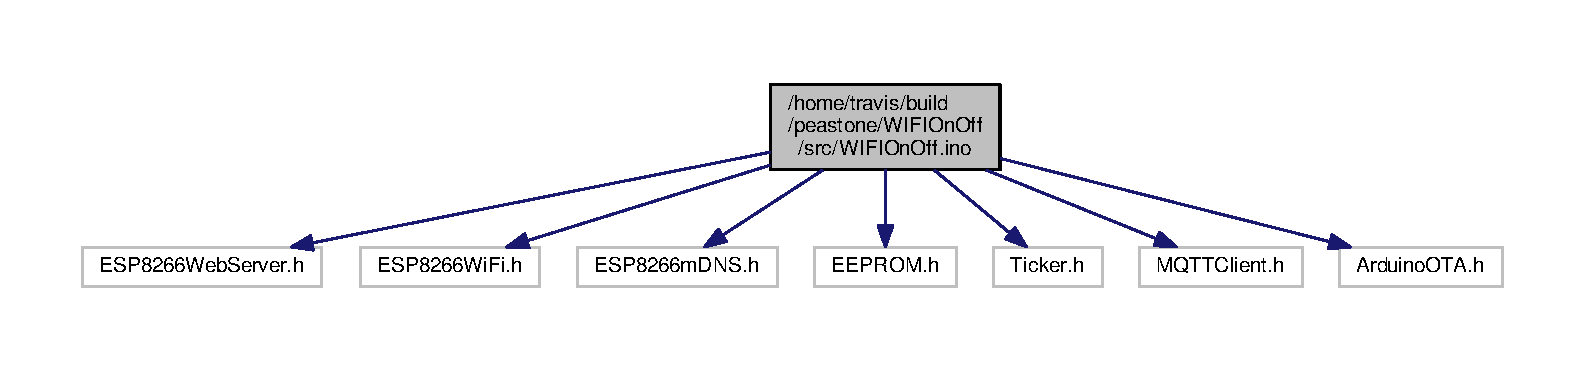
\includegraphics[width=350pt]{WIFIOnOff_8ino__incl}
\end{center}
\end{figure}
\subsection*{Macros}
\begin{DoxyCompactItemize}
\item 
\#define \hyperlink{WIFIOnOff_8ino_a111429b8fcdec5c5148837425261c18f}{S\-E\-R\-I\-A\-L\-\_\-\-P\-R\-I\-N\-T\-I\-N\-G}
\begin{DoxyCompactList}\small\item\em Define S\-E\-R\-I\-A\-L\-\_\-\-P\-R\-I\-N\-T\-I\-N\-G if you want to enable serial communication. \end{DoxyCompactList}\item 
\#define \hyperlink{WIFIOnOff_8ino_a59912dabf54ca43542cdc292e80d5742}{N\-U\-M\-E\-R\-I\-C\-\_\-\-R\-E\-S\-P\-O\-N\-S\-E}
\begin{DoxyCompactList}\small\item\em Define N\-U\-M\-E\-R\-I\-C\-\_\-\-R\-E\-S\-P\-O\-N\-S\-E if you want the \hyperlink{WIFIOnOff_8ino_a0524591f2a058a4f26f16579245db356}{mqtt\-Client} to publish \char`\"{}1\char`\"{} or \char`\"{}0\char`\"{} instead of \char`\"{}on\char`\"{} or \char`\"{}off\char`\"{}. \end{DoxyCompactList}\item 
\#define \hyperlink{WIFIOnOff_8ino_a05aa5fbe8a67eecb3e1d318cc590b4f9}{O\-U\-T\-P\-U\-T\-\_\-\-R\-E\-L\-A\-Y\-\_\-\-S\-T\-A\-T\-E\-\_\-\-O\-N\-\_\-\-G\-R\-E\-E\-N\-\_\-\-S\-T\-A\-T\-U\-S\-\_\-\-L\-E\-D}
\begin{DoxyCompactList}\small\item\em The state of the relay is visible through the blue L\-E\-D (connected == L\-E\-D shines). Define O\-U\-T\-P\-U\-T\-\_\-\-R\-E\-L\-A\-Y\-\_\-\-S\-T\-A\-T\-E\-\_\-\-O\-N\-\_\-\-G\-R\-E\-E\-N\-\_\-\-S\-T\-A\-T\-U\-S\-\_\-\-L\-E\-D, if you want the state of the relay being visible also on the green L\-E\-D (connected == L\-E\-D shines). \end{DoxyCompactList}\item 
\#define \hyperlink{WIFIOnOff_8ino_a29b6e2877e1ad309ad7f24c22f97eed1}{D\-E\-V\-\_\-\-O\-T\-A\-\_\-\-U\-P\-D\-A\-T\-E\-S}
\begin{DoxyCompactList}\small\item\em Define D\-E\-V\-\_\-\-O\-T\-A\-\_\-\-U\-P\-D\-A\-T\-E\-S if you want to perform O\-T\-A updates for development with Arduino I\-D\-E. \end{DoxyCompactList}\item 
\#define \hyperlink{WIFIOnOff_8ino_afc670eb8e8858f7ddbbecf997a99dbca}{D\-E\-V\-\_\-\-O\-T\-A\-\_\-\-P\-A\-S\-S\-W\-D}~\char`\"{}Cwpv\-Vz\-R33g\-K\-Y\char`\"{}
\begin{DoxyCompactList}\small\item\em Define the password to protect O\-T\-A with D\-E\-V\-\_\-\-O\-T\-A\-\_\-\-P\-A\-S\-S\-W\-D. This is not a high security procedure. \end{DoxyCompactList}\item 
\#define \hyperlink{WIFIOnOff_8ino_af0c74d8a61960bcc6f7e06acc3dda4c3}{T\-R\-I\-G\-G\-E\-R\-\_\-\-T\-I\-M\-E\-\_\-\-W\-P\-S}~7000
\begin{DoxyCompactList}\small\item\em time in ms to wait until W\-P\-S request is triggered when pressing the button (see \hyperlink{WIFIOnOff_8ino_acd4d58af93c899ee9a03131727b1cf34}{press\-Handler()}) \end{DoxyCompactList}\item 
\#define \hyperlink{WIFIOnOff_8ino_a65378513c8fda212e6ad80723ebfa2b7}{T\-R\-I\-G\-G\-E\-R\-\_\-\-T\-I\-M\-E\-\_\-\-W\-I\-F\-I\-\_\-\-D\-A\-T\-A\-\_\-\-R\-E\-S\-E\-T}~30000
\begin{DoxyCompactList}\small\item\em time in ms to wait until the W\-I\-F\-I configuration reset \end{DoxyCompactList}\item 
\#define \hyperlink{WIFIOnOff_8ino_a1d71187e9e78d5bd8e38f8bd84edcfbd}{T\-R\-I\-G\-G\-E\-R\-\_\-\-T\-I\-M\-E\-\_\-\-F\-A\-C\-T\-O\-R\-Y\-\_\-\-R\-E\-S\-E\-T}~60000
\begin{DoxyCompactList}\small\item\em time in ms to wait until factory reset is triggered when pressing the button (see \hyperlink{WIFIOnOff_8ino_acd4d58af93c899ee9a03131727b1cf34}{press\-Handler()}) \end{DoxyCompactList}\item 
\#define \hyperlink{WIFIOnOff_8ino_a0906dae4a42c1fef9ec0cd0a5212ed4a}{H\-T\-T\-P\-\_\-\-P\-O\-R\-T}~80
\begin{DoxyCompactList}\small\item\em standard port used for the H\-T\-T\-P protocol \end{DoxyCompactList}\item 
\#define \hyperlink{WIFIOnOff_8ino_aa8632baff6bbb5004385998918f1e6bd}{M\-Q\-T\-T\-\_\-\-P\-O\-R\-T}~1883
\begin{DoxyCompactList}\small\item\em standard port used for the M\-Q\-T\-T protocol \end{DoxyCompactList}\item 
\#define \hyperlink{WIFIOnOff_8ino_a87a8a26f2f6a9e14484ae0efabe91c99}{T\-I\-M\-E\-\_\-\-H\-A\-L\-F\-\_\-\-A\-\_\-\-S\-E\-C\-O\-N\-D}~500
\begin{DoxyCompactList}\small\item\em definition of the timespan of half a second \end{DoxyCompactList}\item 
\#define \hyperlink{WIFIOnOff_8ino_af01b3f2fe9f05e4ead3b1957d5402397}{T\-I\-M\-E\-\_\-\-Q\-U\-A\-R\-T\-E\-R\-\_\-\-S\-E\-C\-O\-N\-D}~250
\begin{DoxyCompactList}\small\item\em definition of the timespan of a quarter of a second \end{DoxyCompactList}\item 
\#define \hyperlink{WIFIOnOff_8ino_ad32448a40ca9e5dc0a62149d0f08bd5f}{T\-I\-M\-E\-\_\-\-E\-E\-P\-R\-O\-M\-\_\-\-W\-A\-R\-N\-I\-N\-G}~7000
\begin{DoxyCompactList}\small\item\em definition of the time the L\-E\-D stays on in case of an E\-E\-P\-R\-O\-M warning (C\-R\-C failure, initialization, E\-E\-P\-R\-O\-M incompatible) \end{DoxyCompactList}\item 
\#define \hyperlink{WIFIOnOff_8ino_a5b5893eb38e4fe69dc2acd2f974fa5cb}{C\-T\-R\-\_\-\-M\-A\-X\-\_\-\-T\-R\-I\-E\-S\-\_\-\-W\-I\-F\-I\-\_\-\-C\-O\-N\-N\-E\-C\-T\-I\-O\-N}~60
\begin{DoxyCompactList}\small\item\em maximum amount of tries to connect to W\-I\-F\-I \end{DoxyCompactList}\item 
\#define \hyperlink{WIFIOnOff_8ino_af7399e3a75be0250095968af4f94757e}{E\-E\-P\-R\-O\-M\-\_\-length}~4096
\begin{DoxyCompactList}\small\item\em E\-E\-P\-R\-O\-M\-\_\-length defines the maximum amount of bytes to be stored in the E\-E\-P\-R\-O\-M. At the time of writing, the maximum amout of bytes to be stored is 4096. \end{DoxyCompactList}\item 
\#define \hyperlink{WIFIOnOff_8ino_aa3109b452678c4716d01ff98ce34a2da}{E\-E\-P\-R\-O\-M\-\_\-version\-\_\-number}~0
\begin{DoxyCompactList}\small\item\em A C\-R\-C is calculated for the E\-E\-P\-R\-O\-M values to ensure that the values are untempered. The address of the stored C\-R\-C is at the beginning of the E\-E\-P\-R\-O\-M. \end{DoxyCompactList}\item 
\#define \hyperlink{WIFIOnOff_8ino_a573ec4699f45eaca686a077e5881d66b}{E\-E\-P\-R\-O\-M\-\_\-version\-\_\-number\-\_\-address}~0
\begin{DoxyCompactList}\small\item\em This version number is stored in E\-E\-P\-R\-O\-M. It must not be longer than one byte. The version number defined here and that one stored in E\-E\-P\-R\-O\-M are compared against each other. In case the two numbers are not equal, the E\-E\-P\-R\-O\-M is re-\//initialized. This number must change, if you change the E\-E\-P\-R\-O\-M layout, basically if you change adresses. \end{DoxyCompactList}\item 
\#define \hyperlink{WIFIOnOff_8ino_ab384daae78d017828d89c6d9c697021a}{E\-E\-P\-R\-O\-M\-\_\-address\-\_\-\-C\-R\-C}~1
\begin{DoxyCompactList}\small\item\em The E\-E\-P\-R\-O\-M version number is stored at this address. \end{DoxyCompactList}\item 
\#define \hyperlink{WIFIOnOff_8ino_af12bb22226c8f91f856f93ef2ddad3ec}{E\-E\-P\-R\-O\-M\-\_\-size\-\_\-\-C\-R\-C}~(sizeof(unsigned long))
\begin{DoxyCompactList}\small\item\em A C\-R\-C is calculated for the E\-E\-P\-R\-O\-M values to ensure that the values are untempered. The size of the stored C\-R\-C is defined by this macro. \end{DoxyCompactList}\item 
\#define \hyperlink{WIFIOnOff_8ino_a4e45a9ad8583fe2db7f42052e0a7ac95}{E\-E\-P\-R\-O\-M\-\_\-address\-\_\-start}~(\hyperlink{WIFIOnOff_8ino_ab384daae78d017828d89c6d9c697021a}{E\-E\-P\-R\-O\-M\-\_\-address\-\_\-\-C\-R\-C} + \hyperlink{WIFIOnOff_8ino_af12bb22226c8f91f856f93ef2ddad3ec}{E\-E\-P\-R\-O\-M\-\_\-size\-\_\-\-C\-R\-C})
\begin{DoxyCompactList}\small\item\em A C\-R\-C is calculated for the E\-E\-P\-R\-O\-M values to ensure that the values are untempered. The C\-R\-C takes some space to be stored in the E\-E\-P\-R\-O\-M. The start address takes this into account. \end{DoxyCompactList}\item 
\#define \hyperlink{WIFIOnOff_8ino_a06c93cd8175c0a438c20922e313645bd}{E\-E\-P\-R\-O\-M\-\_\-enabled}~0x\-E\-B
\begin{DoxyCompactList}\small\item\em If this magic number is set, a defined functionality is enabled. \end{DoxyCompactList}\item 
\#define \hyperlink{WIFIOnOff_8ino_a11fbf1b754b9209b6bdd4ebcb0c3e677}{E\-E\-P\-R\-O\-M\-\_\-enabled\-\_\-size}~1
\begin{DoxyCompactList}\small\item\em The amount of storage needed by \hyperlink{WIFIOnOff_8ino_a06c93cd8175c0a438c20922e313645bd}{E\-E\-P\-R\-O\-M\-\_\-enabled} in E\-E\-P\-R\-O\-M. \end{DoxyCompactList}\item 
\#define \hyperlink{WIFIOnOff_8ino_a6912b1d0bb01613405a6827632e6d6f4}{E\-E\-P\-R\-O\-M\-\_\-init\-\_\-value}~0x00
\begin{DoxyCompactList}\small\item\em If an init value is set, a defined functionality is disabled. The init value is also used to initialize the E\-E\-P\-R\-O\-M in \hyperlink{WIFIOnOff_8ino_a3d5cf434e34fce7db249185369616a32}{setup\-E\-E\-P\-R\-O\-M()}. \end{DoxyCompactList}\item 
\#define \hyperlink{WIFIOnOff_8ino_ad4bdfcba39f823c70e99abea4dc16ffb}{E\-E\-P\-R\-O\-M\-\_\-address\-\_\-\-W\-P\-S\-\_\-configured}~\hyperlink{WIFIOnOff_8ino_a4e45a9ad8583fe2db7f42052e0a7ac95}{E\-E\-P\-R\-O\-M\-\_\-address\-\_\-start}
\begin{DoxyCompactList}\small\item\em W\-P\-S is the only choice to connect to W\-I\-F\-I. This shall improve usability. The state of W\-P\-S is stored in E\-E\-P\-R\-O\-M at this address. The value 0x00 was chosen as it terminates Strings, which leads to perfect default data. \end{DoxyCompactList}\item 
\#define \hyperlink{WIFIOnOff_8ino_a604b9f83bce537df8060d5bb69480c76}{E\-E\-P\-R\-O\-M\-\_\-address\-\_\-\-M\-Q\-T\-T\-\_\-server\-\_\-configured}~(\hyperlink{WIFIOnOff_8ino_ad4bdfcba39f823c70e99abea4dc16ffb}{E\-E\-P\-R\-O\-M\-\_\-address\-\_\-\-W\-P\-S\-\_\-configured} + \hyperlink{WIFIOnOff_8ino_a11fbf1b754b9209b6bdd4ebcb0c3e677}{E\-E\-P\-R\-O\-M\-\_\-enabled\-\_\-size})
\begin{DoxyCompactList}\small\item\em This flag is used to check whether \hyperlink{WIFIOnOff_8ino_a020889fcca6224d14f4d3f4241ca4467}{mqtt\-Server} has already been initialized with the value of the M\-Q\-T\-T-\/\-Server (D\-N\-S name or I\-P) \end{DoxyCompactList}\item 
\#define \hyperlink{WIFIOnOff_8ino_add6dd801239610f299da096ea9b87383}{E\-E\-P\-R\-O\-M\-\_\-address\-\_\-\-M\-Q\-T\-T\-\_\-server}~(\hyperlink{WIFIOnOff_8ino_a604b9f83bce537df8060d5bb69480c76}{E\-E\-P\-R\-O\-M\-\_\-address\-\_\-\-M\-Q\-T\-T\-\_\-server\-\_\-configured} + \hyperlink{WIFIOnOff_8ino_a11fbf1b754b9209b6bdd4ebcb0c3e677}{E\-E\-P\-R\-O\-M\-\_\-enabled\-\_\-size})
\begin{DoxyCompactList}\small\item\em The variable \hyperlink{WIFIOnOff_8ino_a020889fcca6224d14f4d3f4241ca4467}{mqtt\-Server} which contains the value of the M\-Q\-T\-T-\/\-Server (D\-N\-S name or I\-P) is restored after startup from E\-E\-P\-R\-O\-M, if M\-Q\-T\-T is configured (\hyperlink{WIFIOnOff_8ino_a604b9f83bce537df8060d5bb69480c76}{E\-E\-P\-R\-O\-M\-\_\-address\-\_\-\-M\-Q\-T\-T\-\_\-server\-\_\-configured}). The stored bytes can be found at this address. \end{DoxyCompactList}\item 
\#define \hyperlink{WIFIOnOff_8ino_ac060eafb02eba00d33cad29f38819d4a}{E\-E\-P\-R\-O\-M\-\_\-size\-\_\-\-M\-Q\-T\-T\-\_\-server}~256
\begin{DoxyCompactList}\small\item\em The maximum amount of bytes used to store the M\-Q\-T\-T server address. This address can be either an I\-P or a D\-N\-S name. D\-N\-S names are restricted to 255 octets. As a string is zero-\/terminated, one byte more is used. For more information, look at R\-F\-C 1035. \end{DoxyCompactList}\end{DoxyCompactItemize}
\subsection*{Functions}
\begin{DoxyCompactItemize}
\item 
unsigned long \hyperlink{WIFIOnOff_8ino_a16ef77fe42b6e5a700dd2445f0aaa24f}{calculate\-\_\-crc} ()
\begin{DoxyCompactList}\small\item\em This function calculates a C\-R\-C checksum for the E\-E\-P\-R\-O\-M. It is taken from\-: \href{https://www.arduino.cc/en/Tutorial/EEPROMCrc}{\tt https\-://www.\-arduino.\-cc/en/\-Tutorial/\-E\-E\-P\-R\-O\-M\-Crc}. \end{DoxyCompactList}\item 
void \hyperlink{WIFIOnOff_8ino_a1dd9db8c49797d8536247d1fba49cfe7}{store\-C\-R\-C} ()
\begin{DoxyCompactList}\small\item\em This function calculates the C\-R\-C value of the values in the E\-E\-P\-R\-O\-M with the help of function \hyperlink{WIFIOnOff_8ino_a16ef77fe42b6e5a700dd2445f0aaa24f}{calculate\-\_\-crc()}. The resulting C\-R\-C checksum is written to \hyperlink{WIFIOnOff_8ino_ab384daae78d017828d89c6d9c697021a}{E\-E\-P\-R\-O\-M\-\_\-address\-\_\-\-C\-R\-C}. The caller must still call E\-E\-P\-R\-O\-M.\-commit() afterwards to really trigger a write to E\-E\-P\-R\-O\-M. \end{DoxyCompactList}\item 
unsigned long \hyperlink{WIFIOnOff_8ino_a80ac0ebe45e95ee7e439f2aeea333124}{retrieve\-C\-R\-C} ()
\begin{DoxyCompactList}\small\item\em This function reads the C\-R\-C value stored at \hyperlink{WIFIOnOff_8ino_ab384daae78d017828d89c6d9c697021a}{E\-E\-P\-R\-O\-M\-\_\-address\-\_\-\-C\-R\-C}. \end{DoxyCompactList}\item 
bool \hyperlink{WIFIOnOff_8ino_aeeada0076ef68a04f4794f91e727ae5a}{check\-C\-R\-C} ()
\begin{DoxyCompactList}\small\item\em This function calculates the C\-R\-C value for the bytes stored in the E\-E\-P\-R\-O\-M with the help of function \hyperlink{WIFIOnOff_8ino_a16ef77fe42b6e5a700dd2445f0aaa24f}{calculate\-\_\-crc()} and compares the result to the C\-R\-C which was read from E\-E\-P\-R\-O\-M with the help of function \hyperlink{WIFIOnOff_8ino_a80ac0ebe45e95ee7e439f2aeea333124}{retrieve\-C\-R\-C()}. \end{DoxyCompactList}\item 
void \hyperlink{WIFIOnOff_8ino_a6e14ea51750122bd7a906b9dcf896c53}{store\-E\-E\-P\-R\-O\-M\-Version\-Number} ()
\begin{DoxyCompactList}\small\item\em This function stores the \hyperlink{WIFIOnOff_8ino_aa3109b452678c4716d01ff98ce34a2da}{E\-E\-P\-R\-O\-M\-\_\-version\-\_\-number} in E\-E\-P\-R\-O\-M. \end{DoxyCompactList}\item 
bool \hyperlink{WIFIOnOff_8ino_afd23421ffd3823e5dafd4205f499fd2c}{check\-E\-E\-P\-R\-O\-M\-Version\-Number} ()
\begin{DoxyCompactList}\small\item\em This function checks the \hyperlink{WIFIOnOff_8ino_aa3109b452678c4716d01ff98ce34a2da}{E\-E\-P\-R\-O\-M\-\_\-version\-\_\-number} stored in E\-E\-P\-R\-O\-M against the version number required by the latest E\-E\-P\-R\-O\-M layout. \end{DoxyCompactList}\item 
void \hyperlink{WIFIOnOff_8ino_accde2e704135909387a34453e0dc1293}{init\-E\-E\-P\-R\-O\-M} ()
\begin{DoxyCompactList}\small\item\em This function writes default data (\hyperlink{WIFIOnOff_8ino_a6912b1d0bb01613405a6827632e6d6f4}{E\-E\-P\-R\-O\-M\-\_\-init\-\_\-value}) to E\-E\-P\-R\-O\-M and stores C\-R\-C and the \hyperlink{WIFIOnOff_8ino_aa3109b452678c4716d01ff98ce34a2da}{E\-E\-P\-R\-O\-M\-\_\-version\-\_\-number}. \end{DoxyCompactList}\item 
void \hyperlink{WIFIOnOff_8ino_a3d5cf434e34fce7db249185369616a32}{setup\-E\-E\-P\-R\-O\-M} ()
\begin{DoxyCompactList}\small\item\em This function is setting up the E\-E\-P\-R\-O\-M. If the C\-R\-C check fails, the E\-E\-P\-R\-O\-M will be overwritten with init values. The C\-R\-C check makes only sense at initialization phase. Afterwards, the data is buffered by E\-E\-P\-R\-O\-M lib in R\-A\-M. \end{DoxyCompactList}\item 
void \hyperlink{WIFIOnOff_8ino_a6a76f6c6d6e85f2215f0451b12f1db54}{switch\-Off\-L\-E\-D} ()
\begin{DoxyCompactList}\small\item\em This function is used to switch the L\-E\-D off. It keeps track of the internal state \hyperlink{WIFIOnOff_8ino_aa1ef40baec048d45fac1d51afc521d40}{state\-L\-E\-D\-On}. \end{DoxyCompactList}\item 
void \hyperlink{WIFIOnOff_8ino_a46be1cdf6842e46fb3ba46a60f024aa0}{switch\-On\-L\-E\-D} ()
\begin{DoxyCompactList}\small\item\em This function is used to switch the L\-E\-D on. It keeps track of the internal state \hyperlink{WIFIOnOff_8ino_aa1ef40baec048d45fac1d51afc521d40}{state\-L\-E\-D\-On}. \end{DoxyCompactList}\item 
void \hyperlink{WIFIOnOff_8ino_aeaf97294d049f17c3eef4add9a4df1ec}{toggle\-L\-E\-D} ()
\begin{DoxyCompactList}\small\item\em This function is used to toggle the L\-E\-D. Indirectly, it keeps track of the internal state \hyperlink{WIFIOnOff_8ino_aa1ef40baec048d45fac1d51afc521d40}{state\-L\-E\-D\-On}. \end{DoxyCompactList}\item 
bool \hyperlink{WIFIOnOff_8ino_af4164c2bb2661c7427bd66ecd2f8aace}{get\-State\-L\-E\-D\-On} ()
\begin{DoxyCompactList}\small\item\em This function is used to get the state of the L\-E\-D. It returns \hyperlink{WIFIOnOff_8ino_aa1ef40baec048d45fac1d51afc521d40}{state\-L\-E\-D\-On}. \end{DoxyCompactList}\item 
void \hyperlink{WIFIOnOff_8ino_af43969e915aec75ff3f318d585e0606a}{feedback\-E\-E\-P\-R\-O\-M\-Init} ()
\begin{DoxyCompactList}\small\item\em This function is called to give the user feedback that the E\-E\-P\-R\-O\-M has been re-\//initialized. This means that all the user-\/entered data is gone and the device needs to be reconfigured. \end{DoxyCompactList}\item 
void \hyperlink{WIFIOnOff_8ino_aed631ac5d7f4338966a6a187e1057258}{feedback\-Quick\-Blink} ()
\begin{DoxyCompactList}\small\item\em This function is called to give the user feedback about the menu the user selected. It will blink fast for a short period of time. The user has the choice to release and select the menu or to wait for the next menu. By counting the \hyperlink{WIFIOnOff_8ino_aed631ac5d7f4338966a6a187e1057258}{feedback\-Quick\-Blink()}-\/events, the user can determine which menu is selected, when the button is released now. \end{DoxyCompactList}\item 
void \hyperlink{WIFIOnOff_8ino_a29d61ce203f552333381a79f4993da69}{feedback\-W\-I\-F\-Iis\-Connecting} ()
\begin{DoxyCompactList}\small\item\em This function is called to give the user feedback that W\-I\-F\-I is about to connect. It will blink at a medium rate. \end{DoxyCompactList}\item 
bool \hyperlink{WIFIOnOff_8ino_a347d10bac439b6c073df93cbf5522f28}{get\-User\-Action\-Feedback\-Request} ()
\begin{DoxyCompactList}\small\item\em Getter function for \hyperlink{WIFIOnOff_8ino_a3e5c7c27259449622535aee1125f275a}{user\-Action\-Feedback\-Request}. \end{DoxyCompactList}\item 
bool \hyperlink{WIFIOnOff_8ino_a0185fd92dbcb609528b98244ee37430c}{set\-User\-Action\-Feedback\-Request} ()
\begin{DoxyCompactList}\small\item\em Setter function for \hyperlink{WIFIOnOff_8ino_a3e5c7c27259449622535aee1125f275a}{user\-Action\-Feedback\-Request}. The user should be notified that a menu can be selected. \end{DoxyCompactList}\item 
bool \hyperlink{WIFIOnOff_8ino_a2f07f10222db3144a4a271ddcb81cdde}{unset\-User\-Action\-Feedback\-Request} ()
\begin{DoxyCompactList}\small\item\em Setter function for \hyperlink{WIFIOnOff_8ino_a3e5c7c27259449622535aee1125f275a}{user\-Action\-Feedback\-Request}. The user has been notified that a menu can be selected. \end{DoxyCompactList}\item 
bool \hyperlink{WIFIOnOff_8ino_a7ed5532c3a832fa15a2865ee80cbfdda}{check\-Wi\-Fi\-Configured} ()
\begin{DoxyCompactList}\small\item\em This function checks whether W\-P\-S has already been performed once. In this case, one can directly connect to Wi\-Fi. \end{DoxyCompactList}\item 
void \hyperlink{WIFIOnOff_8ino_a3ebcee2a9d20137810223c6813e54787}{set\-Wi\-Fi\-Configured} ()
\begin{DoxyCompactList}\small\item\em This function is a setter function which sets Wi\-Fi to configured, which means that W\-P\-S has already been performed successfully. This function is only called in \hyperlink{WIFIOnOff_8ino_aa51eb2a71952e54dba6130be21b3a1d7}{perform\-W\-P\-S()}. The configuration is saved to E\-E\-P\-R\-O\-M. \end{DoxyCompactList}\item 
void \hyperlink{WIFIOnOff_8ino_ac782bcb28cf6c4cf77d8a408fe02c2f9}{unset\-Wi\-Fi\-Configured} ()
\begin{DoxyCompactList}\small\item\em This function is a setter function which sets Wi\-Fi to not configured, which means that W\-P\-S is necessary before connecting to W\-I\-F\-I. The configuration is saved to E\-E\-P\-R\-O\-M. \end{DoxyCompactList}\item 
void \hyperlink{WIFIOnOff_8ino_aa51eb2a71952e54dba6130be21b3a1d7}{perform\-W\-P\-S} ()
\begin{DoxyCompactList}\small\item\em This function is used to trigger W\-P\-S. If W\-P\-S has been successful, \hyperlink{WIFIOnOff_8ino_a3ebcee2a9d20137810223c6813e54787}{set\-Wi\-Fi\-Configured()} is executed and \hyperlink{WIFIOnOff_8ino_a86eebd69aeee5bbb5e648fc099b4b360}{unset\-W\-P\-S\-Request()} is called. \end{DoxyCompactList}\item 
String \hyperlink{WIFIOnOff_8ino_a688bc5c57984763646a5dd2f72943255}{get\-Client\-I\-D} ()
\begin{DoxyCompactList}\small\item\em This function returns the client name used for M\-Q\-T\-T, see \hyperlink{WIFIOnOff_8ino_a9ad5cb858c24c53a6eaa846b713bd120}{mqtt\-Connect()}. \end{DoxyCompactList}\item 
bool \hyperlink{WIFIOnOff_8ino_a31eed9b3718a60b96c1fea76590a3fc5}{connect\-To\-Wi\-Fi} ()
\begin{DoxyCompactList}\small\item\em This function tries to connect to W\-I\-F\-I. \end{DoxyCompactList}\item 
void \hyperlink{WIFIOnOff_8ino_aa61ca7b9fb98de7d85d230a82ea7de28}{setup\-M\-D\-N\-S} ()
\begin{DoxyCompactList}\small\item\em This function sets up M\-D\-N\-S. \end{DoxyCompactList}\item 
bool \hyperlink{WIFIOnOff_8ino_a7e0fb4debe9d6029fd560490e0d89062}{check\-Wi\-Fi\-Connected} ()
\begin{DoxyCompactList}\small\item\em This function checks whether W\-I\-F\-I is connected. \end{DoxyCompactList}\item 
bool \hyperlink{WIFIOnOff_8ino_a3361cdf5888fc635d5ae5d83747d50d6}{get\-W\-P\-S\-Request} ()
\begin{DoxyCompactList}\small\item\em Getter function for \hyperlink{WIFIOnOff_8ino_a002d6cec57f207948ee9f62a3fbc12fe}{wps\-Requested}. \end{DoxyCompactList}\item 
void \hyperlink{WIFIOnOff_8ino_a86eebd69aeee5bbb5e648fc099b4b360}{unset\-W\-P\-S\-Request} ()
\begin{DoxyCompactList}\small\item\em Setter function to unset \hyperlink{WIFIOnOff_8ino_a002d6cec57f207948ee9f62a3fbc12fe}{wps\-Requested}. \end{DoxyCompactList}\item 
void \hyperlink{WIFIOnOff_8ino_af2a784e9ea129440dd303530ab9e97a1}{set\-W\-P\-S\-Request} ()
\begin{DoxyCompactList}\small\item\em Setter function to set \hyperlink{WIFIOnOff_8ino_a002d6cec57f207948ee9f62a3fbc12fe}{wps\-Requested}. \end{DoxyCompactList}\item 
bool \hyperlink{WIFIOnOff_8ino_aa79761488d06c15b10258afefb215020}{get\-Wifi\-Reset\-Requested} ()
\begin{DoxyCompactList}\small\item\em Getter function for \hyperlink{WIFIOnOff_8ino_a1ef1b3b96ca3b7c432a5c202037bcd43}{wifi\-Reset\-Requested}. \end{DoxyCompactList}\item 
void \hyperlink{WIFIOnOff_8ino_a359226c1dba04041902ec5451ada2aae}{set\-Wifi\-Reset\-Requested} ()
\begin{DoxyCompactList}\small\item\em Setter function to set \hyperlink{WIFIOnOff_8ino_a1ef1b3b96ca3b7c432a5c202037bcd43}{wifi\-Reset\-Requested}. \end{DoxyCompactList}\item 
void \hyperlink{WIFIOnOff_8ino_a0e963d26058822266a054c999cf33ece}{unset\-Wifi\-Reset\-Requested} ()
\begin{DoxyCompactList}\small\item\em Setter function to unsset \hyperlink{WIFIOnOff_8ino_a1ef1b3b96ca3b7c432a5c202037bcd43}{wifi\-Reset\-Requested}. \end{DoxyCompactList}\item 
void \hyperlink{WIFIOnOff_8ino_ae850a8f5a550a31d8433eddf41a11d44}{disconnect\-Relay} ()
\begin{DoxyCompactList}\small\item\em This function is used to disconnect the relay from the mains. It keeps track of the internal state \hyperlink{WIFIOnOff_8ino_a48a5ee80a30c37768bf1e198f1ee5692}{state\-Relay\-Connected}. \end{DoxyCompactList}\item 
void \hyperlink{WIFIOnOff_8ino_a6eda13f766d5d36ba8bcbe7c252c2ab8}{connect\-Relay} ()
\begin{DoxyCompactList}\small\item\em This function is used to connect the relay to the mains. It keeps track of the internal state \hyperlink{WIFIOnOff_8ino_a48a5ee80a30c37768bf1e198f1ee5692}{state\-Relay\-Connected}. \end{DoxyCompactList}\item 
bool \hyperlink{WIFIOnOff_8ino_aefabc9bd763a51753669e6c249140abc}{get\-State\-Relay\-Connected} ()
\begin{DoxyCompactList}\small\item\em This function is used to get the connection state of the relay with the mains. It returns \hyperlink{WIFIOnOff_8ino_a48a5ee80a30c37768bf1e198f1ee5692}{state\-Relay\-Connected}. \end{DoxyCompactList}\item 
void \hyperlink{WIFIOnOff_8ino_a2d92a759a6fa273c581f3fa4243fa1d9}{toggle\-Relay} ()
\begin{DoxyCompactList}\small\item\em This function is used to toggle the connection of the relay with the mains. Indirectly, it keeps track of the internal state \hyperlink{WIFIOnOff_8ino_a48a5ee80a30c37768bf1e198f1ee5692}{state\-Relay\-Connected}. \end{DoxyCompactList}\item 
void \hyperlink{WIFIOnOff_8ino_a4b7676f0d3c07948850fd833023d7783}{configure\-Outputs} ()
\begin{DoxyCompactList}\small\item\em This function configures the output pins of the microcontroller. \end{DoxyCompactList}\item 
String \hyperlink{WIFIOnOff_8ino_a1ec8a91d3b174c2cfee9eaf852f11c1e}{render\-Header} ()
\begin{DoxyCompactList}\small\item\em This function returns the first part of a H\-T\-M\-L file which is reused for all responses. \end{DoxyCompactList}\item 
String \hyperlink{WIFIOnOff_8ino_a1c9dd84a6d6ca1ea206f310605cc049d}{render\-Relay} (bool \hyperlink{WIFIOnOff_8ino_a48a5ee80a30c37768bf1e198f1ee5692}{state\-Relay\-Connected})
\begin{DoxyCompactList}\small\item\em This function returns the middle part of a H\-T\-M\-L file to. \end{DoxyCompactList}\item 
String \hyperlink{WIFIOnOff_8ino_a4dfcb1cefe2bee38d172e3f327c1a72d}{render\-M\-Q\-T\-T\-Server\-Settings} (String stored\-Server\-Name, String failure\-Msg, bool state\-M\-Q\-T\-T\-Activated, bool state\-M\-Q\-T\-T\-Connected)
\begin{DoxyCompactList}\small\item\em This function returns the middle part of a H\-T\-M\-L file to. \end{DoxyCompactList}\item 
String \hyperlink{WIFIOnOff_8ino_a12a8bd3c3a1288633c3eade6ee8e77cf}{render\-Footer} ()
\begin{DoxyCompactList}\small\item\em This function returns the last part of a H\-T\-M\-L file which is reused for all responses. \end{DoxyCompactList}\item 
void \hyperlink{WIFIOnOff_8ino_ab913592c54bd79feda56cbdc86f44641}{mqtt\-Control\-Relay} (String \&topic, String \&payload)
\begin{DoxyCompactList}\small\item\em Callback which is called when M\-Q\-T\-T receives an incoming topic. \end{DoxyCompactList}\item 
void \hyperlink{WIFIOnOff_8ino_a42318ba7ac1f636b3bd64bf83a99dee2}{restore\-M\-Q\-T\-T\-Configuration\-From\-E\-E\-P\-R\-O\-M} ()
\begin{DoxyCompactList}\small\item\em Read back M\-Q\-T\-T server / broker name from E\-E\-P\-R\-O\-M and store it in global variable \hyperlink{WIFIOnOff_8ino_a020889fcca6224d14f4d3f4241ca4467}{mqtt\-Server}. Read back whether M\-Q\-T\-T is configured and store it in global variable \hyperlink{WIFIOnOff_8ino_a3f27c574110acbefe064ca29a7ce289d}{state\-M\-Q\-T\-T\-Configured}. \end{DoxyCompactList}\item 
void \hyperlink{WIFIOnOff_8ino_a006d783b06cfbafe0c614692c894e2ec}{save\-M\-Q\-T\-T\-Configuration\-To\-E\-E\-P\-R\-O\-M} ()
\begin{DoxyCompactList}\small\item\em Store M\-Q\-T\-T server / broker name (\hyperlink{WIFIOnOff_8ino_a020889fcca6224d14f4d3f4241ca4467}{mqtt\-Server}) and state (configured or not, \hyperlink{WIFIOnOff_8ino_a3f27c574110acbefe064ca29a7ce289d}{state\-M\-Q\-T\-T\-Configured}) in E\-E\-P\-R\-O\-M. \end{DoxyCompactList}\item 
void \hyperlink{WIFIOnOff_8ino_a3a04a0e88b0687b8c017addfed120950}{configure\-M\-Q\-T\-T} ()
\begin{DoxyCompactList}\small\item\em Configure new M\-Q\-T\-T server / broker. This will. \end{DoxyCompactList}\item 
void \hyperlink{WIFIOnOff_8ino_a104eb4efa9523edca8048af6e38d235f}{set\-M\-Q\-T\-T\-Server} (String input)
\begin{DoxyCompactList}\small\item\em Setter function for M\-Q\-T\-T server / broker \hyperlink{WIFIOnOff_8ino_a020889fcca6224d14f4d3f4241ca4467}{mqtt\-Server}. \end{DoxyCompactList}\item 
String \hyperlink{WIFIOnOff_8ino_a0914c7b7faa1375475836dc6115f1077}{get\-M\-Q\-T\-T\-Server} ()
\begin{DoxyCompactList}\small\item\em Getter function for M\-Q\-T\-T server / broker \hyperlink{WIFIOnOff_8ino_a020889fcca6224d14f4d3f4241ca4467}{mqtt\-Server}. \end{DoxyCompactList}\item 
void \hyperlink{WIFIOnOff_8ino_aad359baa91c446e57ccd6d77ebf49b5d}{set\-State\-M\-Q\-T\-T\-Configured} (bool input)
\begin{DoxyCompactList}\small\item\em Setter function for \hyperlink{WIFIOnOff_8ino_a3f27c574110acbefe064ca29a7ce289d}{state\-M\-Q\-T\-T\-Configured}. \end{DoxyCompactList}\item 
bool \hyperlink{WIFIOnOff_8ino_afc46fe517d2d628cdf59870d4f09060c}{get\-State\-M\-Q\-T\-T\-Configured} ()
\begin{DoxyCompactList}\small\item\em Getter function for \hyperlink{WIFIOnOff_8ino_a3f27c574110acbefe064ca29a7ce289d}{state\-M\-Q\-T\-T\-Configured}. \end{DoxyCompactList}\item 
void \hyperlink{WIFIOnOff_8ino_a26ae153af75c3844e61d4cd39be0b9d9}{set\-M\-Q\-T\-T\-Outgoing\-Topic} (String input)
\begin{DoxyCompactList}\small\item\em Setter function for \hyperlink{WIFIOnOff_8ino_a2311f2b74fe46d3f9e8072b3694deee5}{mqtt\-Outgoing\-Topic}. \end{DoxyCompactList}\item 
String \hyperlink{WIFIOnOff_8ino_a92b654456d82f73760cda8b83c5a0ca6}{get\-M\-Q\-T\-T\-Outgoing\-Topic} ()
\begin{DoxyCompactList}\small\item\em Getter function for \hyperlink{WIFIOnOff_8ino_a2311f2b74fe46d3f9e8072b3694deee5}{mqtt\-Outgoing\-Topic}. \end{DoxyCompactList}\item 
void \hyperlink{WIFIOnOff_8ino_a4beec40a2400bae93ac3aa8e2f701d13}{set\-M\-Q\-T\-T\-Incoming\-Topic} (String input)
\begin{DoxyCompactList}\small\item\em Setter function for \hyperlink{WIFIOnOff_8ino_a686cf2365a7075bc5f72d01c99b3a9f2}{mqtt\-Incoming\-Topic}. \end{DoxyCompactList}\item 
bool \hyperlink{WIFIOnOff_8ino_af5189bf4d6c6b3d4a90bf76335456740}{check\-M\-Q\-T\-T\-Connected} ()
\begin{DoxyCompactList}\small\item\em Get M\-Q\-T\-T connection state. \end{DoxyCompactList}\item 
void \hyperlink{WIFIOnOff_8ino_a9ad5cb858c24c53a6eaa846b713bd120}{mqtt\-Connect} ()
\begin{DoxyCompactList}\small\item\em This function connects to broker and. \end{DoxyCompactList}\item 
void \hyperlink{WIFIOnOff_8ino_a92e8e72a8c9bd699aefa63b65c4bc30c}{mqtt\-Publish} ()
\begin{DoxyCompactList}\small\item\em With the call of this function, \hyperlink{WIFIOnOff_8ino_a0524591f2a058a4f26f16579245db356}{mqtt\-Client} publishes the state of the relay (\hyperlink{WIFIOnOff_8ino_aefabc9bd763a51753669e6c249140abc}{get\-State\-Relay\-Connected()}) on the outgoing topic (\hyperlink{WIFIOnOff_8ino_a92b654456d82f73760cda8b83c5a0ca6}{get\-M\-Q\-T\-T\-Outgoing\-Topic()}) to the M\-Q\-T\-T server / broker. The macro \hyperlink{WIFIOnOff_8ino_a59912dabf54ca43542cdc292e80d5742}{N\-U\-M\-E\-R\-I\-C\-\_\-\-R\-E\-S\-P\-O\-N\-S\-E} is taken into account. \end{DoxyCompactList}\item 
bool \hyperlink{WIFIOnOff_8ino_a3523db85b2f83ce089a2a733d7a025ad}{is\-Not\-Whitelisted} (char c)
\begin{DoxyCompactList}\small\item\em This function is used for filtering out X\-S\-S attacks. This is done by whitelisting. \end{DoxyCompactList}\item 
bool \hyperlink{WIFIOnOff_8ino_a3251df1e6168789bae584b4063d5a59d}{mqtt\-Server\-Valid} (String \hyperlink{WIFIOnOff_8ino_a020889fcca6224d14f4d3f4241ca4467}{mqtt\-Server})
\begin{DoxyCompactList}\small\item\em This function is used to check whether mqtt\-Server is valid. Therefore, it is checked that the. \end{DoxyCompactList}\item 
void \hyperlink{WIFIOnOff_8ino_a50409543b7c4c4fb48e60ec35fbda3f3}{configure\-Web\-Server} ()
\begin{DoxyCompactList}\small\item\em This function is used configure the webserver. The webserver is configured by defining callback functions for handling incoming requests on. \end{DoxyCompactList}\item 
void \hyperlink{WIFIOnOff_8ino_afec1c2962185272a8c87843f95d205ad}{perform\-Factory\-Reset} ()
\begin{DoxyCompactList}\small\item\em Perform factory reset. \end{DoxyCompactList}\item 
bool \hyperlink{WIFIOnOff_8ino_a3e9603214a47595af27b6e16f635734d}{get\-Factory\-Reset\-Requested} ()
\begin{DoxyCompactList}\small\item\em Getter function for \hyperlink{WIFIOnOff_8ino_a4768e99cded5c5493ba789b0555c80fc}{factory\-Reset\-Requested}. \end{DoxyCompactList}\item 
void \hyperlink{WIFIOnOff_8ino_a974b42331b531d9c0ec0d5be4d745078}{set\-Factory\-Reset\-Requested} ()
\begin{DoxyCompactList}\small\item\em Setter function to set \hyperlink{WIFIOnOff_8ino_a4768e99cded5c5493ba789b0555c80fc}{factory\-Reset\-Requested}. \end{DoxyCompactList}\item 
void \hyperlink{WIFIOnOff_8ino_a1da84f44cf0a8afe3ad725de0cae4c19}{unset\-Factory\-Reset\-Requested} ()
\begin{DoxyCompactList}\small\item\em Setter function to unset \hyperlink{WIFIOnOff_8ino_a4768e99cded5c5493ba789b0555c80fc}{factory\-Reset\-Requested}. \end{DoxyCompactList}\item 
void \hyperlink{WIFIOnOff_8ino_acd4d58af93c899ee9a03131727b1cf34}{press\-Handler} ()
\begin{DoxyCompactList}\small\item\em This function triggers. \end{DoxyCompactList}\item 
void \hyperlink{WIFIOnOff_8ino_a7dfd9b79bc5a37d7df40207afbc5431f}{setup} (void)
\begin{DoxyCompactList}\small\item\em This function is executed once at the startup of the microcontroller. \end{DoxyCompactList}\item 
void \hyperlink{WIFIOnOff_8ino_a0b33edabd7f1c4e4a0bf32c67269be2f}{loop} (void)
\begin{DoxyCompactList}\small\item\em This function is executed in a loop after \hyperlink{WIFIOnOff_8ino_a7dfd9b79bc5a37d7df40207afbc5431f}{setup(void)} has been called. \end{DoxyCompactList}\end{DoxyCompactItemize}
\subsection*{Variables}
\begin{DoxyCompactItemize}
\item 
String \hyperlink{WIFIOnOff_8ino_ac4144c663334d0f32b58e62981300160}{R\-E\-P\-O\-S\-I\-T\-O\-R\-Y\-\_\-\-U\-R\-L\-\_\-\-S\-T\-R\-I\-N\-G} = \char`\"{}https\-://github.\-com/peastone/W\-I\-F\-I\-On\-Off\char`\"{}
\begin{DoxyCompactList}\small\item\em Contains a link to the code repository which is embedded in the rendered H\-T\-M\-L files in the function \hyperlink{WIFIOnOff_8ino_a12a8bd3c3a1288633c3eade6ee8e77cf}{render\-Footer()}. \end{DoxyCompactList}\item 
const int \hyperlink{WIFIOnOff_8ino_aea49499f7c0ed08f20649e96024455ab}{pin\-L\-E\-D} = 13
\begin{DoxyCompactList}\small\item\em Constant to map the green L\-E\-D of the Sonoff S20. \end{DoxyCompactList}\item 
bool \hyperlink{WIFIOnOff_8ino_aa1ef40baec048d45fac1d51afc521d40}{state\-L\-E\-D\-On} = false
\begin{DoxyCompactList}\small\item\em State to track whether the L\-E\-D is on. \end{DoxyCompactList}\item 
bool \hyperlink{WIFIOnOff_8ino_a3e5c7c27259449622535aee1125f275a}{user\-Action\-Feedback\-Request} = false
\begin{DoxyCompactList}\small\item\em State to track whether the user should be notified that a menu can be selected by releasing the button. \end{DoxyCompactList}\item 
Wi\-Fi\-Client \hyperlink{WIFIOnOff_8ino_a64f7c60366b0a82c42d7a1dbf4e9505a}{wifi\-Client}
\begin{DoxyCompactList}\small\item\em Necessary to initialize a M\-Q\-T\-T\-Client object. \end{DoxyCompactList}\item 
bool \hyperlink{WIFIOnOff_8ino_a002d6cec57f207948ee9f62a3fbc12fe}{wps\-Requested} = false
\begin{DoxyCompactList}\small\item\em State to track whether the W\-P\-S has been requested. \end{DoxyCompactList}\item 
bool \hyperlink{WIFIOnOff_8ino_a1ef1b3b96ca3b7c432a5c202037bcd43}{wifi\-Reset\-Requested} = false
\begin{DoxyCompactList}\small\item\em State to track whether the deletion of W\-I\-F\-I data has been requested. \end{DoxyCompactList}\item 
bool \hyperlink{WIFIOnOff_8ino_a48a5ee80a30c37768bf1e198f1ee5692}{state\-Relay\-Connected} = false
\begin{DoxyCompactList}\small\item\em State to track whether the L\-E\-D is connected to the mains. \end{DoxyCompactList}\item 
const int \hyperlink{WIFIOnOff_8ino_aa4021c86d826785a0f0bcac11a38d30e}{pin\-Relay} = 12
\begin{DoxyCompactList}\small\item\em Constant to map the relay of the Sonoff S20. \end{DoxyCompactList}\item 
M\-Q\-T\-T\-Client \hyperlink{WIFIOnOff_8ino_a0524591f2a058a4f26f16579245db356}{mqtt\-Client}
\begin{DoxyCompactList}\small\item\em central object to manage M\-Q\-T\-T \end{DoxyCompactList}\item 
String \hyperlink{WIFIOnOff_8ino_a020889fcca6224d14f4d3f4241ca4467}{mqtt\-Server} = \char`\"{}\char`\"{}
\begin{DoxyCompactList}\small\item\em Global variable to store the D\-N\-S name or I\-P address of the M\-Q\-T\-T broker. \end{DoxyCompactList}\item 
bool \hyperlink{WIFIOnOff_8ino_a3f27c574110acbefe064ca29a7ce289d}{state\-M\-Q\-T\-T\-Configured} = false
\begin{DoxyCompactList}\small\item\em State to track whether M\-Q\-T\-T is configured. \end{DoxyCompactList}\item 
String \hyperlink{WIFIOnOff_8ino_a2311f2b74fe46d3f9e8072b3694deee5}{mqtt\-Outgoing\-Topic}
\begin{DoxyCompactList}\small\item\em The topic \hyperlink{WIFIOnOff_8ino_a0524591f2a058a4f26f16579245db356}{mqtt\-Client} publishes. \end{DoxyCompactList}\item 
String \hyperlink{WIFIOnOff_8ino_a686cf2365a7075bc5f72d01c99b3a9f2}{mqtt\-Incoming\-Topic}
\begin{DoxyCompactList}\small\item\em The topic which \hyperlink{WIFIOnOff_8ino_a0524591f2a058a4f26f16579245db356}{mqtt\-Client} subscribes. \end{DoxyCompactList}\item 
E\-S\-P8266\-Web\-Server \hyperlink{WIFIOnOff_8ino_a0c2e905cdd4621947a7d6c966383e28c}{webserver}
\begin{DoxyCompactList}\small\item\em This is the webserver object. It is used to serve the user interface over H\-T\-T\-P. Per default, port 80 is used. \end{DoxyCompactList}\item 
bool \hyperlink{WIFIOnOff_8ino_a4768e99cded5c5493ba789b0555c80fc}{factory\-Reset\-Requested} = false
\begin{DoxyCompactList}\small\item\em State to track whether a factory reset has been requested. \end{DoxyCompactList}\item 
const int \hyperlink{WIFIOnOff_8ino_a4ddb8b6ae564eb22f7c74f2683a63b8e}{button\-Pin} = 0
\begin{DoxyCompactList}\small\item\em Constant to map the hardware button of the Sonoff S20. \end{DoxyCompactList}\item 
bool \hyperlink{WIFIOnOff_8ino_a80700674ee3f9a7b6ae86b0756679902}{button\-Last\-Pressed} = false
\begin{DoxyCompactList}\small\item\em State to track whether the button was pressed since \hyperlink{WIFIOnOff_8ino_acd4d58af93c899ee9a03131727b1cf34}{press\-Handler()} was called the last time. \end{DoxyCompactList}\item 
unsigned long \hyperlink{WIFIOnOff_8ino_a244ed52f592c09418e6feee15f1cecd5}{time\-Sincebutton\-Pressed} = 0
\begin{DoxyCompactList}\small\item\em State to track the time since the button was pressed. \end{DoxyCompactList}\item 
unsigned long \hyperlink{WIFIOnOff_8ino_a969fb5df6fd687b0434058fa78c25f27}{selection\-State} = 0
\begin{DoxyCompactList}\small\item\em State to track which menu the user selects, if the button is released. \end{DoxyCompactList}\item 
Ticker \hyperlink{WIFIOnOff_8ino_a4bb2542b2738619fdf76b685b10e315d}{ticker}
\begin{DoxyCompactList}\small\item\em This object is used to trigger the function press frequently. The button handler is implemented there. \end{DoxyCompactList}\end{DoxyCompactItemize}


\subsection{Detailed Description}
W\-I\-F\-I\-On\-O\-F\-F is an alternative software for the Sonoff S20 which provides a web user interface (H\-T\-T\-P) and an internet of things interface (M\-Q\-T\-T). The device can still be controlled by the normal user button. The connection to Wi\-Fi will be established by W\-P\-S for reasons of a better user experience. This device can be used in the local network without any dependency of a cloud.

Copyright (C) 2018 Siegfried Schöfer

This program is free software\-: you can redistribute it and/or modify it under the terms of the G\-N\-U General Public License as published by the Free Software Foundation, either version 3 of the License, or (at your option) any later version.

This program is distributed in the hope that it will be useful, but W\-I\-T\-H\-O\-U\-T A\-N\-Y W\-A\-R\-R\-A\-N\-T\-Y; without even the implied warranty of M\-E\-R\-C\-H\-A\-N\-T\-A\-B\-I\-L\-I\-T\-Y or F\-I\-T\-N\-E\-S\-S F\-O\-R A P\-A\-R\-T\-I\-C\-U\-L\-A\-R P\-U\-R\-P\-O\-S\-E. See the G\-N\-U General Public License for more details.

You should have received a copy of the G\-N\-U General Public License along with this program. If not, see \href{http://www.gnu.org/licenses/}{\tt http\-://www.\-gnu.\-org/licenses/}.

\begin{DoxySeeAlso}{See Also}
\href{http://mqtt.org/}{\tt http\-://mqtt.\-org/} 

\href{http://docs.oasis-open.org/mqtt/mqtt/v3.1.1/os/mqtt-v3.1.1-os.pdf}{\tt http\-://docs.\-oasis-\/open.\-org/mqtt/mqtt/v3.\-1.\-1/os/mqtt-\/v3.\-1.\-1-\/os.\-pdf} 

\href{https://github.com/esp8266/Arduino}{\tt https\-://github.\-com/esp8266/\-Arduino} 

\href{https://arduino-esp8266.readthedocs.io/en/latest/}{\tt https\-://arduino-\/esp8266.\-readthedocs.\-io/en/latest/} 

\href{https://media.readthedocs.org/pdf/arduino-esp8266/latest/arduino-esp8266.pdf}{\tt https\-://media.\-readthedocs.\-org/pdf/arduino-\/esp8266/latest/arduino-\/esp8266.\-pdf} 

\href{https://github.com/espressif/ESP8266_NONOS_SDK}{\tt https\-://github.\-com/espressif/\-E\-S\-P8266\-\_\-\-N\-O\-N\-O\-S\-\_\-\-S\-D\-K} 
\end{DoxySeeAlso}


\subsection{Macro Definition Documentation}
\hypertarget{WIFIOnOff_8ino_a5b5893eb38e4fe69dc2acd2f974fa5cb}{\index{W\-I\-F\-I\-On\-Off.\-ino@{W\-I\-F\-I\-On\-Off.\-ino}!C\-T\-R\-\_\-\-M\-A\-X\-\_\-\-T\-R\-I\-E\-S\-\_\-\-W\-I\-F\-I\-\_\-\-C\-O\-N\-N\-E\-C\-T\-I\-O\-N@{C\-T\-R\-\_\-\-M\-A\-X\-\_\-\-T\-R\-I\-E\-S\-\_\-\-W\-I\-F\-I\-\_\-\-C\-O\-N\-N\-E\-C\-T\-I\-O\-N}}
\index{C\-T\-R\-\_\-\-M\-A\-X\-\_\-\-T\-R\-I\-E\-S\-\_\-\-W\-I\-F\-I\-\_\-\-C\-O\-N\-N\-E\-C\-T\-I\-O\-N@{C\-T\-R\-\_\-\-M\-A\-X\-\_\-\-T\-R\-I\-E\-S\-\_\-\-W\-I\-F\-I\-\_\-\-C\-O\-N\-N\-E\-C\-T\-I\-O\-N}!WIFIOnOff.ino@{W\-I\-F\-I\-On\-Off.\-ino}}
\subsubsection[{C\-T\-R\-\_\-\-M\-A\-X\-\_\-\-T\-R\-I\-E\-S\-\_\-\-W\-I\-F\-I\-\_\-\-C\-O\-N\-N\-E\-C\-T\-I\-O\-N}]{\setlength{\rightskip}{0pt plus 5cm}\#define C\-T\-R\-\_\-\-M\-A\-X\-\_\-\-T\-R\-I\-E\-S\-\_\-\-W\-I\-F\-I\-\_\-\-C\-O\-N\-N\-E\-C\-T\-I\-O\-N~60}}\label{WIFIOnOff_8ino_a5b5893eb38e4fe69dc2acd2f974fa5cb}


maximum amount of tries to connect to W\-I\-F\-I 

\hypertarget{WIFIOnOff_8ino_afc670eb8e8858f7ddbbecf997a99dbca}{\index{W\-I\-F\-I\-On\-Off.\-ino@{W\-I\-F\-I\-On\-Off.\-ino}!D\-E\-V\-\_\-\-O\-T\-A\-\_\-\-P\-A\-S\-S\-W\-D@{D\-E\-V\-\_\-\-O\-T\-A\-\_\-\-P\-A\-S\-S\-W\-D}}
\index{D\-E\-V\-\_\-\-O\-T\-A\-\_\-\-P\-A\-S\-S\-W\-D@{D\-E\-V\-\_\-\-O\-T\-A\-\_\-\-P\-A\-S\-S\-W\-D}!WIFIOnOff.ino@{W\-I\-F\-I\-On\-Off.\-ino}}
\subsubsection[{D\-E\-V\-\_\-\-O\-T\-A\-\_\-\-P\-A\-S\-S\-W\-D}]{\setlength{\rightskip}{0pt plus 5cm}\#define D\-E\-V\-\_\-\-O\-T\-A\-\_\-\-P\-A\-S\-S\-W\-D~\char`\"{}Cwpv\-Vz\-R33g\-K\-Y\char`\"{}}}\label{WIFIOnOff_8ino_afc670eb8e8858f7ddbbecf997a99dbca}


Define the password to protect O\-T\-A with D\-E\-V\-\_\-\-O\-T\-A\-\_\-\-P\-A\-S\-S\-W\-D. This is not a high security procedure. 

\begin{DoxyRefDesc}{Todo}
\item[\hyperlink{todo__todo000001}{Todo}]Despite the fact that over-\/the-\/air (O\-T\-A) updates are not highly secure, it is highly recommended to change the password. This is just a very bad default. \begin{DoxySeeAlso}{See Also}
\href{https://media.readthedocs.org/pdf/arduino-esp8266/latest/arduino-esp8266.pdf}{\tt https\-://media.\-readthedocs.\-org/pdf/arduino-\/esp8266/latest/arduino-\/esp8266.\-pdf} 
\end{DoxySeeAlso}
\end{DoxyRefDesc}
\hypertarget{WIFIOnOff_8ino_a29b6e2877e1ad309ad7f24c22f97eed1}{\index{W\-I\-F\-I\-On\-Off.\-ino@{W\-I\-F\-I\-On\-Off.\-ino}!D\-E\-V\-\_\-\-O\-T\-A\-\_\-\-U\-P\-D\-A\-T\-E\-S@{D\-E\-V\-\_\-\-O\-T\-A\-\_\-\-U\-P\-D\-A\-T\-E\-S}}
\index{D\-E\-V\-\_\-\-O\-T\-A\-\_\-\-U\-P\-D\-A\-T\-E\-S@{D\-E\-V\-\_\-\-O\-T\-A\-\_\-\-U\-P\-D\-A\-T\-E\-S}!WIFIOnOff.ino@{W\-I\-F\-I\-On\-Off.\-ino}}
\subsubsection[{D\-E\-V\-\_\-\-O\-T\-A\-\_\-\-U\-P\-D\-A\-T\-E\-S}]{\setlength{\rightskip}{0pt plus 5cm}\#define D\-E\-V\-\_\-\-O\-T\-A\-\_\-\-U\-P\-D\-A\-T\-E\-S}}\label{WIFIOnOff_8ino_a29b6e2877e1ad309ad7f24c22f97eed1}


Define D\-E\-V\-\_\-\-O\-T\-A\-\_\-\-U\-P\-D\-A\-T\-E\-S if you want to perform O\-T\-A updates for development with Arduino I\-D\-E. 

\hypertarget{WIFIOnOff_8ino_ab384daae78d017828d89c6d9c697021a}{\index{W\-I\-F\-I\-On\-Off.\-ino@{W\-I\-F\-I\-On\-Off.\-ino}!E\-E\-P\-R\-O\-M\-\_\-address\-\_\-\-C\-R\-C@{E\-E\-P\-R\-O\-M\-\_\-address\-\_\-\-C\-R\-C}}
\index{E\-E\-P\-R\-O\-M\-\_\-address\-\_\-\-C\-R\-C@{E\-E\-P\-R\-O\-M\-\_\-address\-\_\-\-C\-R\-C}!WIFIOnOff.ino@{W\-I\-F\-I\-On\-Off.\-ino}}
\subsubsection[{E\-E\-P\-R\-O\-M\-\_\-address\-\_\-\-C\-R\-C}]{\setlength{\rightskip}{0pt plus 5cm}\#define E\-E\-P\-R\-O\-M\-\_\-address\-\_\-\-C\-R\-C~1}}\label{WIFIOnOff_8ino_ab384daae78d017828d89c6d9c697021a}


The E\-E\-P\-R\-O\-M version number is stored at this address. 

\hypertarget{WIFIOnOff_8ino_add6dd801239610f299da096ea9b87383}{\index{W\-I\-F\-I\-On\-Off.\-ino@{W\-I\-F\-I\-On\-Off.\-ino}!E\-E\-P\-R\-O\-M\-\_\-address\-\_\-\-M\-Q\-T\-T\-\_\-server@{E\-E\-P\-R\-O\-M\-\_\-address\-\_\-\-M\-Q\-T\-T\-\_\-server}}
\index{E\-E\-P\-R\-O\-M\-\_\-address\-\_\-\-M\-Q\-T\-T\-\_\-server@{E\-E\-P\-R\-O\-M\-\_\-address\-\_\-\-M\-Q\-T\-T\-\_\-server}!WIFIOnOff.ino@{W\-I\-F\-I\-On\-Off.\-ino}}
\subsubsection[{E\-E\-P\-R\-O\-M\-\_\-address\-\_\-\-M\-Q\-T\-T\-\_\-server}]{\setlength{\rightskip}{0pt plus 5cm}\#define E\-E\-P\-R\-O\-M\-\_\-address\-\_\-\-M\-Q\-T\-T\-\_\-server~({\bf E\-E\-P\-R\-O\-M\-\_\-address\-\_\-\-M\-Q\-T\-T\-\_\-server\-\_\-configured} + {\bf E\-E\-P\-R\-O\-M\-\_\-enabled\-\_\-size})}}\label{WIFIOnOff_8ino_add6dd801239610f299da096ea9b87383}


The variable \hyperlink{WIFIOnOff_8ino_a020889fcca6224d14f4d3f4241ca4467}{mqtt\-Server} which contains the value of the M\-Q\-T\-T-\/\-Server (D\-N\-S name or I\-P) is restored after startup from E\-E\-P\-R\-O\-M, if M\-Q\-T\-T is configured (\hyperlink{WIFIOnOff_8ino_a604b9f83bce537df8060d5bb69480c76}{E\-E\-P\-R\-O\-M\-\_\-address\-\_\-\-M\-Q\-T\-T\-\_\-server\-\_\-configured}). The stored bytes can be found at this address. 

\hypertarget{WIFIOnOff_8ino_a604b9f83bce537df8060d5bb69480c76}{\index{W\-I\-F\-I\-On\-Off.\-ino@{W\-I\-F\-I\-On\-Off.\-ino}!E\-E\-P\-R\-O\-M\-\_\-address\-\_\-\-M\-Q\-T\-T\-\_\-server\-\_\-configured@{E\-E\-P\-R\-O\-M\-\_\-address\-\_\-\-M\-Q\-T\-T\-\_\-server\-\_\-configured}}
\index{E\-E\-P\-R\-O\-M\-\_\-address\-\_\-\-M\-Q\-T\-T\-\_\-server\-\_\-configured@{E\-E\-P\-R\-O\-M\-\_\-address\-\_\-\-M\-Q\-T\-T\-\_\-server\-\_\-configured}!WIFIOnOff.ino@{W\-I\-F\-I\-On\-Off.\-ino}}
\subsubsection[{E\-E\-P\-R\-O\-M\-\_\-address\-\_\-\-M\-Q\-T\-T\-\_\-server\-\_\-configured}]{\setlength{\rightskip}{0pt plus 5cm}\#define E\-E\-P\-R\-O\-M\-\_\-address\-\_\-\-M\-Q\-T\-T\-\_\-server\-\_\-configured~({\bf E\-E\-P\-R\-O\-M\-\_\-address\-\_\-\-W\-P\-S\-\_\-configured} + {\bf E\-E\-P\-R\-O\-M\-\_\-enabled\-\_\-size})}}\label{WIFIOnOff_8ino_a604b9f83bce537df8060d5bb69480c76}


This flag is used to check whether \hyperlink{WIFIOnOff_8ino_a020889fcca6224d14f4d3f4241ca4467}{mqtt\-Server} has already been initialized with the value of the M\-Q\-T\-T-\/\-Server (D\-N\-S name or I\-P) 

\hypertarget{WIFIOnOff_8ino_a4e45a9ad8583fe2db7f42052e0a7ac95}{\index{W\-I\-F\-I\-On\-Off.\-ino@{W\-I\-F\-I\-On\-Off.\-ino}!E\-E\-P\-R\-O\-M\-\_\-address\-\_\-start@{E\-E\-P\-R\-O\-M\-\_\-address\-\_\-start}}
\index{E\-E\-P\-R\-O\-M\-\_\-address\-\_\-start@{E\-E\-P\-R\-O\-M\-\_\-address\-\_\-start}!WIFIOnOff.ino@{W\-I\-F\-I\-On\-Off.\-ino}}
\subsubsection[{E\-E\-P\-R\-O\-M\-\_\-address\-\_\-start}]{\setlength{\rightskip}{0pt plus 5cm}\#define E\-E\-P\-R\-O\-M\-\_\-address\-\_\-start~({\bf E\-E\-P\-R\-O\-M\-\_\-address\-\_\-\-C\-R\-C} + {\bf E\-E\-P\-R\-O\-M\-\_\-size\-\_\-\-C\-R\-C})}}\label{WIFIOnOff_8ino_a4e45a9ad8583fe2db7f42052e0a7ac95}


A C\-R\-C is calculated for the E\-E\-P\-R\-O\-M values to ensure that the values are untempered. The C\-R\-C takes some space to be stored in the E\-E\-P\-R\-O\-M. The start address takes this into account. 

\hypertarget{WIFIOnOff_8ino_ad4bdfcba39f823c70e99abea4dc16ffb}{\index{W\-I\-F\-I\-On\-Off.\-ino@{W\-I\-F\-I\-On\-Off.\-ino}!E\-E\-P\-R\-O\-M\-\_\-address\-\_\-\-W\-P\-S\-\_\-configured@{E\-E\-P\-R\-O\-M\-\_\-address\-\_\-\-W\-P\-S\-\_\-configured}}
\index{E\-E\-P\-R\-O\-M\-\_\-address\-\_\-\-W\-P\-S\-\_\-configured@{E\-E\-P\-R\-O\-M\-\_\-address\-\_\-\-W\-P\-S\-\_\-configured}!WIFIOnOff.ino@{W\-I\-F\-I\-On\-Off.\-ino}}
\subsubsection[{E\-E\-P\-R\-O\-M\-\_\-address\-\_\-\-W\-P\-S\-\_\-configured}]{\setlength{\rightskip}{0pt plus 5cm}\#define E\-E\-P\-R\-O\-M\-\_\-address\-\_\-\-W\-P\-S\-\_\-configured~{\bf E\-E\-P\-R\-O\-M\-\_\-address\-\_\-start}}}\label{WIFIOnOff_8ino_ad4bdfcba39f823c70e99abea4dc16ffb}


W\-P\-S is the only choice to connect to W\-I\-F\-I. This shall improve usability. The state of W\-P\-S is stored in E\-E\-P\-R\-O\-M at this address. The value 0x00 was chosen as it terminates Strings, which leads to perfect default data. 

\hypertarget{WIFIOnOff_8ino_a06c93cd8175c0a438c20922e313645bd}{\index{W\-I\-F\-I\-On\-Off.\-ino@{W\-I\-F\-I\-On\-Off.\-ino}!E\-E\-P\-R\-O\-M\-\_\-enabled@{E\-E\-P\-R\-O\-M\-\_\-enabled}}
\index{E\-E\-P\-R\-O\-M\-\_\-enabled@{E\-E\-P\-R\-O\-M\-\_\-enabled}!WIFIOnOff.ino@{W\-I\-F\-I\-On\-Off.\-ino}}
\subsubsection[{E\-E\-P\-R\-O\-M\-\_\-enabled}]{\setlength{\rightskip}{0pt plus 5cm}\#define E\-E\-P\-R\-O\-M\-\_\-enabled~0x\-E\-B}}\label{WIFIOnOff_8ino_a06c93cd8175c0a438c20922e313645bd}


If this magic number is set, a defined functionality is enabled. 

\hypertarget{WIFIOnOff_8ino_a11fbf1b754b9209b6bdd4ebcb0c3e677}{\index{W\-I\-F\-I\-On\-Off.\-ino@{W\-I\-F\-I\-On\-Off.\-ino}!E\-E\-P\-R\-O\-M\-\_\-enabled\-\_\-size@{E\-E\-P\-R\-O\-M\-\_\-enabled\-\_\-size}}
\index{E\-E\-P\-R\-O\-M\-\_\-enabled\-\_\-size@{E\-E\-P\-R\-O\-M\-\_\-enabled\-\_\-size}!WIFIOnOff.ino@{W\-I\-F\-I\-On\-Off.\-ino}}
\subsubsection[{E\-E\-P\-R\-O\-M\-\_\-enabled\-\_\-size}]{\setlength{\rightskip}{0pt plus 5cm}\#define E\-E\-P\-R\-O\-M\-\_\-enabled\-\_\-size~1}}\label{WIFIOnOff_8ino_a11fbf1b754b9209b6bdd4ebcb0c3e677}


The amount of storage needed by \hyperlink{WIFIOnOff_8ino_a06c93cd8175c0a438c20922e313645bd}{E\-E\-P\-R\-O\-M\-\_\-enabled} in E\-E\-P\-R\-O\-M. 

\hypertarget{WIFIOnOff_8ino_a6912b1d0bb01613405a6827632e6d6f4}{\index{W\-I\-F\-I\-On\-Off.\-ino@{W\-I\-F\-I\-On\-Off.\-ino}!E\-E\-P\-R\-O\-M\-\_\-init\-\_\-value@{E\-E\-P\-R\-O\-M\-\_\-init\-\_\-value}}
\index{E\-E\-P\-R\-O\-M\-\_\-init\-\_\-value@{E\-E\-P\-R\-O\-M\-\_\-init\-\_\-value}!WIFIOnOff.ino@{W\-I\-F\-I\-On\-Off.\-ino}}
\subsubsection[{E\-E\-P\-R\-O\-M\-\_\-init\-\_\-value}]{\setlength{\rightskip}{0pt plus 5cm}\#define E\-E\-P\-R\-O\-M\-\_\-init\-\_\-value~0x00}}\label{WIFIOnOff_8ino_a6912b1d0bb01613405a6827632e6d6f4}


If an init value is set, a defined functionality is disabled. The init value is also used to initialize the E\-E\-P\-R\-O\-M in \hyperlink{WIFIOnOff_8ino_a3d5cf434e34fce7db249185369616a32}{setup\-E\-E\-P\-R\-O\-M()}. 

\hypertarget{WIFIOnOff_8ino_af7399e3a75be0250095968af4f94757e}{\index{W\-I\-F\-I\-On\-Off.\-ino@{W\-I\-F\-I\-On\-Off.\-ino}!E\-E\-P\-R\-O\-M\-\_\-length@{E\-E\-P\-R\-O\-M\-\_\-length}}
\index{E\-E\-P\-R\-O\-M\-\_\-length@{E\-E\-P\-R\-O\-M\-\_\-length}!WIFIOnOff.ino@{W\-I\-F\-I\-On\-Off.\-ino}}
\subsubsection[{E\-E\-P\-R\-O\-M\-\_\-length}]{\setlength{\rightskip}{0pt plus 5cm}\#define E\-E\-P\-R\-O\-M\-\_\-length~4096}}\label{WIFIOnOff_8ino_af7399e3a75be0250095968af4f94757e}


E\-E\-P\-R\-O\-M\-\_\-length defines the maximum amount of bytes to be stored in the E\-E\-P\-R\-O\-M. At the time of writing, the maximum amout of bytes to be stored is 4096. 

\begin{DoxySeeAlso}{See Also}
\href{https://git.io/vxYHO}{\tt https\-://git.\-io/vx\-Y\-H\-O} 

\href{https://git.io/vxYHG}{\tt https\-://git.\-io/vx\-Y\-H\-G} 
\end{DoxySeeAlso}
\hypertarget{WIFIOnOff_8ino_af12bb22226c8f91f856f93ef2ddad3ec}{\index{W\-I\-F\-I\-On\-Off.\-ino@{W\-I\-F\-I\-On\-Off.\-ino}!E\-E\-P\-R\-O\-M\-\_\-size\-\_\-\-C\-R\-C@{E\-E\-P\-R\-O\-M\-\_\-size\-\_\-\-C\-R\-C}}
\index{E\-E\-P\-R\-O\-M\-\_\-size\-\_\-\-C\-R\-C@{E\-E\-P\-R\-O\-M\-\_\-size\-\_\-\-C\-R\-C}!WIFIOnOff.ino@{W\-I\-F\-I\-On\-Off.\-ino}}
\subsubsection[{E\-E\-P\-R\-O\-M\-\_\-size\-\_\-\-C\-R\-C}]{\setlength{\rightskip}{0pt plus 5cm}\#define E\-E\-P\-R\-O\-M\-\_\-size\-\_\-\-C\-R\-C~(sizeof(unsigned long))}}\label{WIFIOnOff_8ino_af12bb22226c8f91f856f93ef2ddad3ec}


A C\-R\-C is calculated for the E\-E\-P\-R\-O\-M values to ensure that the values are untempered. The size of the stored C\-R\-C is defined by this macro. 

\hypertarget{WIFIOnOff_8ino_ac060eafb02eba00d33cad29f38819d4a}{\index{W\-I\-F\-I\-On\-Off.\-ino@{W\-I\-F\-I\-On\-Off.\-ino}!E\-E\-P\-R\-O\-M\-\_\-size\-\_\-\-M\-Q\-T\-T\-\_\-server@{E\-E\-P\-R\-O\-M\-\_\-size\-\_\-\-M\-Q\-T\-T\-\_\-server}}
\index{E\-E\-P\-R\-O\-M\-\_\-size\-\_\-\-M\-Q\-T\-T\-\_\-server@{E\-E\-P\-R\-O\-M\-\_\-size\-\_\-\-M\-Q\-T\-T\-\_\-server}!WIFIOnOff.ino@{W\-I\-F\-I\-On\-Off.\-ino}}
\subsubsection[{E\-E\-P\-R\-O\-M\-\_\-size\-\_\-\-M\-Q\-T\-T\-\_\-server}]{\setlength{\rightskip}{0pt plus 5cm}\#define E\-E\-P\-R\-O\-M\-\_\-size\-\_\-\-M\-Q\-T\-T\-\_\-server~256}}\label{WIFIOnOff_8ino_ac060eafb02eba00d33cad29f38819d4a}


The maximum amount of bytes used to store the M\-Q\-T\-T server address. This address can be either an I\-P or a D\-N\-S name. D\-N\-S names are restricted to 255 octets. As a string is zero-\/terminated, one byte more is used. For more information, look at R\-F\-C 1035. 

\begin{DoxySeeAlso}{See Also}
\href{https://www.ietf.org/rfc/rfc1035.txt}{\tt https\-://www.\-ietf.\-org/rfc/rfc1035.\-txt} 
\end{DoxySeeAlso}
\hypertarget{WIFIOnOff_8ino_aa3109b452678c4716d01ff98ce34a2da}{\index{W\-I\-F\-I\-On\-Off.\-ino@{W\-I\-F\-I\-On\-Off.\-ino}!E\-E\-P\-R\-O\-M\-\_\-version\-\_\-number@{E\-E\-P\-R\-O\-M\-\_\-version\-\_\-number}}
\index{E\-E\-P\-R\-O\-M\-\_\-version\-\_\-number@{E\-E\-P\-R\-O\-M\-\_\-version\-\_\-number}!WIFIOnOff.ino@{W\-I\-F\-I\-On\-Off.\-ino}}
\subsubsection[{E\-E\-P\-R\-O\-M\-\_\-version\-\_\-number}]{\setlength{\rightskip}{0pt plus 5cm}\#define E\-E\-P\-R\-O\-M\-\_\-version\-\_\-number~0}}\label{WIFIOnOff_8ino_aa3109b452678c4716d01ff98ce34a2da}


A C\-R\-C is calculated for the E\-E\-P\-R\-O\-M values to ensure that the values are untempered. The address of the stored C\-R\-C is at the beginning of the E\-E\-P\-R\-O\-M. 

\hypertarget{WIFIOnOff_8ino_a573ec4699f45eaca686a077e5881d66b}{\index{W\-I\-F\-I\-On\-Off.\-ino@{W\-I\-F\-I\-On\-Off.\-ino}!E\-E\-P\-R\-O\-M\-\_\-version\-\_\-number\-\_\-address@{E\-E\-P\-R\-O\-M\-\_\-version\-\_\-number\-\_\-address}}
\index{E\-E\-P\-R\-O\-M\-\_\-version\-\_\-number\-\_\-address@{E\-E\-P\-R\-O\-M\-\_\-version\-\_\-number\-\_\-address}!WIFIOnOff.ino@{W\-I\-F\-I\-On\-Off.\-ino}}
\subsubsection[{E\-E\-P\-R\-O\-M\-\_\-version\-\_\-number\-\_\-address}]{\setlength{\rightskip}{0pt plus 5cm}\#define E\-E\-P\-R\-O\-M\-\_\-version\-\_\-number\-\_\-address~0}}\label{WIFIOnOff_8ino_a573ec4699f45eaca686a077e5881d66b}


This version number is stored in E\-E\-P\-R\-O\-M. It must not be longer than one byte. The version number defined here and that one stored in E\-E\-P\-R\-O\-M are compared against each other. In case the two numbers are not equal, the E\-E\-P\-R\-O\-M is re-\//initialized. This number must change, if you change the E\-E\-P\-R\-O\-M layout, basically if you change adresses. 

\hypertarget{WIFIOnOff_8ino_a0906dae4a42c1fef9ec0cd0a5212ed4a}{\index{W\-I\-F\-I\-On\-Off.\-ino@{W\-I\-F\-I\-On\-Off.\-ino}!H\-T\-T\-P\-\_\-\-P\-O\-R\-T@{H\-T\-T\-P\-\_\-\-P\-O\-R\-T}}
\index{H\-T\-T\-P\-\_\-\-P\-O\-R\-T@{H\-T\-T\-P\-\_\-\-P\-O\-R\-T}!WIFIOnOff.ino@{W\-I\-F\-I\-On\-Off.\-ino}}
\subsubsection[{H\-T\-T\-P\-\_\-\-P\-O\-R\-T}]{\setlength{\rightskip}{0pt plus 5cm}\#define H\-T\-T\-P\-\_\-\-P\-O\-R\-T~80}}\label{WIFIOnOff_8ino_a0906dae4a42c1fef9ec0cd0a5212ed4a}


standard port used for the H\-T\-T\-P protocol 

\hypertarget{WIFIOnOff_8ino_aa8632baff6bbb5004385998918f1e6bd}{\index{W\-I\-F\-I\-On\-Off.\-ino@{W\-I\-F\-I\-On\-Off.\-ino}!M\-Q\-T\-T\-\_\-\-P\-O\-R\-T@{M\-Q\-T\-T\-\_\-\-P\-O\-R\-T}}
\index{M\-Q\-T\-T\-\_\-\-P\-O\-R\-T@{M\-Q\-T\-T\-\_\-\-P\-O\-R\-T}!WIFIOnOff.ino@{W\-I\-F\-I\-On\-Off.\-ino}}
\subsubsection[{M\-Q\-T\-T\-\_\-\-P\-O\-R\-T}]{\setlength{\rightskip}{0pt plus 5cm}\#define M\-Q\-T\-T\-\_\-\-P\-O\-R\-T~1883}}\label{WIFIOnOff_8ino_aa8632baff6bbb5004385998918f1e6bd}


standard port used for the M\-Q\-T\-T protocol 

\hypertarget{WIFIOnOff_8ino_a59912dabf54ca43542cdc292e80d5742}{\index{W\-I\-F\-I\-On\-Off.\-ino@{W\-I\-F\-I\-On\-Off.\-ino}!N\-U\-M\-E\-R\-I\-C\-\_\-\-R\-E\-S\-P\-O\-N\-S\-E@{N\-U\-M\-E\-R\-I\-C\-\_\-\-R\-E\-S\-P\-O\-N\-S\-E}}
\index{N\-U\-M\-E\-R\-I\-C\-\_\-\-R\-E\-S\-P\-O\-N\-S\-E@{N\-U\-M\-E\-R\-I\-C\-\_\-\-R\-E\-S\-P\-O\-N\-S\-E}!WIFIOnOff.ino@{W\-I\-F\-I\-On\-Off.\-ino}}
\subsubsection[{N\-U\-M\-E\-R\-I\-C\-\_\-\-R\-E\-S\-P\-O\-N\-S\-E}]{\setlength{\rightskip}{0pt plus 5cm}\#define N\-U\-M\-E\-R\-I\-C\-\_\-\-R\-E\-S\-P\-O\-N\-S\-E}}\label{WIFIOnOff_8ino_a59912dabf54ca43542cdc292e80d5742}


Define N\-U\-M\-E\-R\-I\-C\-\_\-\-R\-E\-S\-P\-O\-N\-S\-E if you want the \hyperlink{WIFIOnOff_8ino_a0524591f2a058a4f26f16579245db356}{mqtt\-Client} to publish \char`\"{}1\char`\"{} or \char`\"{}0\char`\"{} instead of \char`\"{}on\char`\"{} or \char`\"{}off\char`\"{}. 

\hypertarget{WIFIOnOff_8ino_a05aa5fbe8a67eecb3e1d318cc590b4f9}{\index{W\-I\-F\-I\-On\-Off.\-ino@{W\-I\-F\-I\-On\-Off.\-ino}!O\-U\-T\-P\-U\-T\-\_\-\-R\-E\-L\-A\-Y\-\_\-\-S\-T\-A\-T\-E\-\_\-\-O\-N\-\_\-\-G\-R\-E\-E\-N\-\_\-\-S\-T\-A\-T\-U\-S\-\_\-\-L\-E\-D@{O\-U\-T\-P\-U\-T\-\_\-\-R\-E\-L\-A\-Y\-\_\-\-S\-T\-A\-T\-E\-\_\-\-O\-N\-\_\-\-G\-R\-E\-E\-N\-\_\-\-S\-T\-A\-T\-U\-S\-\_\-\-L\-E\-D}}
\index{O\-U\-T\-P\-U\-T\-\_\-\-R\-E\-L\-A\-Y\-\_\-\-S\-T\-A\-T\-E\-\_\-\-O\-N\-\_\-\-G\-R\-E\-E\-N\-\_\-\-S\-T\-A\-T\-U\-S\-\_\-\-L\-E\-D@{O\-U\-T\-P\-U\-T\-\_\-\-R\-E\-L\-A\-Y\-\_\-\-S\-T\-A\-T\-E\-\_\-\-O\-N\-\_\-\-G\-R\-E\-E\-N\-\_\-\-S\-T\-A\-T\-U\-S\-\_\-\-L\-E\-D}!WIFIOnOff.ino@{W\-I\-F\-I\-On\-Off.\-ino}}
\subsubsection[{O\-U\-T\-P\-U\-T\-\_\-\-R\-E\-L\-A\-Y\-\_\-\-S\-T\-A\-T\-E\-\_\-\-O\-N\-\_\-\-G\-R\-E\-E\-N\-\_\-\-S\-T\-A\-T\-U\-S\-\_\-\-L\-E\-D}]{\setlength{\rightskip}{0pt plus 5cm}\#define O\-U\-T\-P\-U\-T\-\_\-\-R\-E\-L\-A\-Y\-\_\-\-S\-T\-A\-T\-E\-\_\-\-O\-N\-\_\-\-G\-R\-E\-E\-N\-\_\-\-S\-T\-A\-T\-U\-S\-\_\-\-L\-E\-D}}\label{WIFIOnOff_8ino_a05aa5fbe8a67eecb3e1d318cc590b4f9}


The state of the relay is visible through the blue L\-E\-D (connected == L\-E\-D shines). Define O\-U\-T\-P\-U\-T\-\_\-\-R\-E\-L\-A\-Y\-\_\-\-S\-T\-A\-T\-E\-\_\-\-O\-N\-\_\-\-G\-R\-E\-E\-N\-\_\-\-S\-T\-A\-T\-U\-S\-\_\-\-L\-E\-D, if you want the state of the relay being visible also on the green L\-E\-D (connected == L\-E\-D shines). 

\hypertarget{WIFIOnOff_8ino_a111429b8fcdec5c5148837425261c18f}{\index{W\-I\-F\-I\-On\-Off.\-ino@{W\-I\-F\-I\-On\-Off.\-ino}!S\-E\-R\-I\-A\-L\-\_\-\-P\-R\-I\-N\-T\-I\-N\-G@{S\-E\-R\-I\-A\-L\-\_\-\-P\-R\-I\-N\-T\-I\-N\-G}}
\index{S\-E\-R\-I\-A\-L\-\_\-\-P\-R\-I\-N\-T\-I\-N\-G@{S\-E\-R\-I\-A\-L\-\_\-\-P\-R\-I\-N\-T\-I\-N\-G}!WIFIOnOff.ino@{W\-I\-F\-I\-On\-Off.\-ino}}
\subsubsection[{S\-E\-R\-I\-A\-L\-\_\-\-P\-R\-I\-N\-T\-I\-N\-G}]{\setlength{\rightskip}{0pt plus 5cm}\#define S\-E\-R\-I\-A\-L\-\_\-\-P\-R\-I\-N\-T\-I\-N\-G}}\label{WIFIOnOff_8ino_a111429b8fcdec5c5148837425261c18f}


Define S\-E\-R\-I\-A\-L\-\_\-\-P\-R\-I\-N\-T\-I\-N\-G if you want to enable serial communication. 

\hypertarget{WIFIOnOff_8ino_ad32448a40ca9e5dc0a62149d0f08bd5f}{\index{W\-I\-F\-I\-On\-Off.\-ino@{W\-I\-F\-I\-On\-Off.\-ino}!T\-I\-M\-E\-\_\-\-E\-E\-P\-R\-O\-M\-\_\-\-W\-A\-R\-N\-I\-N\-G@{T\-I\-M\-E\-\_\-\-E\-E\-P\-R\-O\-M\-\_\-\-W\-A\-R\-N\-I\-N\-G}}
\index{T\-I\-M\-E\-\_\-\-E\-E\-P\-R\-O\-M\-\_\-\-W\-A\-R\-N\-I\-N\-G@{T\-I\-M\-E\-\_\-\-E\-E\-P\-R\-O\-M\-\_\-\-W\-A\-R\-N\-I\-N\-G}!WIFIOnOff.ino@{W\-I\-F\-I\-On\-Off.\-ino}}
\subsubsection[{T\-I\-M\-E\-\_\-\-E\-E\-P\-R\-O\-M\-\_\-\-W\-A\-R\-N\-I\-N\-G}]{\setlength{\rightskip}{0pt plus 5cm}\#define T\-I\-M\-E\-\_\-\-E\-E\-P\-R\-O\-M\-\_\-\-W\-A\-R\-N\-I\-N\-G~7000}}\label{WIFIOnOff_8ino_ad32448a40ca9e5dc0a62149d0f08bd5f}


definition of the time the L\-E\-D stays on in case of an E\-E\-P\-R\-O\-M warning (C\-R\-C failure, initialization, E\-E\-P\-R\-O\-M incompatible) 

\hypertarget{WIFIOnOff_8ino_a87a8a26f2f6a9e14484ae0efabe91c99}{\index{W\-I\-F\-I\-On\-Off.\-ino@{W\-I\-F\-I\-On\-Off.\-ino}!T\-I\-M\-E\-\_\-\-H\-A\-L\-F\-\_\-\-A\-\_\-\-S\-E\-C\-O\-N\-D@{T\-I\-M\-E\-\_\-\-H\-A\-L\-F\-\_\-\-A\-\_\-\-S\-E\-C\-O\-N\-D}}
\index{T\-I\-M\-E\-\_\-\-H\-A\-L\-F\-\_\-\-A\-\_\-\-S\-E\-C\-O\-N\-D@{T\-I\-M\-E\-\_\-\-H\-A\-L\-F\-\_\-\-A\-\_\-\-S\-E\-C\-O\-N\-D}!WIFIOnOff.ino@{W\-I\-F\-I\-On\-Off.\-ino}}
\subsubsection[{T\-I\-M\-E\-\_\-\-H\-A\-L\-F\-\_\-\-A\-\_\-\-S\-E\-C\-O\-N\-D}]{\setlength{\rightskip}{0pt plus 5cm}\#define T\-I\-M\-E\-\_\-\-H\-A\-L\-F\-\_\-\-A\-\_\-\-S\-E\-C\-O\-N\-D~500}}\label{WIFIOnOff_8ino_a87a8a26f2f6a9e14484ae0efabe91c99}


definition of the timespan of half a second 

\hypertarget{WIFIOnOff_8ino_af01b3f2fe9f05e4ead3b1957d5402397}{\index{W\-I\-F\-I\-On\-Off.\-ino@{W\-I\-F\-I\-On\-Off.\-ino}!T\-I\-M\-E\-\_\-\-Q\-U\-A\-R\-T\-E\-R\-\_\-\-S\-E\-C\-O\-N\-D@{T\-I\-M\-E\-\_\-\-Q\-U\-A\-R\-T\-E\-R\-\_\-\-S\-E\-C\-O\-N\-D}}
\index{T\-I\-M\-E\-\_\-\-Q\-U\-A\-R\-T\-E\-R\-\_\-\-S\-E\-C\-O\-N\-D@{T\-I\-M\-E\-\_\-\-Q\-U\-A\-R\-T\-E\-R\-\_\-\-S\-E\-C\-O\-N\-D}!WIFIOnOff.ino@{W\-I\-F\-I\-On\-Off.\-ino}}
\subsubsection[{T\-I\-M\-E\-\_\-\-Q\-U\-A\-R\-T\-E\-R\-\_\-\-S\-E\-C\-O\-N\-D}]{\setlength{\rightskip}{0pt plus 5cm}\#define T\-I\-M\-E\-\_\-\-Q\-U\-A\-R\-T\-E\-R\-\_\-\-S\-E\-C\-O\-N\-D~250}}\label{WIFIOnOff_8ino_af01b3f2fe9f05e4ead3b1957d5402397}


definition of the timespan of a quarter of a second 

\hypertarget{WIFIOnOff_8ino_a1d71187e9e78d5bd8e38f8bd84edcfbd}{\index{W\-I\-F\-I\-On\-Off.\-ino@{W\-I\-F\-I\-On\-Off.\-ino}!T\-R\-I\-G\-G\-E\-R\-\_\-\-T\-I\-M\-E\-\_\-\-F\-A\-C\-T\-O\-R\-Y\-\_\-\-R\-E\-S\-E\-T@{T\-R\-I\-G\-G\-E\-R\-\_\-\-T\-I\-M\-E\-\_\-\-F\-A\-C\-T\-O\-R\-Y\-\_\-\-R\-E\-S\-E\-T}}
\index{T\-R\-I\-G\-G\-E\-R\-\_\-\-T\-I\-M\-E\-\_\-\-F\-A\-C\-T\-O\-R\-Y\-\_\-\-R\-E\-S\-E\-T@{T\-R\-I\-G\-G\-E\-R\-\_\-\-T\-I\-M\-E\-\_\-\-F\-A\-C\-T\-O\-R\-Y\-\_\-\-R\-E\-S\-E\-T}!WIFIOnOff.ino@{W\-I\-F\-I\-On\-Off.\-ino}}
\subsubsection[{T\-R\-I\-G\-G\-E\-R\-\_\-\-T\-I\-M\-E\-\_\-\-F\-A\-C\-T\-O\-R\-Y\-\_\-\-R\-E\-S\-E\-T}]{\setlength{\rightskip}{0pt plus 5cm}\#define T\-R\-I\-G\-G\-E\-R\-\_\-\-T\-I\-M\-E\-\_\-\-F\-A\-C\-T\-O\-R\-Y\-\_\-\-R\-E\-S\-E\-T~60000}}\label{WIFIOnOff_8ino_a1d71187e9e78d5bd8e38f8bd84edcfbd}


time in ms to wait until factory reset is triggered when pressing the button (see \hyperlink{WIFIOnOff_8ino_acd4d58af93c899ee9a03131727b1cf34}{press\-Handler()}) 

\hypertarget{WIFIOnOff_8ino_a65378513c8fda212e6ad80723ebfa2b7}{\index{W\-I\-F\-I\-On\-Off.\-ino@{W\-I\-F\-I\-On\-Off.\-ino}!T\-R\-I\-G\-G\-E\-R\-\_\-\-T\-I\-M\-E\-\_\-\-W\-I\-F\-I\-\_\-\-D\-A\-T\-A\-\_\-\-R\-E\-S\-E\-T@{T\-R\-I\-G\-G\-E\-R\-\_\-\-T\-I\-M\-E\-\_\-\-W\-I\-F\-I\-\_\-\-D\-A\-T\-A\-\_\-\-R\-E\-S\-E\-T}}
\index{T\-R\-I\-G\-G\-E\-R\-\_\-\-T\-I\-M\-E\-\_\-\-W\-I\-F\-I\-\_\-\-D\-A\-T\-A\-\_\-\-R\-E\-S\-E\-T@{T\-R\-I\-G\-G\-E\-R\-\_\-\-T\-I\-M\-E\-\_\-\-W\-I\-F\-I\-\_\-\-D\-A\-T\-A\-\_\-\-R\-E\-S\-E\-T}!WIFIOnOff.ino@{W\-I\-F\-I\-On\-Off.\-ino}}
\subsubsection[{T\-R\-I\-G\-G\-E\-R\-\_\-\-T\-I\-M\-E\-\_\-\-W\-I\-F\-I\-\_\-\-D\-A\-T\-A\-\_\-\-R\-E\-S\-E\-T}]{\setlength{\rightskip}{0pt plus 5cm}\#define T\-R\-I\-G\-G\-E\-R\-\_\-\-T\-I\-M\-E\-\_\-\-W\-I\-F\-I\-\_\-\-D\-A\-T\-A\-\_\-\-R\-E\-S\-E\-T~30000}}\label{WIFIOnOff_8ino_a65378513c8fda212e6ad80723ebfa2b7}


time in ms to wait until the W\-I\-F\-I configuration reset 

\hypertarget{WIFIOnOff_8ino_af0c74d8a61960bcc6f7e06acc3dda4c3}{\index{W\-I\-F\-I\-On\-Off.\-ino@{W\-I\-F\-I\-On\-Off.\-ino}!T\-R\-I\-G\-G\-E\-R\-\_\-\-T\-I\-M\-E\-\_\-\-W\-P\-S@{T\-R\-I\-G\-G\-E\-R\-\_\-\-T\-I\-M\-E\-\_\-\-W\-P\-S}}
\index{T\-R\-I\-G\-G\-E\-R\-\_\-\-T\-I\-M\-E\-\_\-\-W\-P\-S@{T\-R\-I\-G\-G\-E\-R\-\_\-\-T\-I\-M\-E\-\_\-\-W\-P\-S}!WIFIOnOff.ino@{W\-I\-F\-I\-On\-Off.\-ino}}
\subsubsection[{T\-R\-I\-G\-G\-E\-R\-\_\-\-T\-I\-M\-E\-\_\-\-W\-P\-S}]{\setlength{\rightskip}{0pt plus 5cm}\#define T\-R\-I\-G\-G\-E\-R\-\_\-\-T\-I\-M\-E\-\_\-\-W\-P\-S~7000}}\label{WIFIOnOff_8ino_af0c74d8a61960bcc6f7e06acc3dda4c3}


time in ms to wait until W\-P\-S request is triggered when pressing the button (see \hyperlink{WIFIOnOff_8ino_acd4d58af93c899ee9a03131727b1cf34}{press\-Handler()}) 



\subsection{Function Documentation}
\hypertarget{WIFIOnOff_8ino_a16ef77fe42b6e5a700dd2445f0aaa24f}{\index{W\-I\-F\-I\-On\-Off.\-ino@{W\-I\-F\-I\-On\-Off.\-ino}!calculate\-\_\-crc@{calculate\-\_\-crc}}
\index{calculate\-\_\-crc@{calculate\-\_\-crc}!WIFIOnOff.ino@{W\-I\-F\-I\-On\-Off.\-ino}}
\subsubsection[{calculate\-\_\-crc}]{\setlength{\rightskip}{0pt plus 5cm}unsigned long calculate\-\_\-crc (
\begin{DoxyParamCaption}
{}
\end{DoxyParamCaption}
)}}\label{WIFIOnOff_8ino_a16ef77fe42b6e5a700dd2445f0aaa24f}


This function calculates a C\-R\-C checksum for the E\-E\-P\-R\-O\-M. It is taken from\-: \href{https://www.arduino.cc/en/Tutorial/EEPROMCrc}{\tt https\-://www.\-arduino.\-cc/en/\-Tutorial/\-E\-E\-P\-R\-O\-M\-Crc}. 

\begin{DoxyReturn}{Returns}
calculated C\-R\-C 
\end{DoxyReturn}


Here is the caller graph for this function\-:
\nopagebreak
\begin{figure}[H]
\begin{center}
\leavevmode
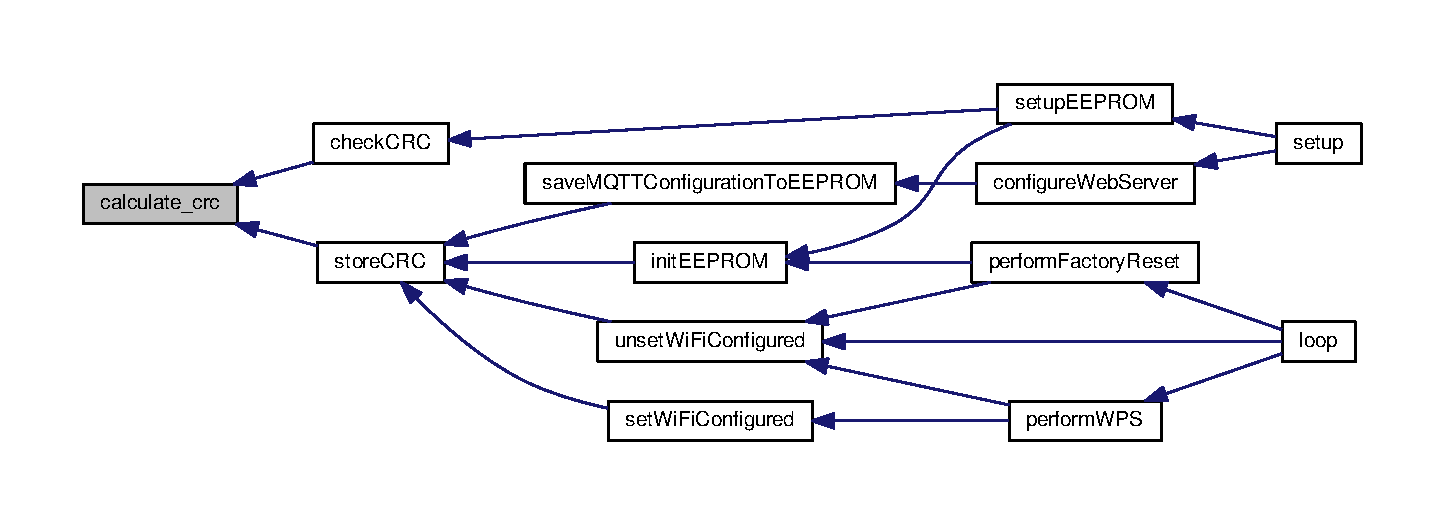
\includegraphics[width=350pt]{WIFIOnOff_8ino_a16ef77fe42b6e5a700dd2445f0aaa24f_icgraph}
\end{center}
\end{figure}


\hypertarget{WIFIOnOff_8ino_aeeada0076ef68a04f4794f91e727ae5a}{\index{W\-I\-F\-I\-On\-Off.\-ino@{W\-I\-F\-I\-On\-Off.\-ino}!check\-C\-R\-C@{check\-C\-R\-C}}
\index{check\-C\-R\-C@{check\-C\-R\-C}!WIFIOnOff.ino@{W\-I\-F\-I\-On\-Off.\-ino}}
\subsubsection[{check\-C\-R\-C}]{\setlength{\rightskip}{0pt plus 5cm}bool check\-C\-R\-C (
\begin{DoxyParamCaption}
{}
\end{DoxyParamCaption}
)}}\label{WIFIOnOff_8ino_aeeada0076ef68a04f4794f91e727ae5a}


This function calculates the C\-R\-C value for the bytes stored in the E\-E\-P\-R\-O\-M with the help of function \hyperlink{WIFIOnOff_8ino_a16ef77fe42b6e5a700dd2445f0aaa24f}{calculate\-\_\-crc()} and compares the result to the C\-R\-C which was read from E\-E\-P\-R\-O\-M with the help of function \hyperlink{WIFIOnOff_8ino_a80ac0ebe45e95ee7e439f2aeea333124}{retrieve\-C\-R\-C()}. 

\begin{DoxyReturn}{Returns}
true if calculated C\-R\-C matches stored C\-R\-C 
\end{DoxyReturn}


Here is the call graph for this function\-:
\nopagebreak
\begin{figure}[H]
\begin{center}
\leavevmode
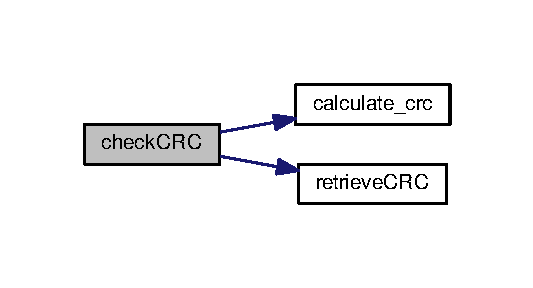
\includegraphics[width=256pt]{WIFIOnOff_8ino_aeeada0076ef68a04f4794f91e727ae5a_cgraph}
\end{center}
\end{figure}




Here is the caller graph for this function\-:
\nopagebreak
\begin{figure}[H]
\begin{center}
\leavevmode
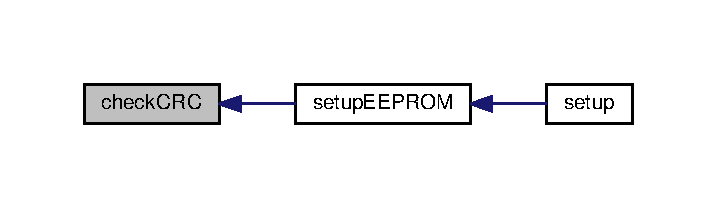
\includegraphics[width=344pt]{WIFIOnOff_8ino_aeeada0076ef68a04f4794f91e727ae5a_icgraph}
\end{center}
\end{figure}


\hypertarget{WIFIOnOff_8ino_afd23421ffd3823e5dafd4205f499fd2c}{\index{W\-I\-F\-I\-On\-Off.\-ino@{W\-I\-F\-I\-On\-Off.\-ino}!check\-E\-E\-P\-R\-O\-M\-Version\-Number@{check\-E\-E\-P\-R\-O\-M\-Version\-Number}}
\index{check\-E\-E\-P\-R\-O\-M\-Version\-Number@{check\-E\-E\-P\-R\-O\-M\-Version\-Number}!WIFIOnOff.ino@{W\-I\-F\-I\-On\-Off.\-ino}}
\subsubsection[{check\-E\-E\-P\-R\-O\-M\-Version\-Number}]{\setlength{\rightskip}{0pt plus 5cm}bool check\-E\-E\-P\-R\-O\-M\-Version\-Number (
\begin{DoxyParamCaption}
{}
\end{DoxyParamCaption}
)}}\label{WIFIOnOff_8ino_afd23421ffd3823e5dafd4205f499fd2c}


This function checks the \hyperlink{WIFIOnOff_8ino_aa3109b452678c4716d01ff98ce34a2da}{E\-E\-P\-R\-O\-M\-\_\-version\-\_\-number} stored in E\-E\-P\-R\-O\-M against the version number required by the latest E\-E\-P\-R\-O\-M layout. 

\begin{DoxyReturn}{Returns}
true, if the stored and the required E\-E\-P\-R\-O\-M version number match, false otherwise 
\end{DoxyReturn}


Here is the caller graph for this function\-:
\nopagebreak
\begin{figure}[H]
\begin{center}
\leavevmode
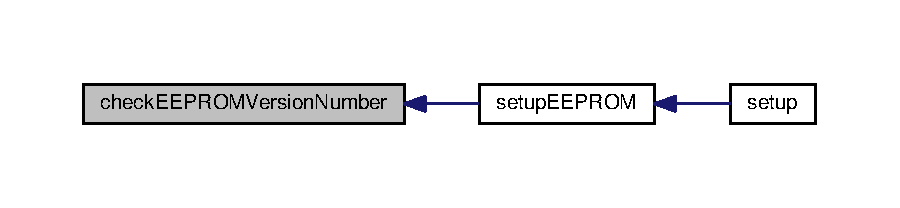
\includegraphics[width=350pt]{WIFIOnOff_8ino_afd23421ffd3823e5dafd4205f499fd2c_icgraph}
\end{center}
\end{figure}


\hypertarget{WIFIOnOff_8ino_af5189bf4d6c6b3d4a90bf76335456740}{\index{W\-I\-F\-I\-On\-Off.\-ino@{W\-I\-F\-I\-On\-Off.\-ino}!check\-M\-Q\-T\-T\-Connected@{check\-M\-Q\-T\-T\-Connected}}
\index{check\-M\-Q\-T\-T\-Connected@{check\-M\-Q\-T\-T\-Connected}!WIFIOnOff.ino@{W\-I\-F\-I\-On\-Off.\-ino}}
\subsubsection[{check\-M\-Q\-T\-T\-Connected}]{\setlength{\rightskip}{0pt plus 5cm}bool check\-M\-Q\-T\-T\-Connected (
\begin{DoxyParamCaption}
{}
\end{DoxyParamCaption}
)}}\label{WIFIOnOff_8ino_af5189bf4d6c6b3d4a90bf76335456740}


Get M\-Q\-T\-T connection state. 

\begin{DoxyReturn}{Returns}
true, if M\-Q\-T\-T is connected, false otherwise 
\end{DoxyReturn}


Here is the caller graph for this function\-:
\nopagebreak
\begin{figure}[H]
\begin{center}
\leavevmode
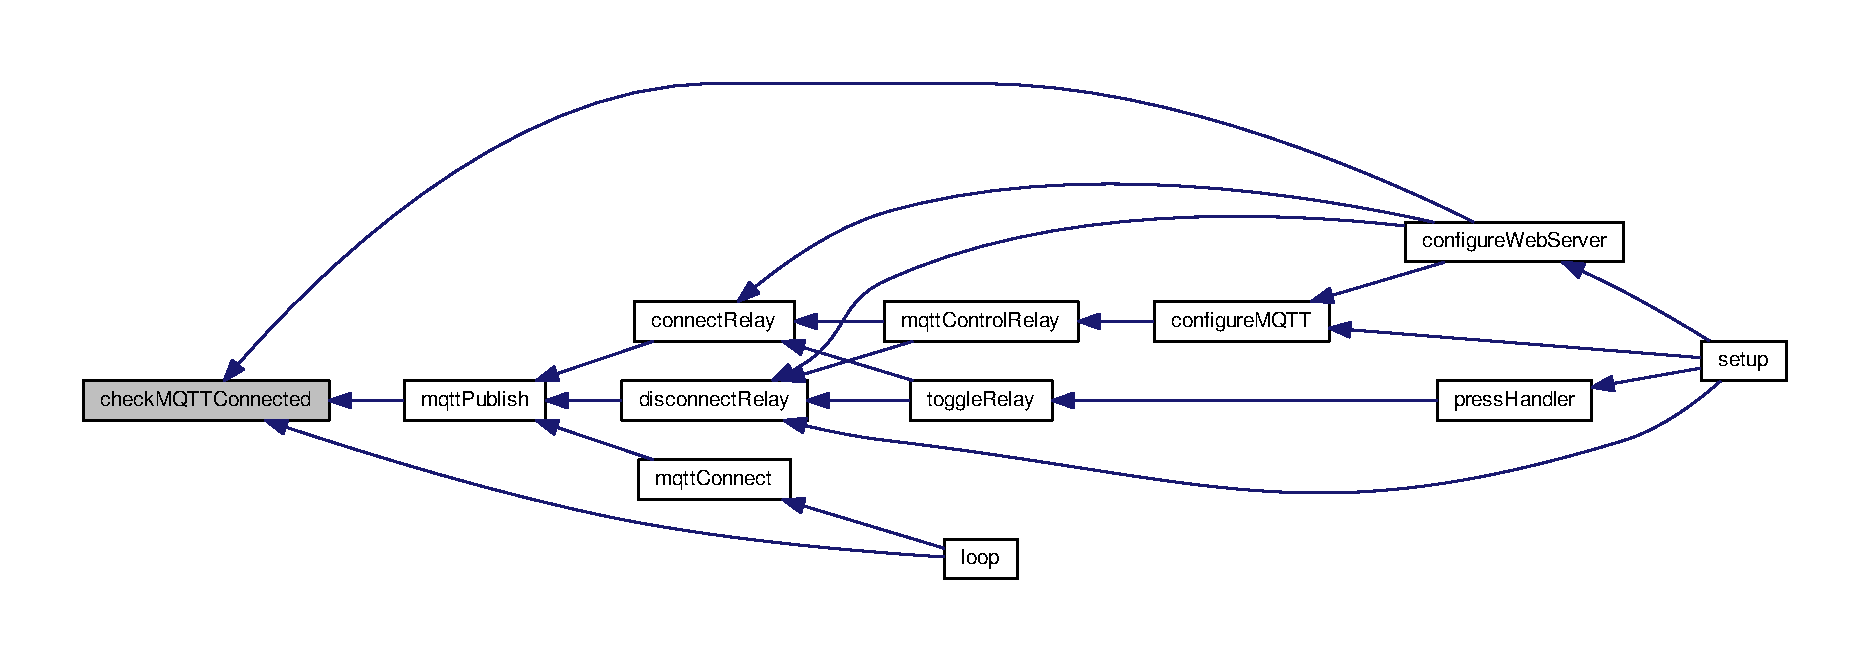
\includegraphics[width=350pt]{WIFIOnOff_8ino_af5189bf4d6c6b3d4a90bf76335456740_icgraph}
\end{center}
\end{figure}


\hypertarget{WIFIOnOff_8ino_a7ed5532c3a832fa15a2865ee80cbfdda}{\index{W\-I\-F\-I\-On\-Off.\-ino@{W\-I\-F\-I\-On\-Off.\-ino}!check\-Wi\-Fi\-Configured@{check\-Wi\-Fi\-Configured}}
\index{check\-Wi\-Fi\-Configured@{check\-Wi\-Fi\-Configured}!WIFIOnOff.ino@{W\-I\-F\-I\-On\-Off.\-ino}}
\subsubsection[{check\-Wi\-Fi\-Configured}]{\setlength{\rightskip}{0pt plus 5cm}bool check\-Wi\-Fi\-Configured (
\begin{DoxyParamCaption}
{}
\end{DoxyParamCaption}
)}}\label{WIFIOnOff_8ino_a7ed5532c3a832fa15a2865ee80cbfdda}


This function checks whether W\-P\-S has already been performed once. In this case, one can directly connect to Wi\-Fi. 

\begin{DoxyReturn}{Returns}
true if W\-P\-S has already been performed, false otherwise 
\end{DoxyReturn}


Here is the caller graph for this function\-:
\nopagebreak
\begin{figure}[H]
\begin{center}
\leavevmode
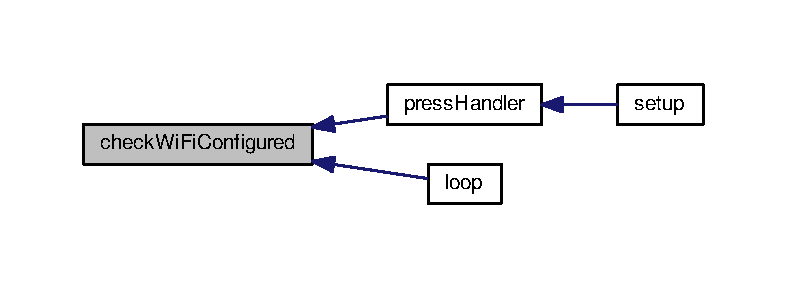
\includegraphics[width=350pt]{WIFIOnOff_8ino_a7ed5532c3a832fa15a2865ee80cbfdda_icgraph}
\end{center}
\end{figure}


\hypertarget{WIFIOnOff_8ino_a7e0fb4debe9d6029fd560490e0d89062}{\index{W\-I\-F\-I\-On\-Off.\-ino@{W\-I\-F\-I\-On\-Off.\-ino}!check\-Wi\-Fi\-Connected@{check\-Wi\-Fi\-Connected}}
\index{check\-Wi\-Fi\-Connected@{check\-Wi\-Fi\-Connected}!WIFIOnOff.ino@{W\-I\-F\-I\-On\-Off.\-ino}}
\subsubsection[{check\-Wi\-Fi\-Connected}]{\setlength{\rightskip}{0pt plus 5cm}bool check\-Wi\-Fi\-Connected (
\begin{DoxyParamCaption}
{}
\end{DoxyParamCaption}
)}}\label{WIFIOnOff_8ino_a7e0fb4debe9d6029fd560490e0d89062}


This function checks whether W\-I\-F\-I is connected. 

\begin{DoxyReturn}{Returns}
true, if Wi\-Fi is connected, false otherwise 
\end{DoxyReturn}


Here is the caller graph for this function\-:
\nopagebreak
\begin{figure}[H]
\begin{center}
\leavevmode
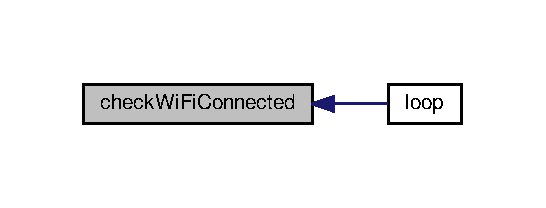
\includegraphics[width=262pt]{WIFIOnOff_8ino_a7e0fb4debe9d6029fd560490e0d89062_icgraph}
\end{center}
\end{figure}


\hypertarget{WIFIOnOff_8ino_a3a04a0e88b0687b8c017addfed120950}{\index{W\-I\-F\-I\-On\-Off.\-ino@{W\-I\-F\-I\-On\-Off.\-ino}!configure\-M\-Q\-T\-T@{configure\-M\-Q\-T\-T}}
\index{configure\-M\-Q\-T\-T@{configure\-M\-Q\-T\-T}!WIFIOnOff.ino@{W\-I\-F\-I\-On\-Off.\-ino}}
\subsubsection[{configure\-M\-Q\-T\-T}]{\setlength{\rightskip}{0pt plus 5cm}void configure\-M\-Q\-T\-T (
\begin{DoxyParamCaption}
{}
\end{DoxyParamCaption}
)}}\label{WIFIOnOff_8ino_a3a04a0e88b0687b8c017addfed120950}


Configure new M\-Q\-T\-T server / broker. This will. 


\begin{DoxyItemize}
\item disconnect the M\-Q\-T\-T client if connected
\item set the server / broker name
\item set the callback mqtt\-Conrol\-Relay() 
\end{DoxyItemize}

Here is the call graph for this function\-:
\nopagebreak
\begin{figure}[H]
\begin{center}
\leavevmode
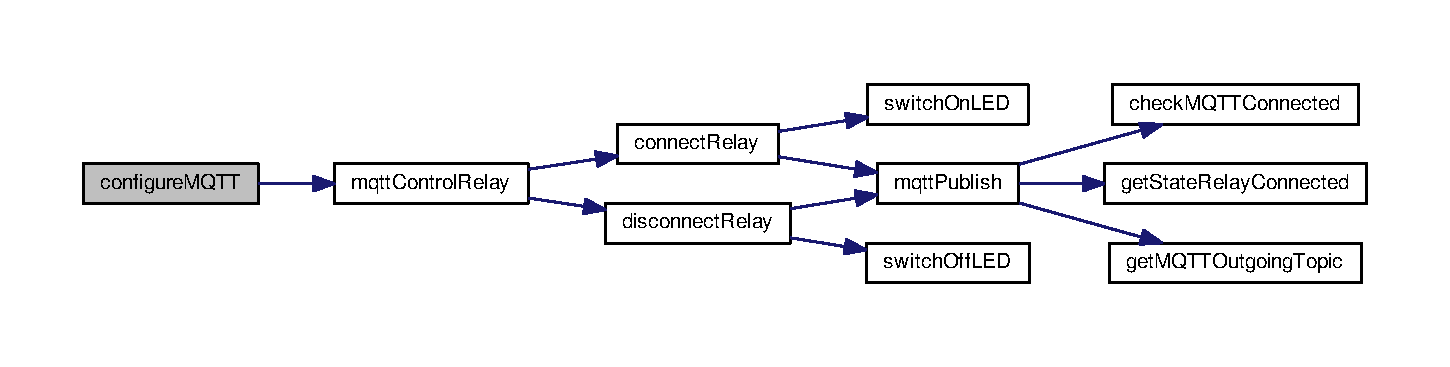
\includegraphics[width=350pt]{WIFIOnOff_8ino_a3a04a0e88b0687b8c017addfed120950_cgraph}
\end{center}
\end{figure}




Here is the caller graph for this function\-:
\nopagebreak
\begin{figure}[H]
\begin{center}
\leavevmode
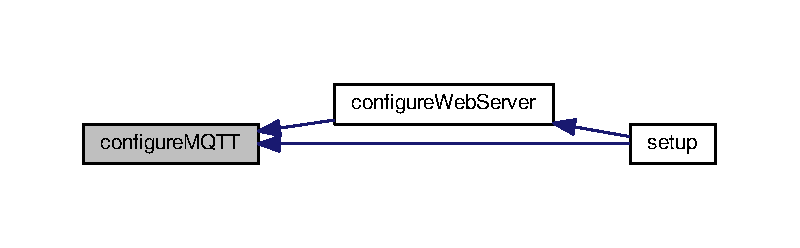
\includegraphics[width=350pt]{WIFIOnOff_8ino_a3a04a0e88b0687b8c017addfed120950_icgraph}
\end{center}
\end{figure}


\hypertarget{WIFIOnOff_8ino_a4b7676f0d3c07948850fd833023d7783}{\index{W\-I\-F\-I\-On\-Off.\-ino@{W\-I\-F\-I\-On\-Off.\-ino}!configure\-Outputs@{configure\-Outputs}}
\index{configure\-Outputs@{configure\-Outputs}!WIFIOnOff.ino@{W\-I\-F\-I\-On\-Off.\-ino}}
\subsubsection[{configure\-Outputs}]{\setlength{\rightskip}{0pt plus 5cm}void configure\-Outputs (
\begin{DoxyParamCaption}
{}
\end{DoxyParamCaption}
)}}\label{WIFIOnOff_8ino_a4b7676f0d3c07948850fd833023d7783}


This function configures the output pins of the microcontroller. 



Here is the caller graph for this function\-:
\nopagebreak
\begin{figure}[H]
\begin{center}
\leavevmode
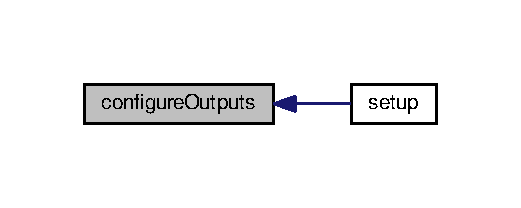
\includegraphics[width=250pt]{WIFIOnOff_8ino_a4b7676f0d3c07948850fd833023d7783_icgraph}
\end{center}
\end{figure}


\hypertarget{WIFIOnOff_8ino_a50409543b7c4c4fb48e60ec35fbda3f3}{\index{W\-I\-F\-I\-On\-Off.\-ino@{W\-I\-F\-I\-On\-Off.\-ino}!configure\-Web\-Server@{configure\-Web\-Server}}
\index{configure\-Web\-Server@{configure\-Web\-Server}!WIFIOnOff.ino@{W\-I\-F\-I\-On\-Off.\-ino}}
\subsubsection[{configure\-Web\-Server}]{\setlength{\rightskip}{0pt plus 5cm}void configure\-Web\-Server (
\begin{DoxyParamCaption}
{}
\end{DoxyParamCaption}
)}}\label{WIFIOnOff_8ino_a50409543b7c4c4fb48e60ec35fbda3f3}


This function is used configure the webserver. The webserver is configured by defining callback functions for handling incoming requests on. 


\begin{DoxyItemize}
\item /
\item /settings.html 
\end{DoxyItemize}

Here is the call graph for this function\-:
\nopagebreak
\begin{figure}[H]
\begin{center}
\leavevmode
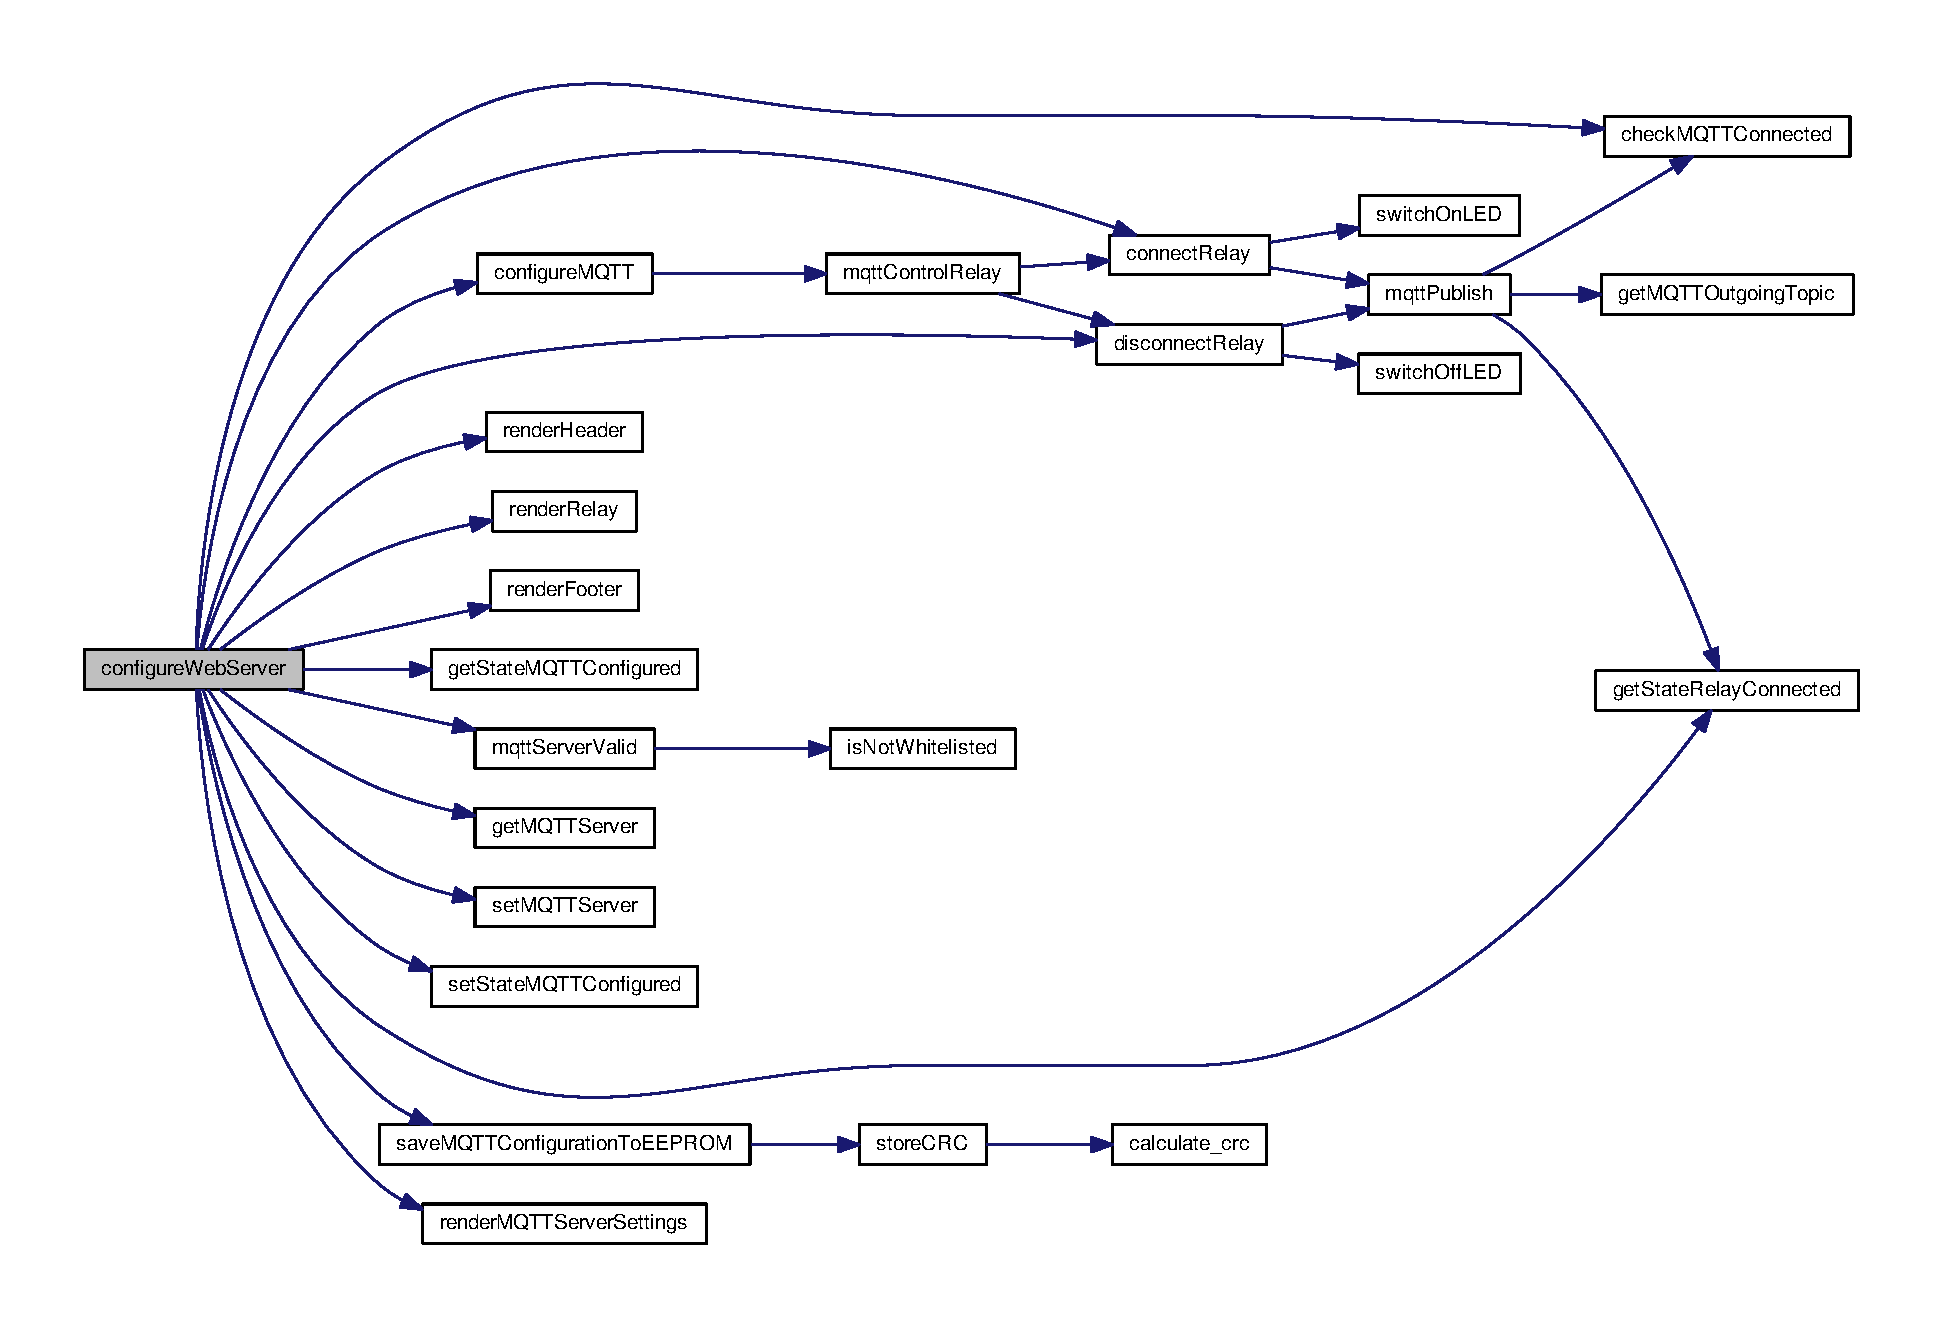
\includegraphics[width=350pt]{WIFIOnOff_8ino_a50409543b7c4c4fb48e60ec35fbda3f3_cgraph}
\end{center}
\end{figure}




Here is the caller graph for this function\-:
\nopagebreak
\begin{figure}[H]
\begin{center}
\leavevmode
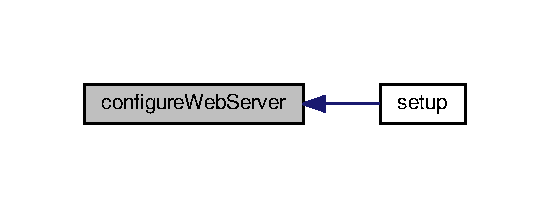
\includegraphics[width=264pt]{WIFIOnOff_8ino_a50409543b7c4c4fb48e60ec35fbda3f3_icgraph}
\end{center}
\end{figure}


\hypertarget{WIFIOnOff_8ino_a6eda13f766d5d36ba8bcbe7c252c2ab8}{\index{W\-I\-F\-I\-On\-Off.\-ino@{W\-I\-F\-I\-On\-Off.\-ino}!connect\-Relay@{connect\-Relay}}
\index{connect\-Relay@{connect\-Relay}!WIFIOnOff.ino@{W\-I\-F\-I\-On\-Off.\-ino}}
\subsubsection[{connect\-Relay}]{\setlength{\rightskip}{0pt plus 5cm}void connect\-Relay (
\begin{DoxyParamCaption}
{}
\end{DoxyParamCaption}
)}}\label{WIFIOnOff_8ino_a6eda13f766d5d36ba8bcbe7c252c2ab8}


This function is used to connect the relay to the mains. It keeps track of the internal state \hyperlink{WIFIOnOff_8ino_a48a5ee80a30c37768bf1e198f1ee5692}{state\-Relay\-Connected}. 



Here is the call graph for this function\-:
\nopagebreak
\begin{figure}[H]
\begin{center}
\leavevmode
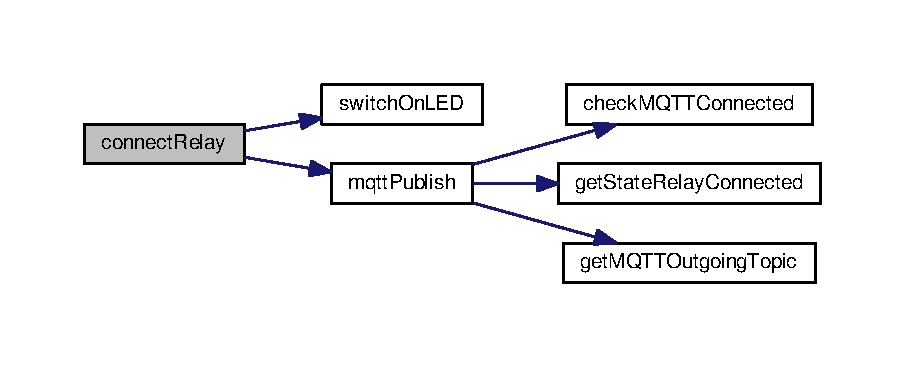
\includegraphics[width=350pt]{WIFIOnOff_8ino_a6eda13f766d5d36ba8bcbe7c252c2ab8_cgraph}
\end{center}
\end{figure}




Here is the caller graph for this function\-:
\nopagebreak
\begin{figure}[H]
\begin{center}
\leavevmode
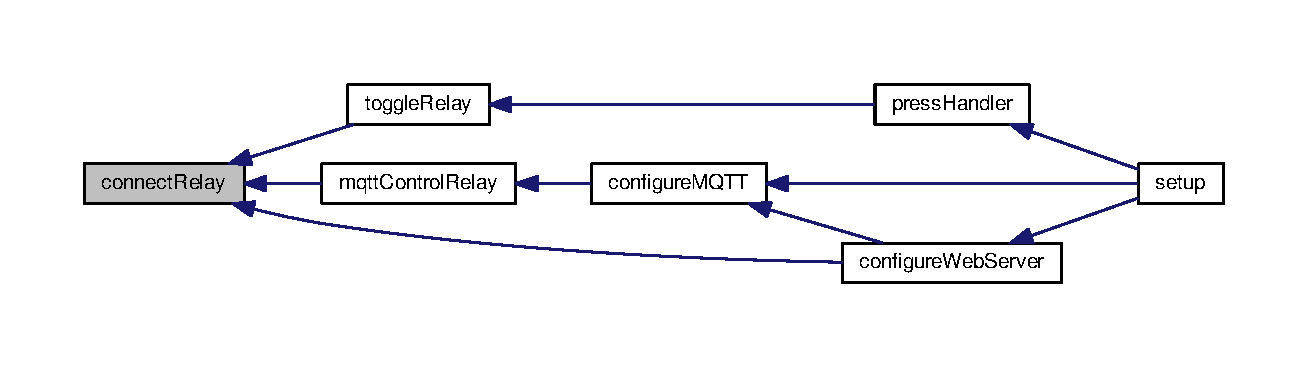
\includegraphics[width=350pt]{WIFIOnOff_8ino_a6eda13f766d5d36ba8bcbe7c252c2ab8_icgraph}
\end{center}
\end{figure}


\hypertarget{WIFIOnOff_8ino_a31eed9b3718a60b96c1fea76590a3fc5}{\index{W\-I\-F\-I\-On\-Off.\-ino@{W\-I\-F\-I\-On\-Off.\-ino}!connect\-To\-Wi\-Fi@{connect\-To\-Wi\-Fi}}
\index{connect\-To\-Wi\-Fi@{connect\-To\-Wi\-Fi}!WIFIOnOff.ino@{W\-I\-F\-I\-On\-Off.\-ino}}
\subsubsection[{connect\-To\-Wi\-Fi}]{\setlength{\rightskip}{0pt plus 5cm}bool connect\-To\-Wi\-Fi (
\begin{DoxyParamCaption}
{}
\end{DoxyParamCaption}
)}}\label{WIFIOnOff_8ino_a31eed9b3718a60b96c1fea76590a3fc5}


This function tries to connect to W\-I\-F\-I. 

\begin{DoxyReturn}{Returns}
true, if the connection was successful, false otherwise. 
\end{DoxyReturn}


Here is the call graph for this function\-:
\nopagebreak
\begin{figure}[H]
\begin{center}
\leavevmode
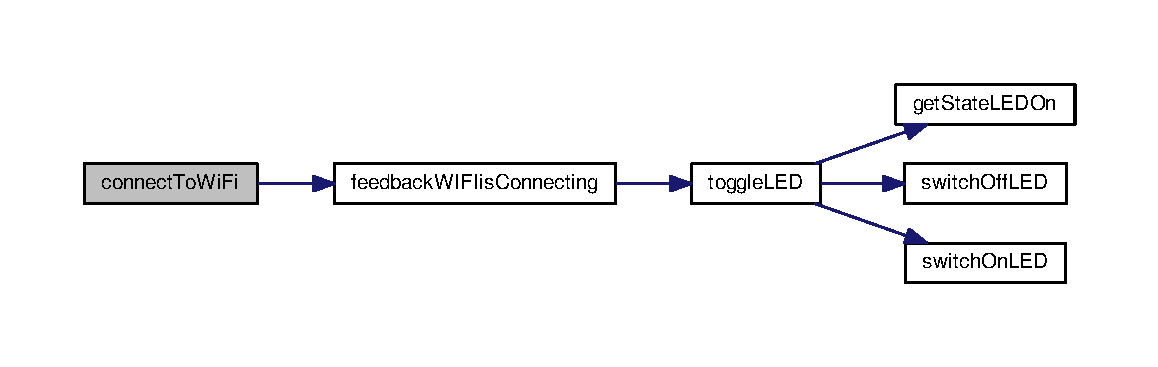
\includegraphics[width=350pt]{WIFIOnOff_8ino_a31eed9b3718a60b96c1fea76590a3fc5_cgraph}
\end{center}
\end{figure}




Here is the caller graph for this function\-:
\nopagebreak
\begin{figure}[H]
\begin{center}
\leavevmode
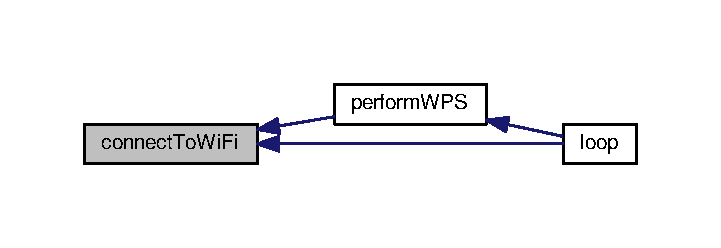
\includegraphics[width=346pt]{WIFIOnOff_8ino_a31eed9b3718a60b96c1fea76590a3fc5_icgraph}
\end{center}
\end{figure}


\hypertarget{WIFIOnOff_8ino_ae850a8f5a550a31d8433eddf41a11d44}{\index{W\-I\-F\-I\-On\-Off.\-ino@{W\-I\-F\-I\-On\-Off.\-ino}!disconnect\-Relay@{disconnect\-Relay}}
\index{disconnect\-Relay@{disconnect\-Relay}!WIFIOnOff.ino@{W\-I\-F\-I\-On\-Off.\-ino}}
\subsubsection[{disconnect\-Relay}]{\setlength{\rightskip}{0pt plus 5cm}void disconnect\-Relay (
\begin{DoxyParamCaption}
{}
\end{DoxyParamCaption}
)}}\label{WIFIOnOff_8ino_ae850a8f5a550a31d8433eddf41a11d44}


This function is used to disconnect the relay from the mains. It keeps track of the internal state \hyperlink{WIFIOnOff_8ino_a48a5ee80a30c37768bf1e198f1ee5692}{state\-Relay\-Connected}. 



Here is the call graph for this function\-:
\nopagebreak
\begin{figure}[H]
\begin{center}
\leavevmode
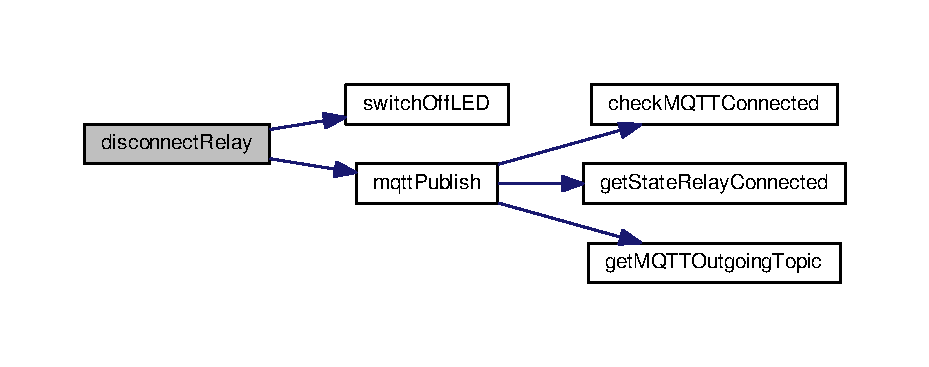
\includegraphics[width=350pt]{WIFIOnOff_8ino_ae850a8f5a550a31d8433eddf41a11d44_cgraph}
\end{center}
\end{figure}




Here is the caller graph for this function\-:
\nopagebreak
\begin{figure}[H]
\begin{center}
\leavevmode
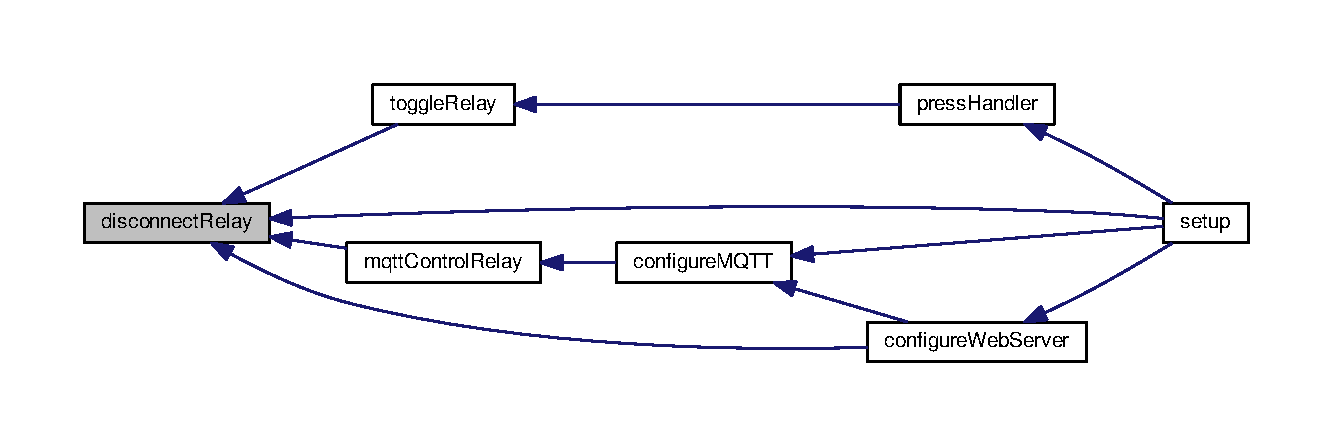
\includegraphics[width=350pt]{WIFIOnOff_8ino_ae850a8f5a550a31d8433eddf41a11d44_icgraph}
\end{center}
\end{figure}


\hypertarget{WIFIOnOff_8ino_af43969e915aec75ff3f318d585e0606a}{\index{W\-I\-F\-I\-On\-Off.\-ino@{W\-I\-F\-I\-On\-Off.\-ino}!feedback\-E\-E\-P\-R\-O\-M\-Init@{feedback\-E\-E\-P\-R\-O\-M\-Init}}
\index{feedback\-E\-E\-P\-R\-O\-M\-Init@{feedback\-E\-E\-P\-R\-O\-M\-Init}!WIFIOnOff.ino@{W\-I\-F\-I\-On\-Off.\-ino}}
\subsubsection[{feedback\-E\-E\-P\-R\-O\-M\-Init}]{\setlength{\rightskip}{0pt plus 5cm}void feedback\-E\-E\-P\-R\-O\-M\-Init (
\begin{DoxyParamCaption}
{}
\end{DoxyParamCaption}
)}}\label{WIFIOnOff_8ino_af43969e915aec75ff3f318d585e0606a}


This function is called to give the user feedback that the E\-E\-P\-R\-O\-M has been re-\//initialized. This means that all the user-\/entered data is gone and the device needs to be reconfigured. 



Here is the call graph for this function\-:
\nopagebreak
\begin{figure}[H]
\begin{center}
\leavevmode
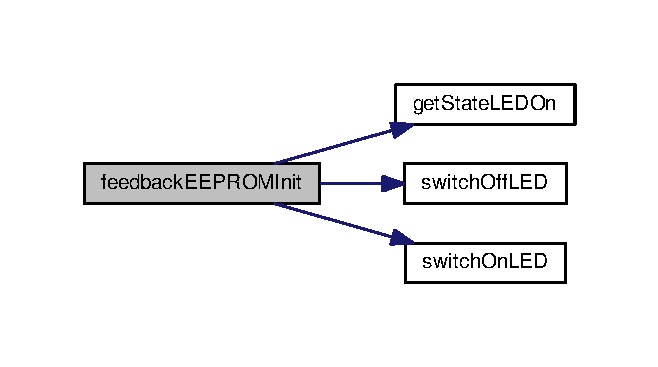
\includegraphics[width=316pt]{WIFIOnOff_8ino_af43969e915aec75ff3f318d585e0606a_cgraph}
\end{center}
\end{figure}




Here is the caller graph for this function\-:
\nopagebreak
\begin{figure}[H]
\begin{center}
\leavevmode
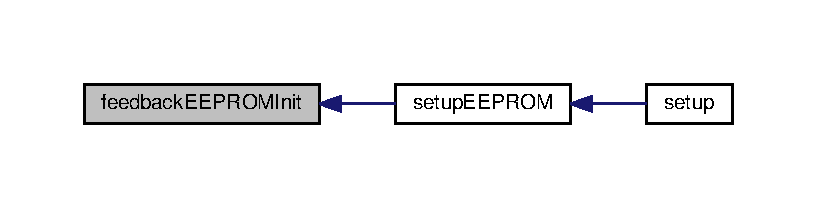
\includegraphics[width=350pt]{WIFIOnOff_8ino_af43969e915aec75ff3f318d585e0606a_icgraph}
\end{center}
\end{figure}


\hypertarget{WIFIOnOff_8ino_aed631ac5d7f4338966a6a187e1057258}{\index{W\-I\-F\-I\-On\-Off.\-ino@{W\-I\-F\-I\-On\-Off.\-ino}!feedback\-Quick\-Blink@{feedback\-Quick\-Blink}}
\index{feedback\-Quick\-Blink@{feedback\-Quick\-Blink}!WIFIOnOff.ino@{W\-I\-F\-I\-On\-Off.\-ino}}
\subsubsection[{feedback\-Quick\-Blink}]{\setlength{\rightskip}{0pt plus 5cm}void feedback\-Quick\-Blink (
\begin{DoxyParamCaption}
{}
\end{DoxyParamCaption}
)}}\label{WIFIOnOff_8ino_aed631ac5d7f4338966a6a187e1057258}


This function is called to give the user feedback about the menu the user selected. It will blink fast for a short period of time. The user has the choice to release and select the menu or to wait for the next menu. By counting the \hyperlink{WIFIOnOff_8ino_aed631ac5d7f4338966a6a187e1057258}{feedback\-Quick\-Blink()}-\/events, the user can determine which menu is selected, when the button is released now. 



Here is the call graph for this function\-:
\nopagebreak
\begin{figure}[H]
\begin{center}
\leavevmode
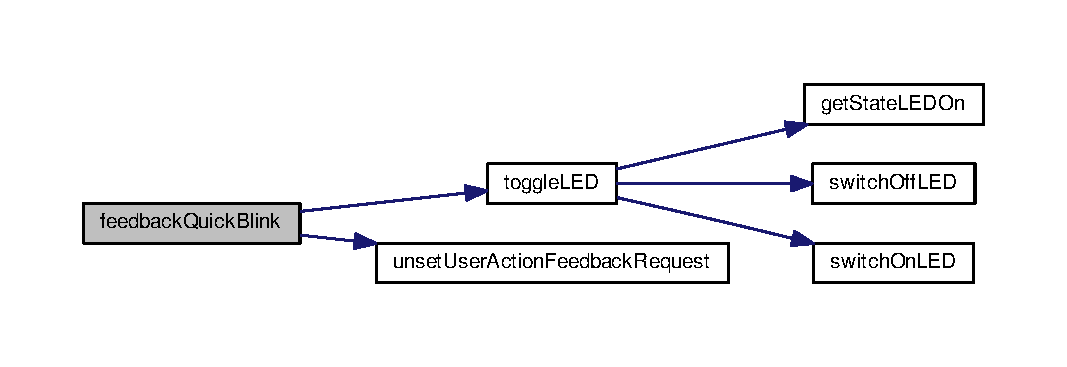
\includegraphics[width=350pt]{WIFIOnOff_8ino_aed631ac5d7f4338966a6a187e1057258_cgraph}
\end{center}
\end{figure}




Here is the caller graph for this function\-:
\nopagebreak
\begin{figure}[H]
\begin{center}
\leavevmode
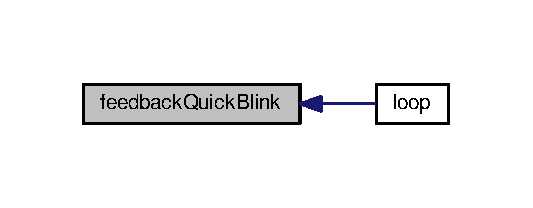
\includegraphics[width=256pt]{WIFIOnOff_8ino_aed631ac5d7f4338966a6a187e1057258_icgraph}
\end{center}
\end{figure}


\hypertarget{WIFIOnOff_8ino_a29d61ce203f552333381a79f4993da69}{\index{W\-I\-F\-I\-On\-Off.\-ino@{W\-I\-F\-I\-On\-Off.\-ino}!feedback\-W\-I\-F\-Iis\-Connecting@{feedback\-W\-I\-F\-Iis\-Connecting}}
\index{feedback\-W\-I\-F\-Iis\-Connecting@{feedback\-W\-I\-F\-Iis\-Connecting}!WIFIOnOff.ino@{W\-I\-F\-I\-On\-Off.\-ino}}
\subsubsection[{feedback\-W\-I\-F\-Iis\-Connecting}]{\setlength{\rightskip}{0pt plus 5cm}void feedback\-W\-I\-F\-Iis\-Connecting (
\begin{DoxyParamCaption}
{}
\end{DoxyParamCaption}
)}}\label{WIFIOnOff_8ino_a29d61ce203f552333381a79f4993da69}


This function is called to give the user feedback that W\-I\-F\-I is about to connect. It will blink at a medium rate. 



Here is the call graph for this function\-:
\nopagebreak
\begin{figure}[H]
\begin{center}
\leavevmode
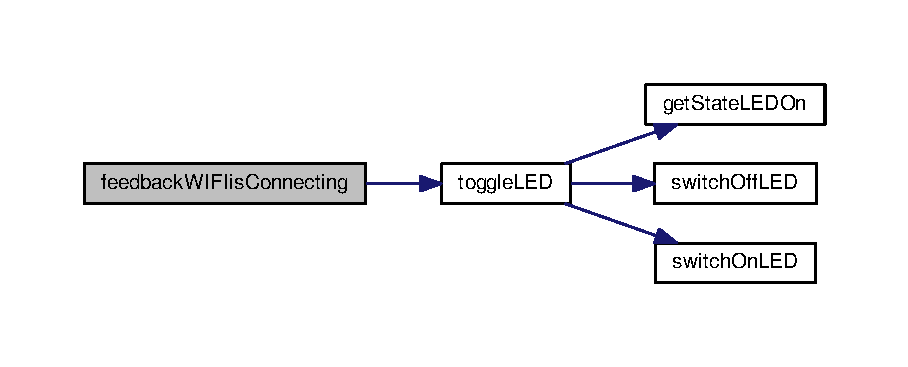
\includegraphics[width=350pt]{WIFIOnOff_8ino_a29d61ce203f552333381a79f4993da69_cgraph}
\end{center}
\end{figure}




Here is the caller graph for this function\-:
\nopagebreak
\begin{figure}[H]
\begin{center}
\leavevmode
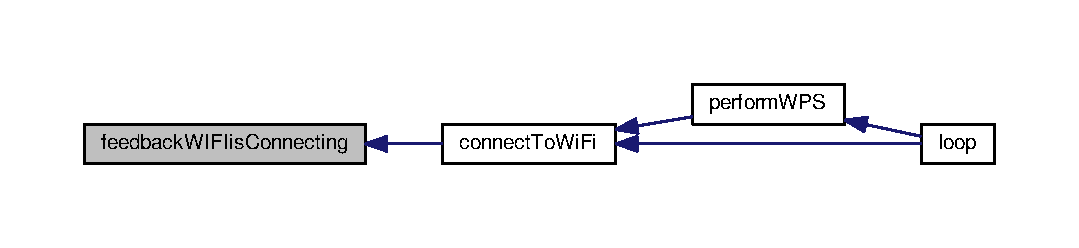
\includegraphics[width=350pt]{WIFIOnOff_8ino_a29d61ce203f552333381a79f4993da69_icgraph}
\end{center}
\end{figure}


\hypertarget{WIFIOnOff_8ino_a688bc5c57984763646a5dd2f72943255}{\index{W\-I\-F\-I\-On\-Off.\-ino@{W\-I\-F\-I\-On\-Off.\-ino}!get\-Client\-I\-D@{get\-Client\-I\-D}}
\index{get\-Client\-I\-D@{get\-Client\-I\-D}!WIFIOnOff.ino@{W\-I\-F\-I\-On\-Off.\-ino}}
\subsubsection[{get\-Client\-I\-D}]{\setlength{\rightskip}{0pt plus 5cm}String get\-Client\-I\-D (
\begin{DoxyParamCaption}
{}
\end{DoxyParamCaption}
)}}\label{WIFIOnOff_8ino_a688bc5c57984763646a5dd2f72943255}


This function returns the client name used for M\-Q\-T\-T, see \hyperlink{WIFIOnOff_8ino_a9ad5cb858c24c53a6eaa846b713bd120}{mqtt\-Connect()}. 

\begin{DoxyReturn}{Returns}
the client I\-D\-: \char`\"{}\-W\-I\-F\-I\-On\-Off\char`\"{} + M\-A\-C address 
\end{DoxyReturn}


Here is the caller graph for this function\-:
\nopagebreak
\begin{figure}[H]
\begin{center}
\leavevmode
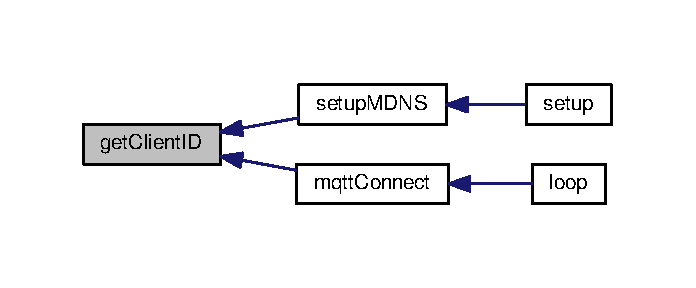
\includegraphics[width=334pt]{WIFIOnOff_8ino_a688bc5c57984763646a5dd2f72943255_icgraph}
\end{center}
\end{figure}


\hypertarget{WIFIOnOff_8ino_a3e9603214a47595af27b6e16f635734d}{\index{W\-I\-F\-I\-On\-Off.\-ino@{W\-I\-F\-I\-On\-Off.\-ino}!get\-Factory\-Reset\-Requested@{get\-Factory\-Reset\-Requested}}
\index{get\-Factory\-Reset\-Requested@{get\-Factory\-Reset\-Requested}!WIFIOnOff.ino@{W\-I\-F\-I\-On\-Off.\-ino}}
\subsubsection[{get\-Factory\-Reset\-Requested}]{\setlength{\rightskip}{0pt plus 5cm}bool get\-Factory\-Reset\-Requested (
\begin{DoxyParamCaption}
{}
\end{DoxyParamCaption}
)}}\label{WIFIOnOff_8ino_a3e9603214a47595af27b6e16f635734d}


Getter function for \hyperlink{WIFIOnOff_8ino_a4768e99cded5c5493ba789b0555c80fc}{factory\-Reset\-Requested}. 

\begin{DoxyReturn}{Returns}
true, if factory reset is requested, false otherwise. 
\end{DoxyReturn}
\hypertarget{WIFIOnOff_8ino_a92b654456d82f73760cda8b83c5a0ca6}{\index{W\-I\-F\-I\-On\-Off.\-ino@{W\-I\-F\-I\-On\-Off.\-ino}!get\-M\-Q\-T\-T\-Outgoing\-Topic@{get\-M\-Q\-T\-T\-Outgoing\-Topic}}
\index{get\-M\-Q\-T\-T\-Outgoing\-Topic@{get\-M\-Q\-T\-T\-Outgoing\-Topic}!WIFIOnOff.ino@{W\-I\-F\-I\-On\-Off.\-ino}}
\subsubsection[{get\-M\-Q\-T\-T\-Outgoing\-Topic}]{\setlength{\rightskip}{0pt plus 5cm}String get\-M\-Q\-T\-T\-Outgoing\-Topic (
\begin{DoxyParamCaption}
{}
\end{DoxyParamCaption}
)}}\label{WIFIOnOff_8ino_a92b654456d82f73760cda8b83c5a0ca6}


Getter function for \hyperlink{WIFIOnOff_8ino_a2311f2b74fe46d3f9e8072b3694deee5}{mqtt\-Outgoing\-Topic}. 

\begin{DoxyReturn}{Returns}
String of outgoing M\-Q\-T\-T topic 
\end{DoxyReturn}


Here is the caller graph for this function\-:
\nopagebreak
\begin{figure}[H]
\begin{center}
\leavevmode
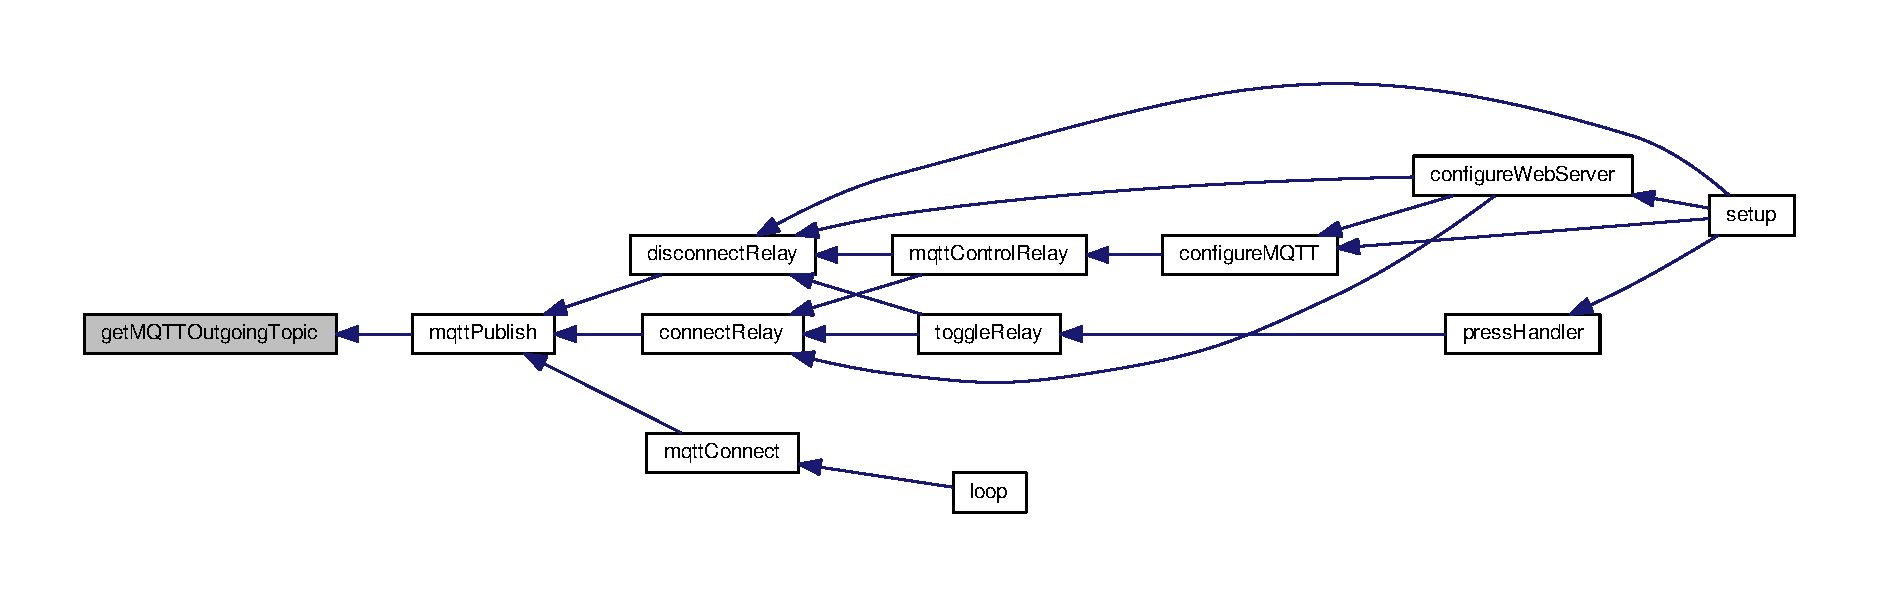
\includegraphics[width=350pt]{WIFIOnOff_8ino_a92b654456d82f73760cda8b83c5a0ca6_icgraph}
\end{center}
\end{figure}


\hypertarget{WIFIOnOff_8ino_a0914c7b7faa1375475836dc6115f1077}{\index{W\-I\-F\-I\-On\-Off.\-ino@{W\-I\-F\-I\-On\-Off.\-ino}!get\-M\-Q\-T\-T\-Server@{get\-M\-Q\-T\-T\-Server}}
\index{get\-M\-Q\-T\-T\-Server@{get\-M\-Q\-T\-T\-Server}!WIFIOnOff.ino@{W\-I\-F\-I\-On\-Off.\-ino}}
\subsubsection[{get\-M\-Q\-T\-T\-Server}]{\setlength{\rightskip}{0pt plus 5cm}String get\-M\-Q\-T\-T\-Server (
\begin{DoxyParamCaption}
{}
\end{DoxyParamCaption}
)}}\label{WIFIOnOff_8ino_a0914c7b7faa1375475836dc6115f1077}


Getter function for M\-Q\-T\-T server / broker \hyperlink{WIFIOnOff_8ino_a020889fcca6224d14f4d3f4241ca4467}{mqtt\-Server}. 

\begin{DoxyReturn}{Returns}
the latest M\-Q\-T\-T server / broker 
\end{DoxyReturn}


Here is the caller graph for this function\-:
\nopagebreak
\begin{figure}[H]
\begin{center}
\leavevmode
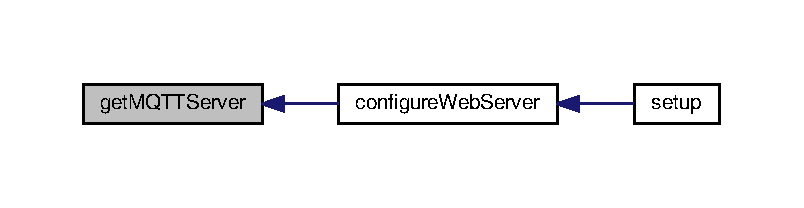
\includegraphics[width=350pt]{WIFIOnOff_8ino_a0914c7b7faa1375475836dc6115f1077_icgraph}
\end{center}
\end{figure}


\hypertarget{WIFIOnOff_8ino_af4164c2bb2661c7427bd66ecd2f8aace}{\index{W\-I\-F\-I\-On\-Off.\-ino@{W\-I\-F\-I\-On\-Off.\-ino}!get\-State\-L\-E\-D\-On@{get\-State\-L\-E\-D\-On}}
\index{get\-State\-L\-E\-D\-On@{get\-State\-L\-E\-D\-On}!WIFIOnOff.ino@{W\-I\-F\-I\-On\-Off.\-ino}}
\subsubsection[{get\-State\-L\-E\-D\-On}]{\setlength{\rightskip}{0pt plus 5cm}bool get\-State\-L\-E\-D\-On (
\begin{DoxyParamCaption}
{}
\end{DoxyParamCaption}
)}}\label{WIFIOnOff_8ino_af4164c2bb2661c7427bd66ecd2f8aace}


This function is used to get the state of the L\-E\-D. It returns \hyperlink{WIFIOnOff_8ino_aa1ef40baec048d45fac1d51afc521d40}{state\-L\-E\-D\-On}. 

\begin{DoxyReturn}{Returns}
true, if the L\-E\-D is on, false otherwise. 
\end{DoxyReturn}


Here is the caller graph for this function\-:
\nopagebreak
\begin{figure}[H]
\begin{center}
\leavevmode
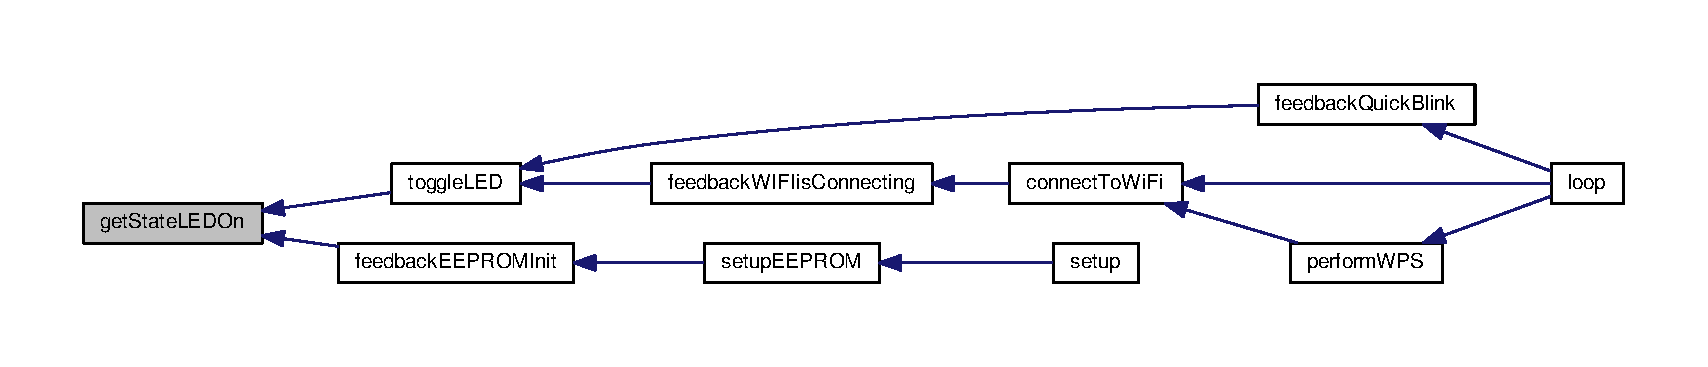
\includegraphics[width=350pt]{WIFIOnOff_8ino_af4164c2bb2661c7427bd66ecd2f8aace_icgraph}
\end{center}
\end{figure}


\hypertarget{WIFIOnOff_8ino_afc46fe517d2d628cdf59870d4f09060c}{\index{W\-I\-F\-I\-On\-Off.\-ino@{W\-I\-F\-I\-On\-Off.\-ino}!get\-State\-M\-Q\-T\-T\-Configured@{get\-State\-M\-Q\-T\-T\-Configured}}
\index{get\-State\-M\-Q\-T\-T\-Configured@{get\-State\-M\-Q\-T\-T\-Configured}!WIFIOnOff.ino@{W\-I\-F\-I\-On\-Off.\-ino}}
\subsubsection[{get\-State\-M\-Q\-T\-T\-Configured}]{\setlength{\rightskip}{0pt plus 5cm}bool get\-State\-M\-Q\-T\-T\-Configured (
\begin{DoxyParamCaption}
{}
\end{DoxyParamCaption}
)}}\label{WIFIOnOff_8ino_afc46fe517d2d628cdf59870d4f09060c}


Getter function for \hyperlink{WIFIOnOff_8ino_a3f27c574110acbefe064ca29a7ce289d}{state\-M\-Q\-T\-T\-Configured}. 

\begin{DoxyReturn}{Returns}
true if M\-Q\-T\-T is configured, false otherwise 
\end{DoxyReturn}


Here is the caller graph for this function\-:
\nopagebreak
\begin{figure}[H]
\begin{center}
\leavevmode
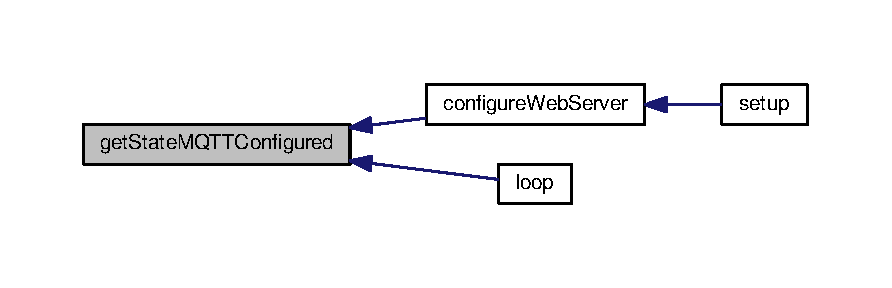
\includegraphics[width=350pt]{WIFIOnOff_8ino_afc46fe517d2d628cdf59870d4f09060c_icgraph}
\end{center}
\end{figure}


\hypertarget{WIFIOnOff_8ino_aefabc9bd763a51753669e6c249140abc}{\index{W\-I\-F\-I\-On\-Off.\-ino@{W\-I\-F\-I\-On\-Off.\-ino}!get\-State\-Relay\-Connected@{get\-State\-Relay\-Connected}}
\index{get\-State\-Relay\-Connected@{get\-State\-Relay\-Connected}!WIFIOnOff.ino@{W\-I\-F\-I\-On\-Off.\-ino}}
\subsubsection[{get\-State\-Relay\-Connected}]{\setlength{\rightskip}{0pt plus 5cm}bool get\-State\-Relay\-Connected (
\begin{DoxyParamCaption}
{}
\end{DoxyParamCaption}
)}}\label{WIFIOnOff_8ino_aefabc9bd763a51753669e6c249140abc}


This function is used to get the connection state of the relay with the mains. It returns \hyperlink{WIFIOnOff_8ino_a48a5ee80a30c37768bf1e198f1ee5692}{state\-Relay\-Connected}. 

\begin{DoxyReturn}{Returns}
true, if the relay is connected to the mains, false otherwise. 
\end{DoxyReturn}


Here is the caller graph for this function\-:
\nopagebreak
\begin{figure}[H]
\begin{center}
\leavevmode
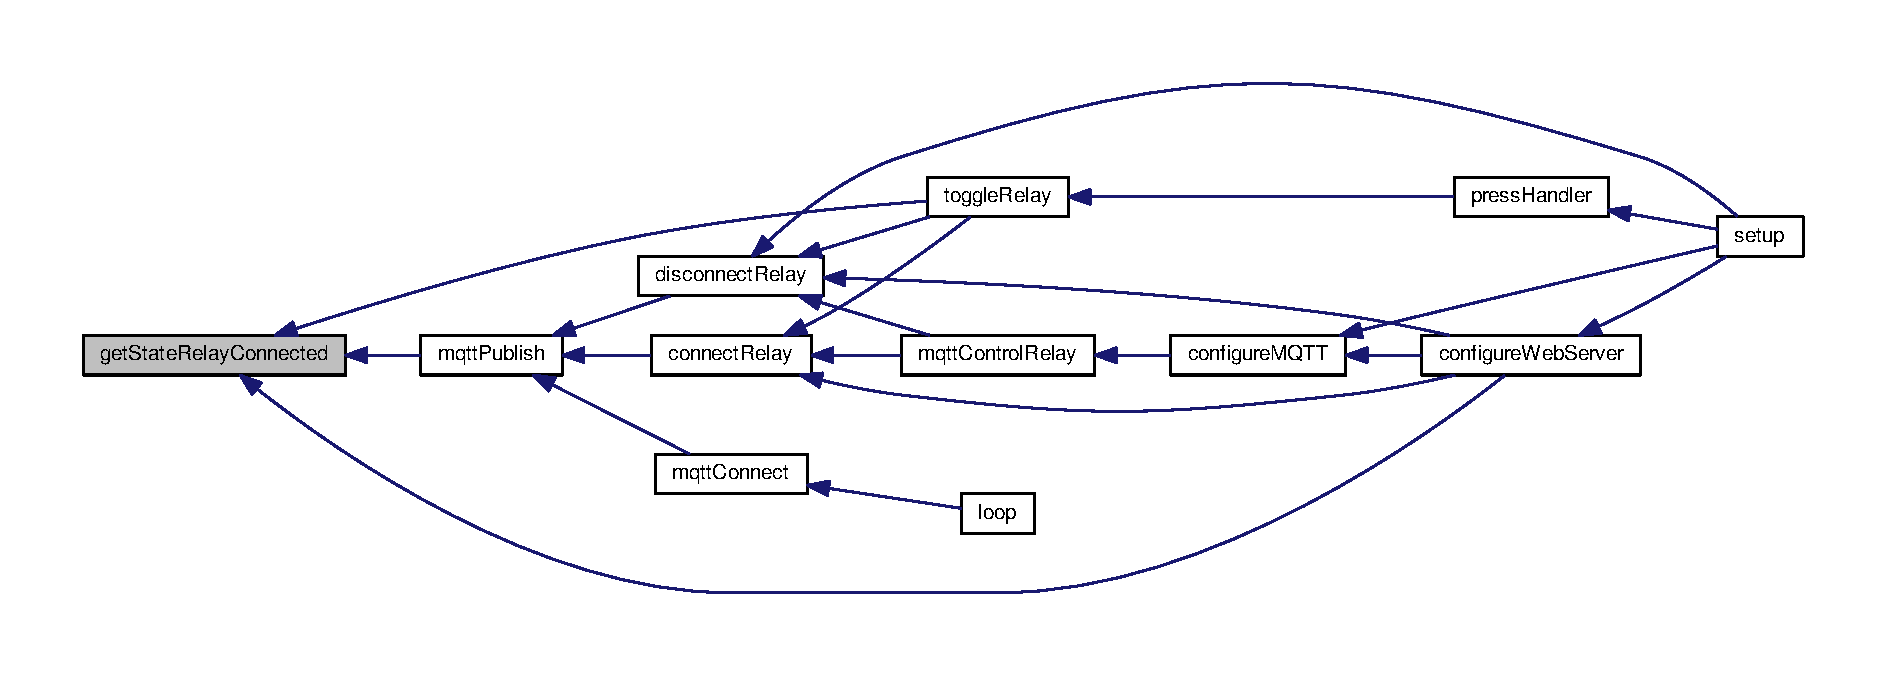
\includegraphics[width=350pt]{WIFIOnOff_8ino_aefabc9bd763a51753669e6c249140abc_icgraph}
\end{center}
\end{figure}


\hypertarget{WIFIOnOff_8ino_a347d10bac439b6c073df93cbf5522f28}{\index{W\-I\-F\-I\-On\-Off.\-ino@{W\-I\-F\-I\-On\-Off.\-ino}!get\-User\-Action\-Feedback\-Request@{get\-User\-Action\-Feedback\-Request}}
\index{get\-User\-Action\-Feedback\-Request@{get\-User\-Action\-Feedback\-Request}!WIFIOnOff.ino@{W\-I\-F\-I\-On\-Off.\-ino}}
\subsubsection[{get\-User\-Action\-Feedback\-Request}]{\setlength{\rightskip}{0pt plus 5cm}bool get\-User\-Action\-Feedback\-Request (
\begin{DoxyParamCaption}
{}
\end{DoxyParamCaption}
)}}\label{WIFIOnOff_8ino_a347d10bac439b6c073df93cbf5522f28}


Getter function for \hyperlink{WIFIOnOff_8ino_a3e5c7c27259449622535aee1125f275a}{user\-Action\-Feedback\-Request}. 

\begin{DoxyReturn}{Returns}
true, if the user should be notified that a menu can be selected, false otherwise 
\end{DoxyReturn}


Here is the caller graph for this function\-:
\nopagebreak
\begin{figure}[H]
\begin{center}
\leavevmode
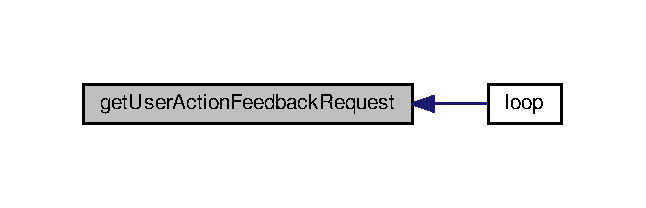
\includegraphics[width=310pt]{WIFIOnOff_8ino_a347d10bac439b6c073df93cbf5522f28_icgraph}
\end{center}
\end{figure}


\hypertarget{WIFIOnOff_8ino_aa79761488d06c15b10258afefb215020}{\index{W\-I\-F\-I\-On\-Off.\-ino@{W\-I\-F\-I\-On\-Off.\-ino}!get\-Wifi\-Reset\-Requested@{get\-Wifi\-Reset\-Requested}}
\index{get\-Wifi\-Reset\-Requested@{get\-Wifi\-Reset\-Requested}!WIFIOnOff.ino@{W\-I\-F\-I\-On\-Off.\-ino}}
\subsubsection[{get\-Wifi\-Reset\-Requested}]{\setlength{\rightskip}{0pt plus 5cm}bool get\-Wifi\-Reset\-Requested (
\begin{DoxyParamCaption}
{}
\end{DoxyParamCaption}
)}}\label{WIFIOnOff_8ino_aa79761488d06c15b10258afefb215020}


Getter function for \hyperlink{WIFIOnOff_8ino_a1ef1b3b96ca3b7c432a5c202037bcd43}{wifi\-Reset\-Requested}. 

\begin{DoxyReturn}{Returns}
true, if a deletion of W\-I\-F\-I data has been requested, false otherwise. 
\end{DoxyReturn}
\hypertarget{WIFIOnOff_8ino_a3361cdf5888fc635d5ae5d83747d50d6}{\index{W\-I\-F\-I\-On\-Off.\-ino@{W\-I\-F\-I\-On\-Off.\-ino}!get\-W\-P\-S\-Request@{get\-W\-P\-S\-Request}}
\index{get\-W\-P\-S\-Request@{get\-W\-P\-S\-Request}!WIFIOnOff.ino@{W\-I\-F\-I\-On\-Off.\-ino}}
\subsubsection[{get\-W\-P\-S\-Request}]{\setlength{\rightskip}{0pt plus 5cm}bool get\-W\-P\-S\-Request (
\begin{DoxyParamCaption}
{}
\end{DoxyParamCaption}
)}}\label{WIFIOnOff_8ino_a3361cdf5888fc635d5ae5d83747d50d6}


Getter function for \hyperlink{WIFIOnOff_8ino_a002d6cec57f207948ee9f62a3fbc12fe}{wps\-Requested}. 

\begin{DoxyReturn}{Returns}
true, if W\-P\-S has been requested, false otherwise. 
\end{DoxyReturn}
\hypertarget{WIFIOnOff_8ino_accde2e704135909387a34453e0dc1293}{\index{W\-I\-F\-I\-On\-Off.\-ino@{W\-I\-F\-I\-On\-Off.\-ino}!init\-E\-E\-P\-R\-O\-M@{init\-E\-E\-P\-R\-O\-M}}
\index{init\-E\-E\-P\-R\-O\-M@{init\-E\-E\-P\-R\-O\-M}!WIFIOnOff.ino@{W\-I\-F\-I\-On\-Off.\-ino}}
\subsubsection[{init\-E\-E\-P\-R\-O\-M}]{\setlength{\rightskip}{0pt plus 5cm}void init\-E\-E\-P\-R\-O\-M (
\begin{DoxyParamCaption}
{}
\end{DoxyParamCaption}
)}}\label{WIFIOnOff_8ino_accde2e704135909387a34453e0dc1293}


This function writes default data (\hyperlink{WIFIOnOff_8ino_a6912b1d0bb01613405a6827632e6d6f4}{E\-E\-P\-R\-O\-M\-\_\-init\-\_\-value}) to E\-E\-P\-R\-O\-M and stores C\-R\-C and the \hyperlink{WIFIOnOff_8ino_aa3109b452678c4716d01ff98ce34a2da}{E\-E\-P\-R\-O\-M\-\_\-version\-\_\-number}. 



Here is the call graph for this function\-:
\nopagebreak
\begin{figure}[H]
\begin{center}
\leavevmode
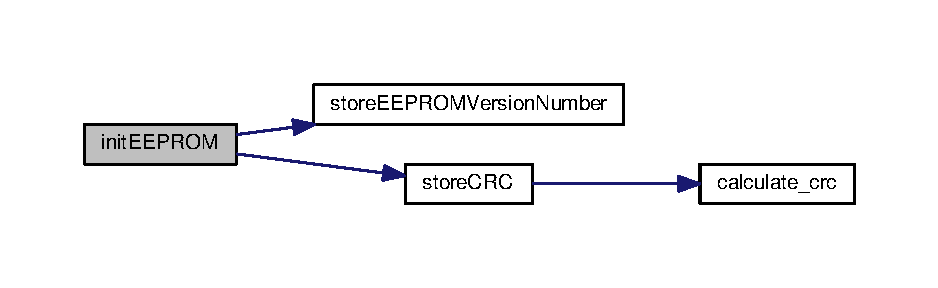
\includegraphics[width=350pt]{WIFIOnOff_8ino_accde2e704135909387a34453e0dc1293_cgraph}
\end{center}
\end{figure}




Here is the caller graph for this function\-:
\nopagebreak
\begin{figure}[H]
\begin{center}
\leavevmode
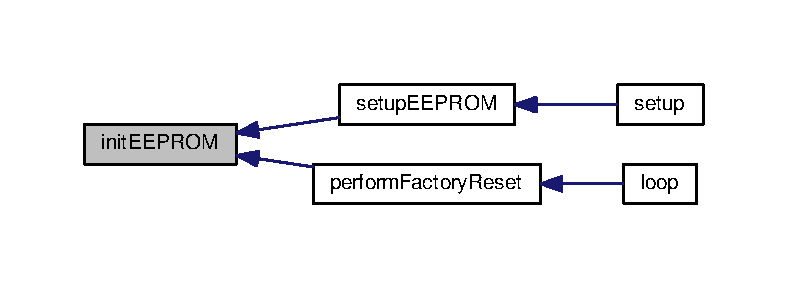
\includegraphics[width=350pt]{WIFIOnOff_8ino_accde2e704135909387a34453e0dc1293_icgraph}
\end{center}
\end{figure}


\hypertarget{WIFIOnOff_8ino_a3523db85b2f83ce089a2a733d7a025ad}{\index{W\-I\-F\-I\-On\-Off.\-ino@{W\-I\-F\-I\-On\-Off.\-ino}!is\-Not\-Whitelisted@{is\-Not\-Whitelisted}}
\index{is\-Not\-Whitelisted@{is\-Not\-Whitelisted}!WIFIOnOff.ino@{W\-I\-F\-I\-On\-Off.\-ino}}
\subsubsection[{is\-Not\-Whitelisted}]{\setlength{\rightskip}{0pt plus 5cm}bool is\-Not\-Whitelisted (
\begin{DoxyParamCaption}
\item[{char}]{c}
\end{DoxyParamCaption}
)}}\label{WIFIOnOff_8ino_a3523db85b2f83ce089a2a733d7a025ad}


This function is used for filtering out X\-S\-S attacks. This is done by whitelisting. 


\begin{DoxyItemize}
\item I\-Pv4 addresses consist of numbers and dots (0..9 $\vert$ .).
\item I\-Pv6 addresses consist of hexadeximal numbers, double dots or brackets (0..9 $\vert$ a..f $\vert$ A..F $\vert$ \mbox{[} $\vert$ \mbox{]} )
\item D\-N\-S names consist of letters, digits and hypen (0..9 $\vert$ a..z $\vert$ A..Z $\vert$ -\/ ). This function is not validating D\-N\-S, I\-Pv4, I\-Pv6. Rubbish D\-N\-S names can still pass. But characters which could be used for X\-S\-S, like $<$, $>$, \&, " are blocked. 
\begin{DoxyParams}[1]{Parameters}
\mbox{\tt in}  & {\em c} & character to check \\
\hline
\end{DoxyParams}
\begin{DoxySeeAlso}{See Also}
\href{https://www.ietf.org/rfc/rfc1035.txt}{\tt https\-://www.\-ietf.\-org/rfc/rfc1035.\-txt} 

\href{https://wonko.com/post/html-escaping}{\tt https\-://wonko.\-com/post/html-\/escaping} 

\href{https://www.owasp.org/index.php/XSS_(Cross_Site_Scripting)_Prevention_Cheat_Sheet}{\tt https\-://www.\-owasp.\-org/index.\-php/\-X\-S\-S\-\_\-(\-Cross\-\_\-\-Site\-\_\-\-Scripting)\-\_\-\-Prevention\-\_\-\-Cheat\-\_\-\-Sheet} 
\end{DoxySeeAlso}
\begin{DoxyReturn}{Returns}
true, if the argument character is not whitelisted, false otherwise. 
\end{DoxyReturn}

\end{DoxyItemize}

Here is the caller graph for this function\-:
\nopagebreak
\begin{figure}[H]
\begin{center}
\leavevmode
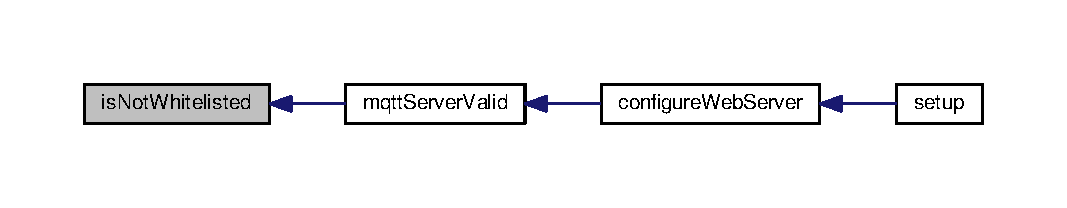
\includegraphics[width=350pt]{WIFIOnOff_8ino_a3523db85b2f83ce089a2a733d7a025ad_icgraph}
\end{center}
\end{figure}


\hypertarget{WIFIOnOff_8ino_a0b33edabd7f1c4e4a0bf32c67269be2f}{\index{W\-I\-F\-I\-On\-Off.\-ino@{W\-I\-F\-I\-On\-Off.\-ino}!loop@{loop}}
\index{loop@{loop}!WIFIOnOff.ino@{W\-I\-F\-I\-On\-Off.\-ino}}
\subsubsection[{loop}]{\setlength{\rightskip}{0pt plus 5cm}void loop (
\begin{DoxyParamCaption}
\item[{void}]{}
\end{DoxyParamCaption}
)}}\label{WIFIOnOff_8ino_a0b33edabd7f1c4e4a0bf32c67269be2f}


This function is executed in a loop after \hyperlink{WIFIOnOff_8ino_a7dfd9b79bc5a37d7df40207afbc5431f}{setup(void)} has been called. 

At first it checks for incoming user requests\-:
\begin{DoxyItemize}
\item to perform W\-P\-S (\hyperlink{WIFIOnOff_8ino_aa51eb2a71952e54dba6130be21b3a1d7}{perform\-W\-P\-S()})
\item to delete the Wi\-Fi configuration (\hyperlink{WIFIOnOff_8ino_ac782bcb28cf6c4cf77d8a408fe02c2f9}{unset\-Wi\-Fi\-Configured()})
\item to perform a factory reset (\hyperlink{WIFIOnOff_8ino_afec1c2962185272a8c87843f95d205ad}{perform\-Factory\-Reset()})
\end{DoxyItemize}

It is also checked for requests to inform the user about actions with the L\-E\-D. These requests are triggered programmatically.

After all requests are handled, it is cyclically checked that W\-P\-S has been performed and that the Wi\-Fi is connected. If W\-P\-S has not been done or Wi\-Fi is not connected, it does not make any sense to check for H\-T\-T\-P, Arduino\-O\-T\-A or M\-Q\-T\-T. For M\-Q\-T\-T to be checked, it is also required, that it was enabled by the user.

If M\-Q\-T\-T is not connected, try to connect, otherwise handle M\-Q\-T\-T. 

Here is the call graph for this function\-:
\nopagebreak
\begin{figure}[H]
\begin{center}
\leavevmode
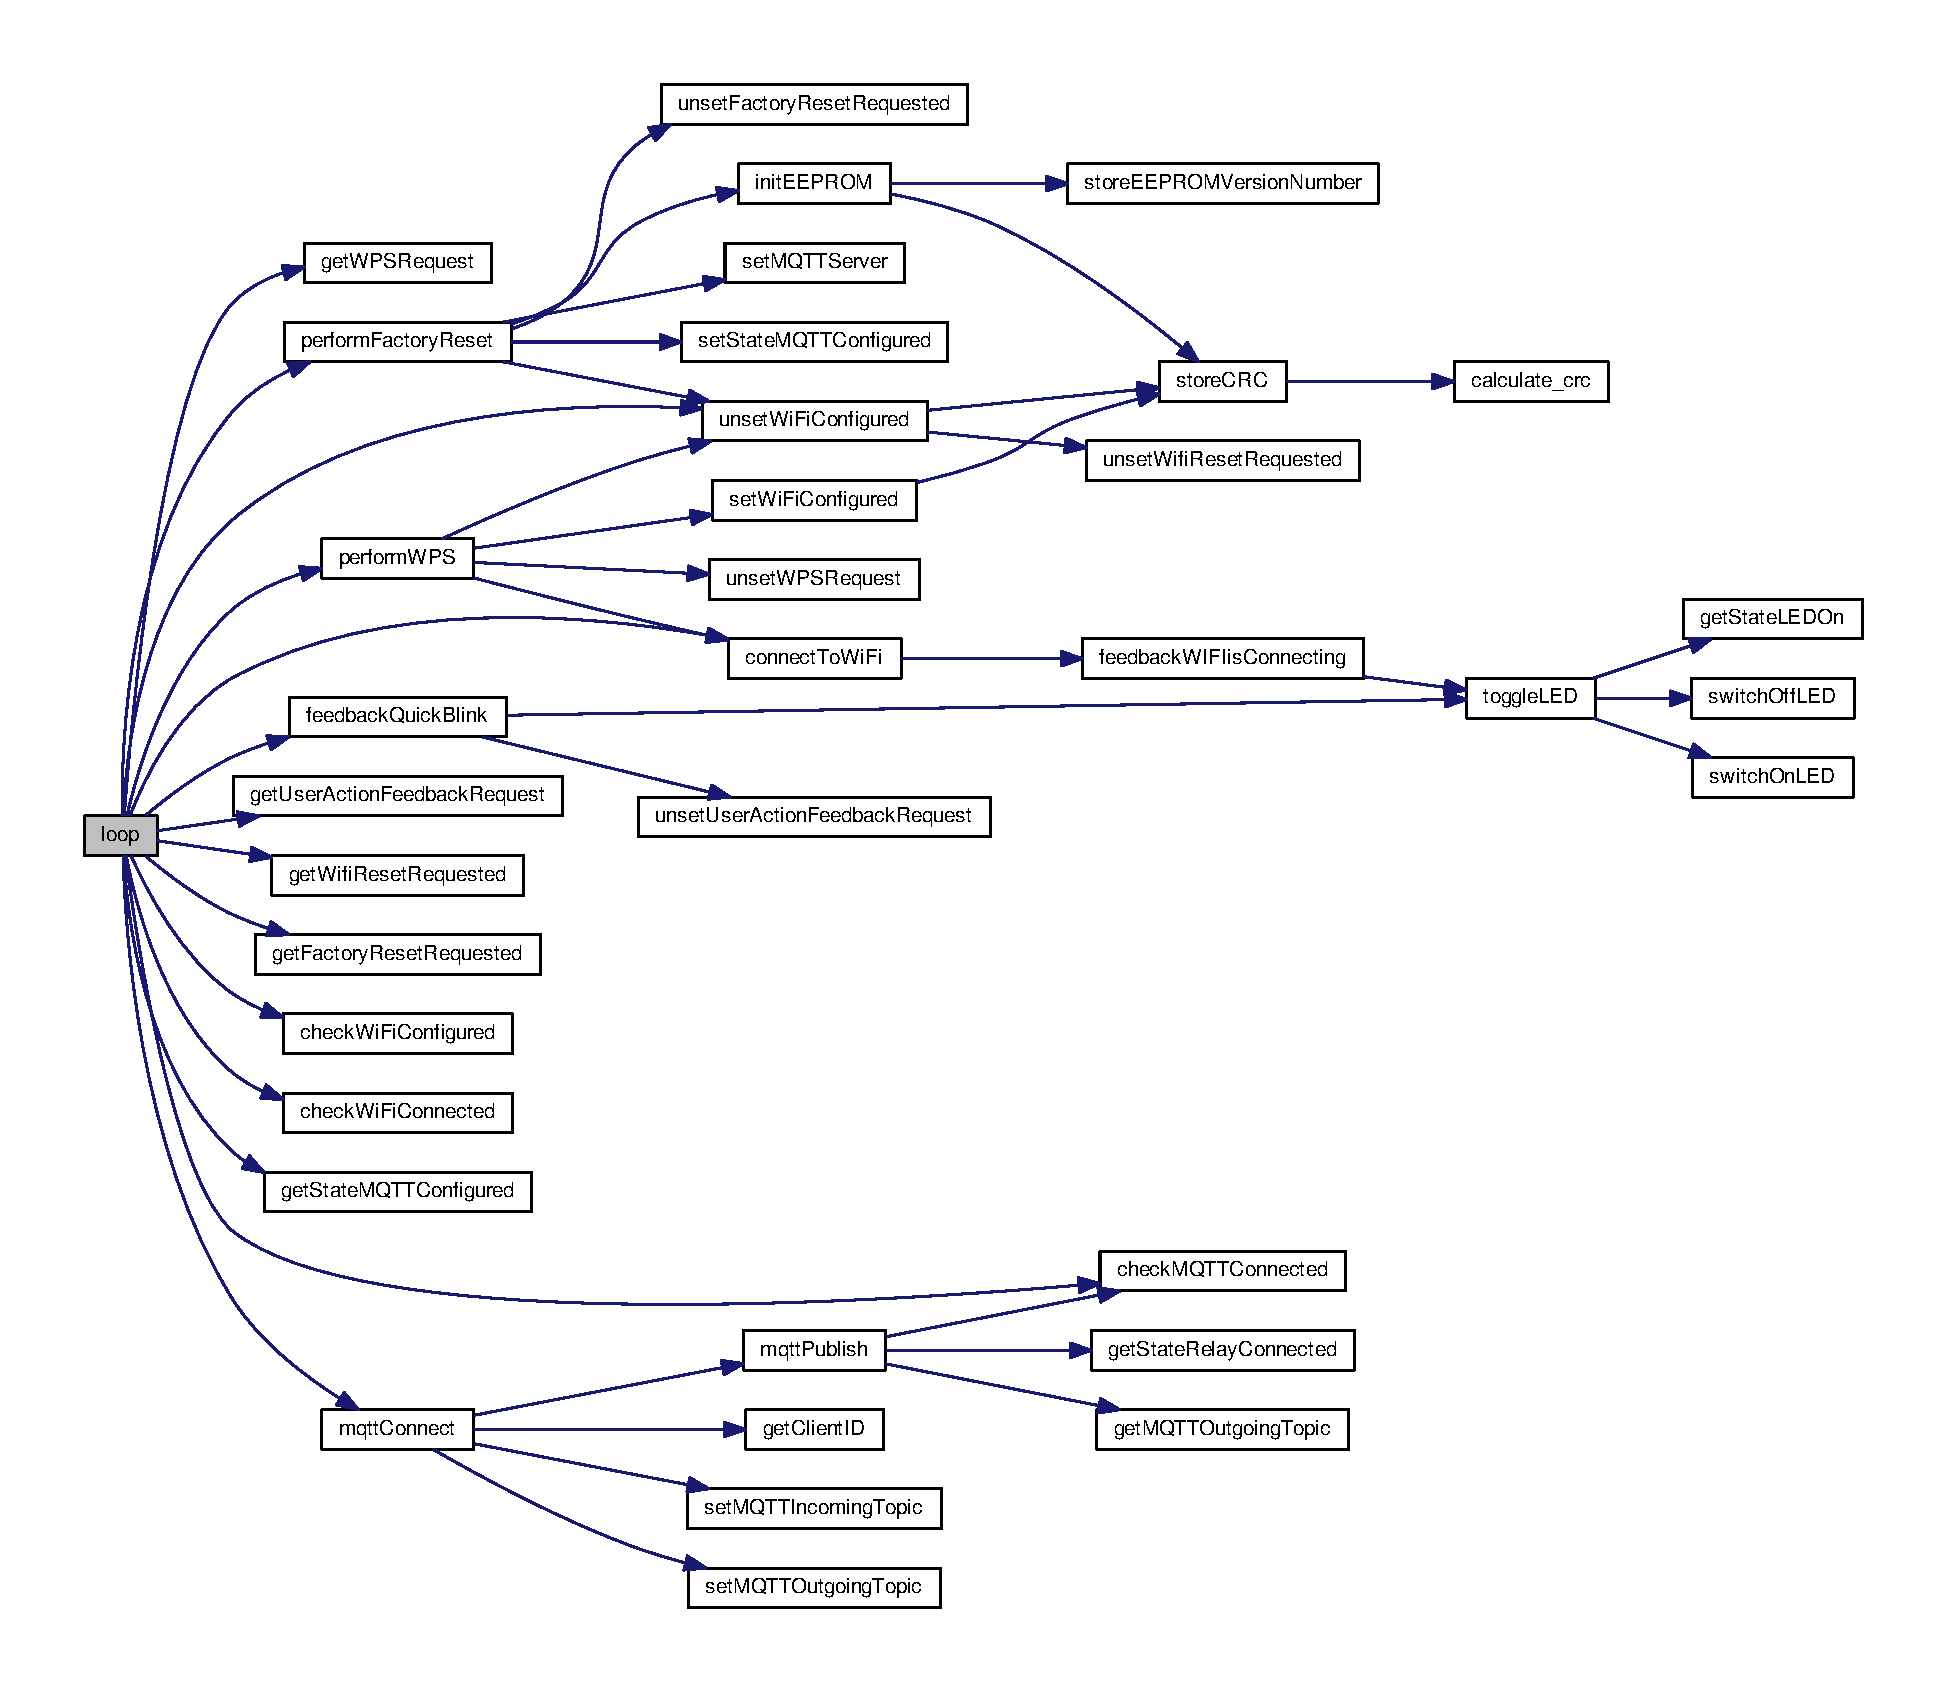
\includegraphics[width=350pt]{WIFIOnOff_8ino_a0b33edabd7f1c4e4a0bf32c67269be2f_cgraph}
\end{center}
\end{figure}


\hypertarget{WIFIOnOff_8ino_a9ad5cb858c24c53a6eaa846b713bd120}{\index{W\-I\-F\-I\-On\-Off.\-ino@{W\-I\-F\-I\-On\-Off.\-ino}!mqtt\-Connect@{mqtt\-Connect}}
\index{mqtt\-Connect@{mqtt\-Connect}!WIFIOnOff.ino@{W\-I\-F\-I\-On\-Off.\-ino}}
\subsubsection[{mqtt\-Connect}]{\setlength{\rightskip}{0pt plus 5cm}void mqtt\-Connect (
\begin{DoxyParamCaption}
{}
\end{DoxyParamCaption}
)}}\label{WIFIOnOff_8ino_a9ad5cb858c24c53a6eaa846b713bd120}


This function connects to broker and. 


\begin{DoxyItemize}
\item subscribes topic wifionoff/get\-Client\-I\-D()/set
\item sets last will \char`\"{}disconnected\char`\"{} on wifionoff/get\-Client\-I\-D()/get
\item publishes latest state on wifionoff/get\-Client\-I\-D()/get 
\end{DoxyItemize}

Here is the call graph for this function\-:
\nopagebreak
\begin{figure}[H]
\begin{center}
\leavevmode
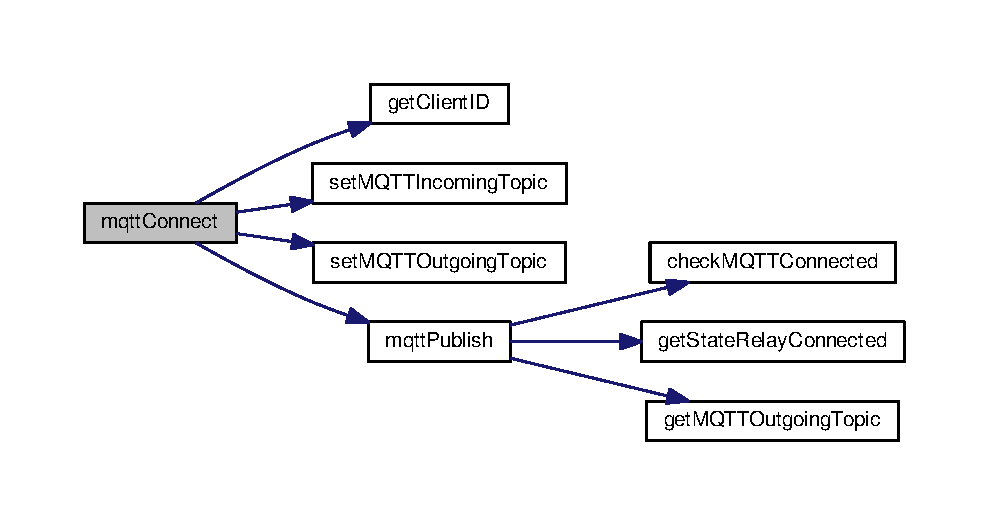
\includegraphics[width=350pt]{WIFIOnOff_8ino_a9ad5cb858c24c53a6eaa846b713bd120_cgraph}
\end{center}
\end{figure}




Here is the caller graph for this function\-:
\nopagebreak
\begin{figure}[H]
\begin{center}
\leavevmode
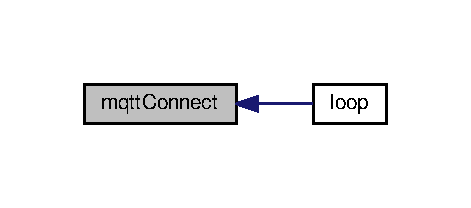
\includegraphics[width=226pt]{WIFIOnOff_8ino_a9ad5cb858c24c53a6eaa846b713bd120_icgraph}
\end{center}
\end{figure}


\hypertarget{WIFIOnOff_8ino_ab913592c54bd79feda56cbdc86f44641}{\index{W\-I\-F\-I\-On\-Off.\-ino@{W\-I\-F\-I\-On\-Off.\-ino}!mqtt\-Control\-Relay@{mqtt\-Control\-Relay}}
\index{mqtt\-Control\-Relay@{mqtt\-Control\-Relay}!WIFIOnOff.ino@{W\-I\-F\-I\-On\-Off.\-ino}}
\subsubsection[{mqtt\-Control\-Relay}]{\setlength{\rightskip}{0pt plus 5cm}void mqtt\-Control\-Relay (
\begin{DoxyParamCaption}
\item[{String \&}]{topic, }
\item[{String \&}]{payload}
\end{DoxyParamCaption}
)}}\label{WIFIOnOff_8ino_ab913592c54bd79feda56cbdc86f44641}


Callback which is called when M\-Q\-T\-T receives an incoming topic. 


\begin{DoxyParams}[1]{Parameters}
\mbox{\tt in}  & {\em topic} & One of the incoming M\-Q\-T\-T topics, which the \hyperlink{WIFIOnOff_8ino_a0524591f2a058a4f26f16579245db356}{mqtt\-Client} has been subscribed to. Currently there is only one connection, see \hyperlink{WIFIOnOff_8ino_a9ad5cb858c24c53a6eaa846b713bd120}{mqtt\-Connect()}. So this parameter is irrelevant. \\
\hline
\mbox{\tt in}  & {\em payload} & Contains the received payload of the message of the incoming topic. If \char`\"{}on\char`\"{} or \char`\"{}1\char`\"{} is received, the relay is connected (\hyperlink{WIFIOnOff_8ino_a6eda13f766d5d36ba8bcbe7c252c2ab8}{connect\-Relay()}), else if \char`\"{}off\char`\"{} or \char`\"{}0\char`\"{} is received, the relay is disconnected (\hyperlink{WIFIOnOff_8ino_ae850a8f5a550a31d8433eddf41a11d44}{disconnect\-Relay()}). \\
\hline
\end{DoxyParams}


Here is the call graph for this function\-:
\nopagebreak
\begin{figure}[H]
\begin{center}
\leavevmode
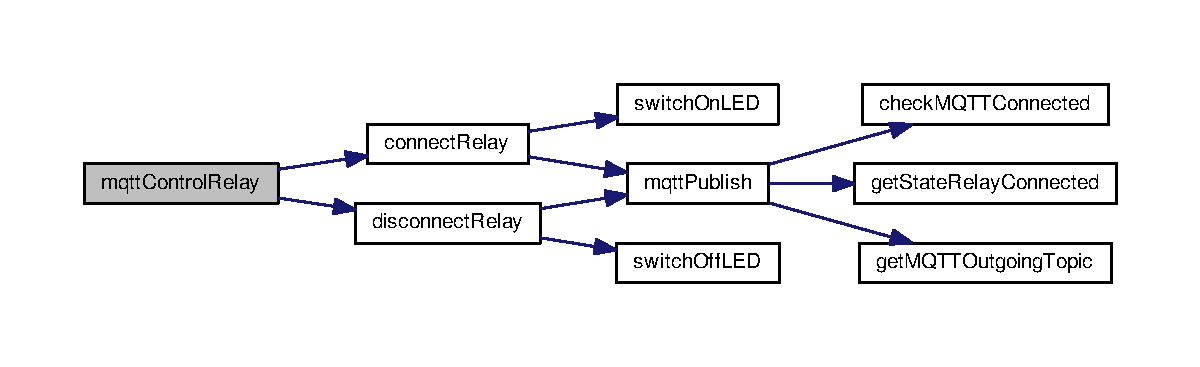
\includegraphics[width=350pt]{WIFIOnOff_8ino_ab913592c54bd79feda56cbdc86f44641_cgraph}
\end{center}
\end{figure}




Here is the caller graph for this function\-:
\nopagebreak
\begin{figure}[H]
\begin{center}
\leavevmode
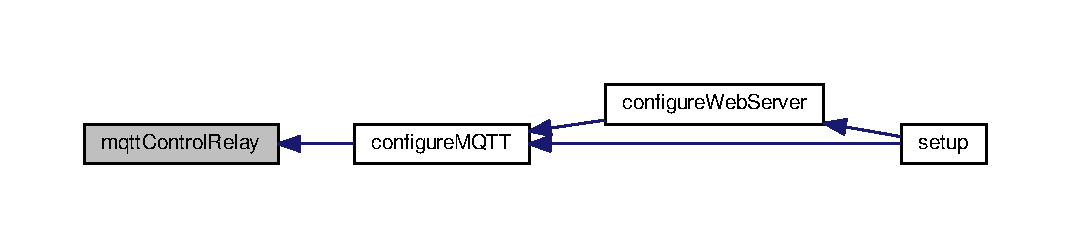
\includegraphics[width=350pt]{WIFIOnOff_8ino_ab913592c54bd79feda56cbdc86f44641_icgraph}
\end{center}
\end{figure}


\hypertarget{WIFIOnOff_8ino_a92e8e72a8c9bd699aefa63b65c4bc30c}{\index{W\-I\-F\-I\-On\-Off.\-ino@{W\-I\-F\-I\-On\-Off.\-ino}!mqtt\-Publish@{mqtt\-Publish}}
\index{mqtt\-Publish@{mqtt\-Publish}!WIFIOnOff.ino@{W\-I\-F\-I\-On\-Off.\-ino}}
\subsubsection[{mqtt\-Publish}]{\setlength{\rightskip}{0pt plus 5cm}void mqtt\-Publish (
\begin{DoxyParamCaption}
{}
\end{DoxyParamCaption}
)}}\label{WIFIOnOff_8ino_a92e8e72a8c9bd699aefa63b65c4bc30c}


With the call of this function, \hyperlink{WIFIOnOff_8ino_a0524591f2a058a4f26f16579245db356}{mqtt\-Client} publishes the state of the relay (\hyperlink{WIFIOnOff_8ino_aefabc9bd763a51753669e6c249140abc}{get\-State\-Relay\-Connected()}) on the outgoing topic (\hyperlink{WIFIOnOff_8ino_a92b654456d82f73760cda8b83c5a0ca6}{get\-M\-Q\-T\-T\-Outgoing\-Topic()}) to the M\-Q\-T\-T server / broker. The macro \hyperlink{WIFIOnOff_8ino_a59912dabf54ca43542cdc292e80d5742}{N\-U\-M\-E\-R\-I\-C\-\_\-\-R\-E\-S\-P\-O\-N\-S\-E} is taken into account. 



Here is the call graph for this function\-:
\nopagebreak
\begin{figure}[H]
\begin{center}
\leavevmode
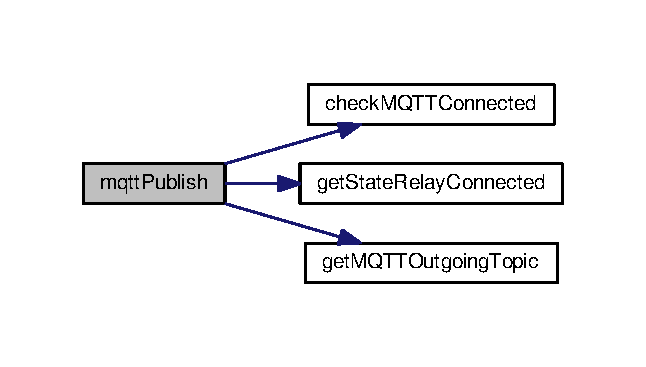
\includegraphics[width=310pt]{WIFIOnOff_8ino_a92e8e72a8c9bd699aefa63b65c4bc30c_cgraph}
\end{center}
\end{figure}




Here is the caller graph for this function\-:
\nopagebreak
\begin{figure}[H]
\begin{center}
\leavevmode
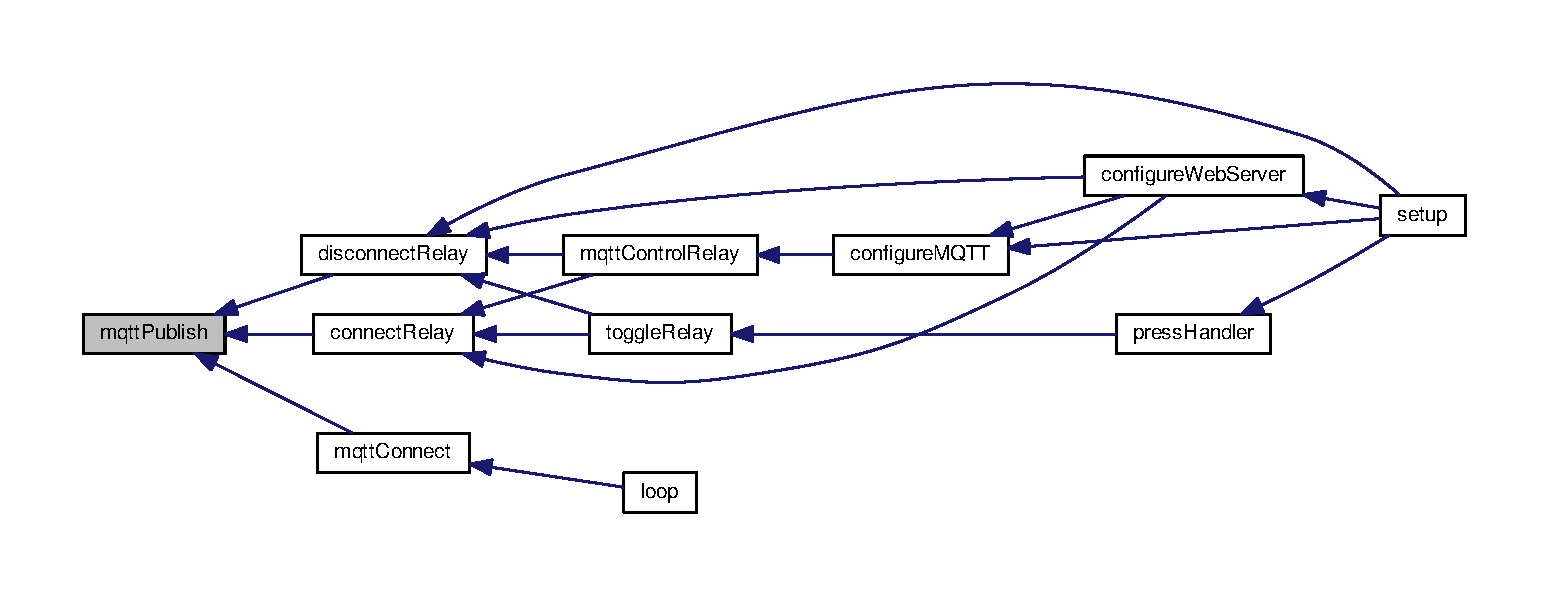
\includegraphics[width=350pt]{WIFIOnOff_8ino_a92e8e72a8c9bd699aefa63b65c4bc30c_icgraph}
\end{center}
\end{figure}


\hypertarget{WIFIOnOff_8ino_a3251df1e6168789bae584b4063d5a59d}{\index{W\-I\-F\-I\-On\-Off.\-ino@{W\-I\-F\-I\-On\-Off.\-ino}!mqtt\-Server\-Valid@{mqtt\-Server\-Valid}}
\index{mqtt\-Server\-Valid@{mqtt\-Server\-Valid}!WIFIOnOff.ino@{W\-I\-F\-I\-On\-Off.\-ino}}
\subsubsection[{mqtt\-Server\-Valid}]{\setlength{\rightskip}{0pt plus 5cm}bool mqtt\-Server\-Valid (
\begin{DoxyParamCaption}
\item[{String}]{mqtt\-Server}
\end{DoxyParamCaption}
)}}\label{WIFIOnOff_8ino_a3251df1e6168789bae584b4063d5a59d}


This function is used to check whether mqtt\-Server is valid. Therefore, it is checked that the. 


\begin{DoxyItemize}
\item length of mqtt\-Server is less or equal than \hyperlink{WIFIOnOff_8ino_ac060eafb02eba00d33cad29f38819d4a}{E\-E\-P\-R\-O\-M\-\_\-size\-\_\-\-M\-Q\-T\-T\-\_\-server}
\item all characters are whitelisted (see \hyperlink{WIFIOnOff_8ino_a3523db85b2f83ce089a2a733d7a025ad}{is\-Not\-Whitelisted()}) 
\begin{DoxyParams}[1]{Parameters}
\mbox{\tt in}  & {\em mqtt\-Server} & String to check for validity \\
\hline
\end{DoxyParams}
\begin{DoxyReturn}{Returns}
true, if mqtt\-Server is valid, false otherwise. 
\end{DoxyReturn}

\end{DoxyItemize}

Here is the call graph for this function\-:
\nopagebreak
\begin{figure}[H]
\begin{center}
\leavevmode
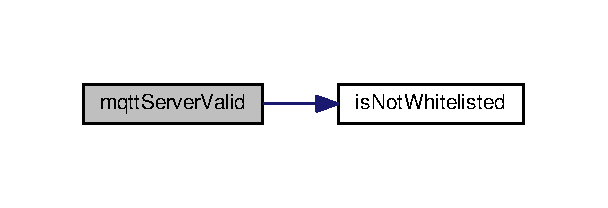
\includegraphics[width=292pt]{WIFIOnOff_8ino_a3251df1e6168789bae584b4063d5a59d_cgraph}
\end{center}
\end{figure}




Here is the caller graph for this function\-:
\nopagebreak
\begin{figure}[H]
\begin{center}
\leavevmode
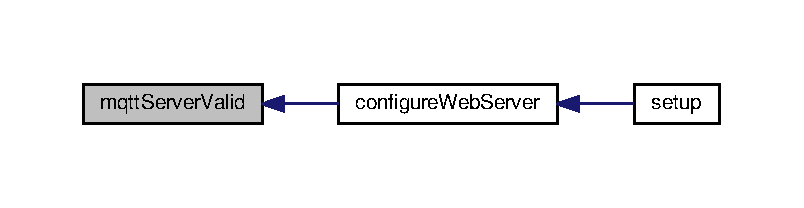
\includegraphics[width=350pt]{WIFIOnOff_8ino_a3251df1e6168789bae584b4063d5a59d_icgraph}
\end{center}
\end{figure}


\hypertarget{WIFIOnOff_8ino_afec1c2962185272a8c87843f95d205ad}{\index{W\-I\-F\-I\-On\-Off.\-ino@{W\-I\-F\-I\-On\-Off.\-ino}!perform\-Factory\-Reset@{perform\-Factory\-Reset}}
\index{perform\-Factory\-Reset@{perform\-Factory\-Reset}!WIFIOnOff.ino@{W\-I\-F\-I\-On\-Off.\-ino}}
\subsubsection[{perform\-Factory\-Reset}]{\setlength{\rightskip}{0pt plus 5cm}void perform\-Factory\-Reset (
\begin{DoxyParamCaption}
{}
\end{DoxyParamCaption}
)}}\label{WIFIOnOff_8ino_afec1c2962185272a8c87843f95d205ad}


Perform factory reset. 


\begin{DoxyItemize}
\item reset Wi\-Fi
\item reset M\-Q\-T\-T
\item reset E\-E\-P\-R\-O\-M 
\end{DoxyItemize}

Here is the call graph for this function\-:
\nopagebreak
\begin{figure}[H]
\begin{center}
\leavevmode
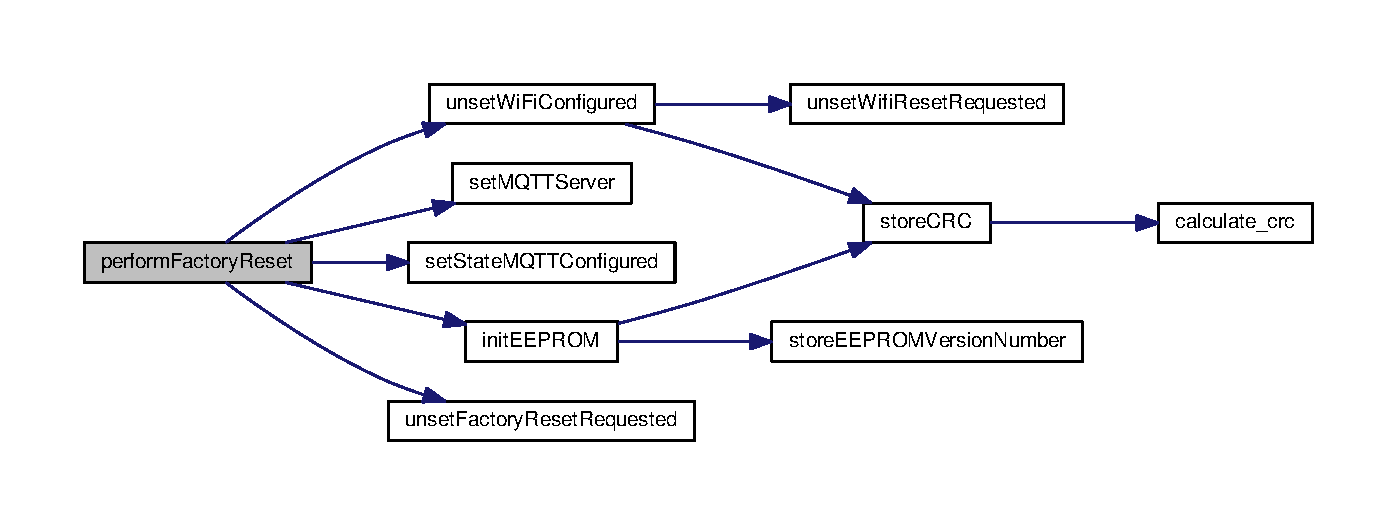
\includegraphics[width=350pt]{WIFIOnOff_8ino_afec1c2962185272a8c87843f95d205ad_cgraph}
\end{center}
\end{figure}




Here is the caller graph for this function\-:
\nopagebreak
\begin{figure}[H]
\begin{center}
\leavevmode
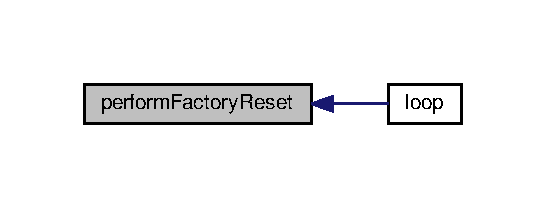
\includegraphics[width=262pt]{WIFIOnOff_8ino_afec1c2962185272a8c87843f95d205ad_icgraph}
\end{center}
\end{figure}


\hypertarget{WIFIOnOff_8ino_aa51eb2a71952e54dba6130be21b3a1d7}{\index{W\-I\-F\-I\-On\-Off.\-ino@{W\-I\-F\-I\-On\-Off.\-ino}!perform\-W\-P\-S@{perform\-W\-P\-S}}
\index{perform\-W\-P\-S@{perform\-W\-P\-S}!WIFIOnOff.ino@{W\-I\-F\-I\-On\-Off.\-ino}}
\subsubsection[{perform\-W\-P\-S}]{\setlength{\rightskip}{0pt plus 5cm}void perform\-W\-P\-S (
\begin{DoxyParamCaption}
{}
\end{DoxyParamCaption}
)}}\label{WIFIOnOff_8ino_aa51eb2a71952e54dba6130be21b3a1d7}


This function is used to trigger W\-P\-S. If W\-P\-S has been successful, \hyperlink{WIFIOnOff_8ino_a3ebcee2a9d20137810223c6813e54787}{set\-Wi\-Fi\-Configured()} is executed and \hyperlink{WIFIOnOff_8ino_a86eebd69aeee5bbb5e648fc099b4b360}{unset\-W\-P\-S\-Request()} is called. 



Here is the call graph for this function\-:
\nopagebreak
\begin{figure}[H]
\begin{center}
\leavevmode
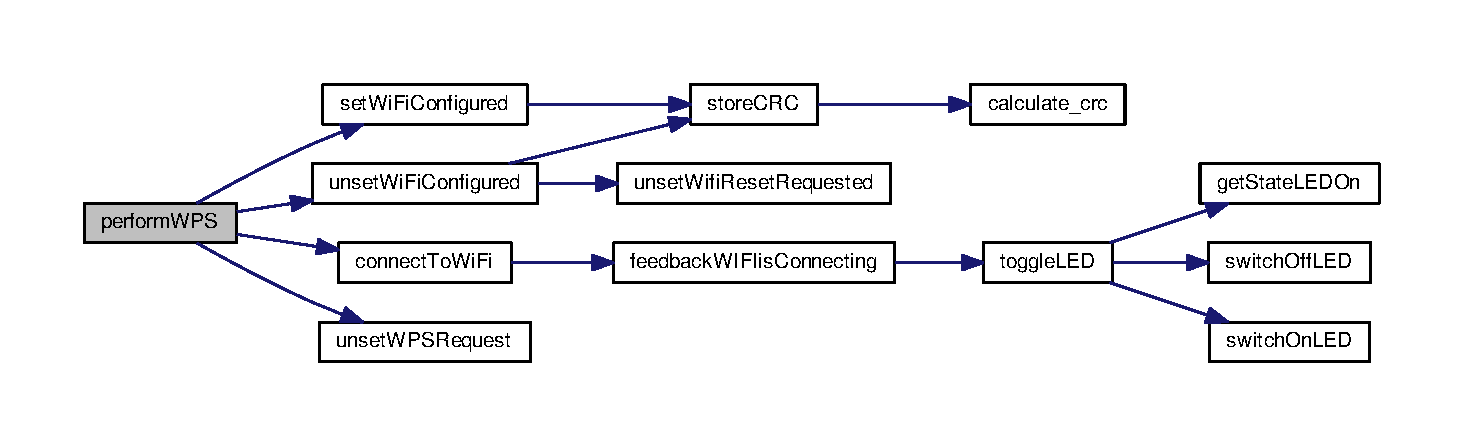
\includegraphics[width=350pt]{WIFIOnOff_8ino_aa51eb2a71952e54dba6130be21b3a1d7_cgraph}
\end{center}
\end{figure}




Here is the caller graph for this function\-:
\nopagebreak
\begin{figure}[H]
\begin{center}
\leavevmode
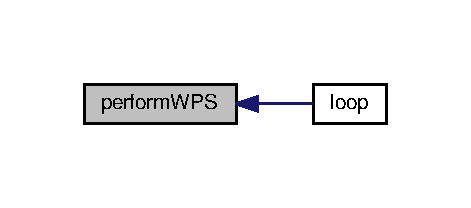
\includegraphics[width=226pt]{WIFIOnOff_8ino_aa51eb2a71952e54dba6130be21b3a1d7_icgraph}
\end{center}
\end{figure}


\hypertarget{WIFIOnOff_8ino_acd4d58af93c899ee9a03131727b1cf34}{\index{W\-I\-F\-I\-On\-Off.\-ino@{W\-I\-F\-I\-On\-Off.\-ino}!press\-Handler@{press\-Handler}}
\index{press\-Handler@{press\-Handler}!WIFIOnOff.ino@{W\-I\-F\-I\-On\-Off.\-ino}}
\subsubsection[{press\-Handler}]{\setlength{\rightskip}{0pt plus 5cm}void press\-Handler (
\begin{DoxyParamCaption}
{}
\end{DoxyParamCaption}
)}}\label{WIFIOnOff_8ino_acd4d58af93c899ee9a03131727b1cf34}


This function triggers. 


\begin{DoxyItemize}
\item the toggling of the relay
\item W\-P\-S button method request
\item factory reset request. As this function is called regularly with \hyperlink{WIFIOnOff_8ino_a4bb2542b2738619fdf76b685b10e315d}{ticker}, it should be quick, otherwise the E\-S\-P8266 might crash. \begin{DoxySeeAlso}{See Also}
\href{https://arduino-esp8266.readthedocs.io/en/latest/faq/a02-my-esp-crashes.html}{\tt https\-://arduino-\/esp8266.\-readthedocs.\-io/en/latest/faq/a02-\/my-\/esp-\/crashes.\-html} 
\end{DoxySeeAlso}

\end{DoxyItemize}

Here is the call graph for this function\-:
\nopagebreak
\begin{figure}[H]
\begin{center}
\leavevmode
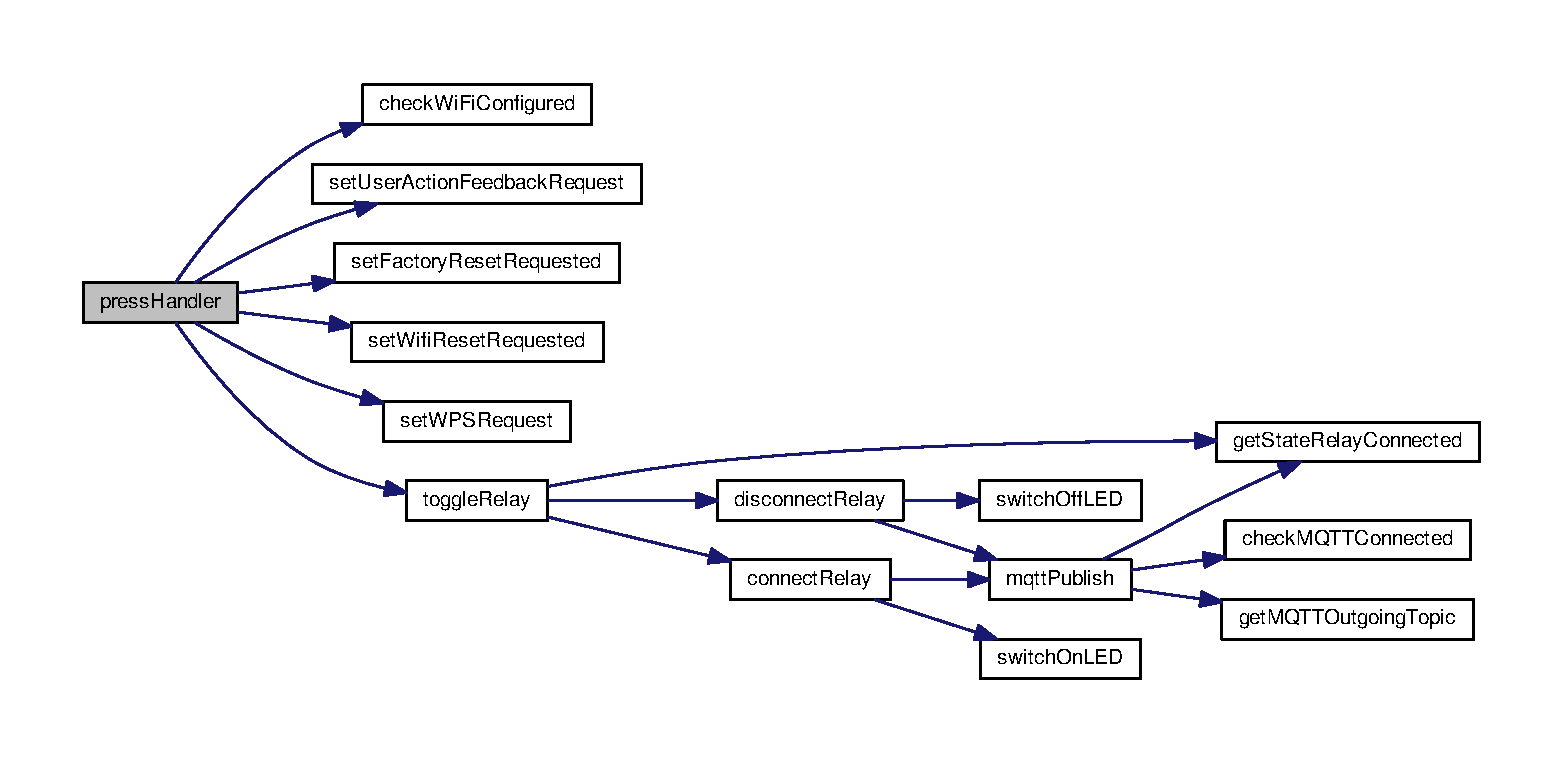
\includegraphics[width=350pt]{WIFIOnOff_8ino_acd4d58af93c899ee9a03131727b1cf34_cgraph}
\end{center}
\end{figure}




Here is the caller graph for this function\-:
\nopagebreak
\begin{figure}[H]
\begin{center}
\leavevmode
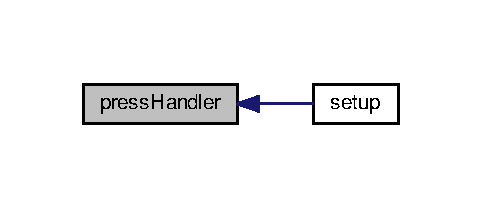
\includegraphics[width=232pt]{WIFIOnOff_8ino_acd4d58af93c899ee9a03131727b1cf34_icgraph}
\end{center}
\end{figure}


\hypertarget{WIFIOnOff_8ino_a12a8bd3c3a1288633c3eade6ee8e77cf}{\index{W\-I\-F\-I\-On\-Off.\-ino@{W\-I\-F\-I\-On\-Off.\-ino}!render\-Footer@{render\-Footer}}
\index{render\-Footer@{render\-Footer}!WIFIOnOff.ino@{W\-I\-F\-I\-On\-Off.\-ino}}
\subsubsection[{render\-Footer}]{\setlength{\rightskip}{0pt plus 5cm}String render\-Footer (
\begin{DoxyParamCaption}
{}
\end{DoxyParamCaption}
)}}\label{WIFIOnOff_8ino_a12a8bd3c3a1288633c3eade6ee8e77cf}


This function returns the last part of a H\-T\-M\-L file which is reused for all responses. 

\begin{DoxyReturn}{Returns}
\char`\"{}$<$/body$>$$<$/html$>$\char`\"{}, look inside the function for more information. 
\end{DoxyReturn}


Here is the caller graph for this function\-:
\nopagebreak
\begin{figure}[H]
\begin{center}
\leavevmode
\includegraphics[width=350pt]{WIFIOnOff_8ino_a12a8bd3c3a1288633c3eade6ee8e77cf_icgraph}
\end{center}
\end{figure}


\hypertarget{WIFIOnOff_8ino_a1ec8a91d3b174c2cfee9eaf852f11c1e}{\index{W\-I\-F\-I\-On\-Off.\-ino@{W\-I\-F\-I\-On\-Off.\-ino}!render\-Header@{render\-Header}}
\index{render\-Header@{render\-Header}!WIFIOnOff.ino@{W\-I\-F\-I\-On\-Off.\-ino}}
\subsubsection[{render\-Header}]{\setlength{\rightskip}{0pt plus 5cm}String render\-Header (
\begin{DoxyParamCaption}
{}
\end{DoxyParamCaption}
)}}\label{WIFIOnOff_8ino_a1ec8a91d3b174c2cfee9eaf852f11c1e}


This function returns the first part of a H\-T\-M\-L file which is reused for all responses. 

\begin{DoxyReturn}{Returns}
\char`\"{}$<$!doctype$>$ ... $<$body$>$\char`\"{}, look inside the function for more information. 
\end{DoxyReturn}
\begin{DoxySeeAlso}{See Also}
\href{http://www.html.am/templates/css-templates/}{\tt http\-://www.\-html.\-am/templates/css-\/templates/} 
\end{DoxySeeAlso}


Here is the caller graph for this function\-:
\nopagebreak
\begin{figure}[H]
\begin{center}
\leavevmode
\includegraphics[width=350pt]{WIFIOnOff_8ino_a1ec8a91d3b174c2cfee9eaf852f11c1e_icgraph}
\end{center}
\end{figure}


\hypertarget{WIFIOnOff_8ino_a4dfcb1cefe2bee38d172e3f327c1a72d}{\index{W\-I\-F\-I\-On\-Off.\-ino@{W\-I\-F\-I\-On\-Off.\-ino}!render\-M\-Q\-T\-T\-Server\-Settings@{render\-M\-Q\-T\-T\-Server\-Settings}}
\index{render\-M\-Q\-T\-T\-Server\-Settings@{render\-M\-Q\-T\-T\-Server\-Settings}!WIFIOnOff.ino@{W\-I\-F\-I\-On\-Off.\-ino}}
\subsubsection[{render\-M\-Q\-T\-T\-Server\-Settings}]{\setlength{\rightskip}{0pt plus 5cm}String render\-M\-Q\-T\-T\-Server\-Settings (
\begin{DoxyParamCaption}
\item[{String}]{stored\-Server\-Name, }
\item[{String}]{failure\-Msg, }
\item[{bool}]{state\-M\-Q\-T\-T\-Activated, }
\item[{bool}]{state\-M\-Q\-T\-T\-Connected}
\end{DoxyParamCaption}
)}}\label{WIFIOnOff_8ino_a4dfcb1cefe2bee38d172e3f327c1a72d}


This function returns the middle part of a H\-T\-M\-L file to. 


\begin{DoxyItemize}
\item show the settings for the M\-Q\-T\-T server
\item manipulate the settings for the M\-Q\-T\-T server This function could be relevant concerning X\-S\-S. 
\begin{DoxyParams}[1]{Parameters}
\mbox{\tt in}  & {\em stored\-Server\-Name} & D\-N\-S name or I\-P address which is displayed on the H\-T\-M\-L site \\
\hline
\mbox{\tt in}  & {\em failure\-Msg} & message that is displayed to the user in case of success or failure \\
\hline
\mbox{\tt in}  & {\em state\-M\-Q\-T\-T\-Activated} & shows the user, whether M\-Q\-T\-T is activated \\
\hline
\mbox{\tt in}  & {\em state\-M\-Q\-T\-T\-Connected} & shows the user, whether M\-Q\-T\-T is connected \\
\hline
\end{DoxyParams}
\begin{DoxyReturn}{Returns}
H\-T\-M\-L, look inside the function for more information. 
\end{DoxyReturn}
\begin{DoxySeeAlso}{See Also}
\href{https://www.owasp.org/index.php/XSS_(Cross_Site_Scripting)_Prevention_Cheat_Sheet}{\tt https\-://www.\-owasp.\-org/index.\-php/\-X\-S\-S\-\_\-(\-Cross\-\_\-\-Site\-\_\-\-Scripting)\-\_\-\-Prevention\-\_\-\-Cheat\-\_\-\-Sheet} 
\end{DoxySeeAlso}

\end{DoxyItemize}

Here is the caller graph for this function\-:
\nopagebreak
\begin{figure}[H]
\begin{center}
\leavevmode
\includegraphics[width=350pt]{WIFIOnOff_8ino_a4dfcb1cefe2bee38d172e3f327c1a72d_icgraph}
\end{center}
\end{figure}


\hypertarget{WIFIOnOff_8ino_a1c9dd84a6d6ca1ea206f310605cc049d}{\index{W\-I\-F\-I\-On\-Off.\-ino@{W\-I\-F\-I\-On\-Off.\-ino}!render\-Relay@{render\-Relay}}
\index{render\-Relay@{render\-Relay}!WIFIOnOff.ino@{W\-I\-F\-I\-On\-Off.\-ino}}
\subsubsection[{render\-Relay}]{\setlength{\rightskip}{0pt plus 5cm}String render\-Relay (
\begin{DoxyParamCaption}
\item[{bool}]{state\-Relay\-Connected}
\end{DoxyParamCaption}
)}}\label{WIFIOnOff_8ino_a1c9dd84a6d6ca1ea206f310605cc049d}


This function returns the middle part of a H\-T\-M\-L file to. 


\begin{DoxyItemize}
\item show the state of the relay (disconnected -\/ off / connected -\/ on).
\item manipulate the state of the relay. 
\begin{DoxyParams}[1]{Parameters}
\mbox{\tt in}  & {\em state\-Relay\-Connected} & if true, the relay is displayed as on, otherwise as off \\
\hline
\end{DoxyParams}
\begin{DoxyReturn}{Returns}
H\-T\-M\-L, look inside the function for more information. 
\end{DoxyReturn}

\end{DoxyItemize}

Here is the caller graph for this function\-:
\nopagebreak
\begin{figure}[H]
\begin{center}
\leavevmode
\includegraphics[width=350pt]{WIFIOnOff_8ino_a1c9dd84a6d6ca1ea206f310605cc049d_icgraph}
\end{center}
\end{figure}


\hypertarget{WIFIOnOff_8ino_a42318ba7ac1f636b3bd64bf83a99dee2}{\index{W\-I\-F\-I\-On\-Off.\-ino@{W\-I\-F\-I\-On\-Off.\-ino}!restore\-M\-Q\-T\-T\-Configuration\-From\-E\-E\-P\-R\-O\-M@{restore\-M\-Q\-T\-T\-Configuration\-From\-E\-E\-P\-R\-O\-M}}
\index{restore\-M\-Q\-T\-T\-Configuration\-From\-E\-E\-P\-R\-O\-M@{restore\-M\-Q\-T\-T\-Configuration\-From\-E\-E\-P\-R\-O\-M}!WIFIOnOff.ino@{W\-I\-F\-I\-On\-Off.\-ino}}
\subsubsection[{restore\-M\-Q\-T\-T\-Configuration\-From\-E\-E\-P\-R\-O\-M}]{\setlength{\rightskip}{0pt plus 5cm}void restore\-M\-Q\-T\-T\-Configuration\-From\-E\-E\-P\-R\-O\-M (
\begin{DoxyParamCaption}
{}
\end{DoxyParamCaption}
)}}\label{WIFIOnOff_8ino_a42318ba7ac1f636b3bd64bf83a99dee2}


Read back M\-Q\-T\-T server / broker name from E\-E\-P\-R\-O\-M and store it in global variable \hyperlink{WIFIOnOff_8ino_a020889fcca6224d14f4d3f4241ca4467}{mqtt\-Server}. Read back whether M\-Q\-T\-T is configured and store it in global variable \hyperlink{WIFIOnOff_8ino_a3f27c574110acbefe064ca29a7ce289d}{state\-M\-Q\-T\-T\-Configured}. 



Here is the call graph for this function\-:
\nopagebreak
\begin{figure}[H]
\begin{center}
\leavevmode
\includegraphics[width=350pt]{WIFIOnOff_8ino_a42318ba7ac1f636b3bd64bf83a99dee2_cgraph}
\end{center}
\end{figure}




Here is the caller graph for this function\-:
\nopagebreak
\begin{figure}[H]
\begin{center}
\leavevmode
\includegraphics[width=290pt]{WIFIOnOff_8ino_a42318ba7ac1f636b3bd64bf83a99dee2_icgraph}
\end{center}
\end{figure}


\hypertarget{WIFIOnOff_8ino_a80ac0ebe45e95ee7e439f2aeea333124}{\index{W\-I\-F\-I\-On\-Off.\-ino@{W\-I\-F\-I\-On\-Off.\-ino}!retrieve\-C\-R\-C@{retrieve\-C\-R\-C}}
\index{retrieve\-C\-R\-C@{retrieve\-C\-R\-C}!WIFIOnOff.ino@{W\-I\-F\-I\-On\-Off.\-ino}}
\subsubsection[{retrieve\-C\-R\-C}]{\setlength{\rightskip}{0pt plus 5cm}unsigned long retrieve\-C\-R\-C (
\begin{DoxyParamCaption}
{}
\end{DoxyParamCaption}
)}}\label{WIFIOnOff_8ino_a80ac0ebe45e95ee7e439f2aeea333124}


This function reads the C\-R\-C value stored at \hyperlink{WIFIOnOff_8ino_ab384daae78d017828d89c6d9c697021a}{E\-E\-P\-R\-O\-M\-\_\-address\-\_\-\-C\-R\-C}. 

\begin{DoxyReturn}{Returns}
C\-R\-C value from E\-E\-P\-R\-O\-M 
\end{DoxyReturn}


Here is the caller graph for this function\-:
\nopagebreak
\begin{figure}[H]
\begin{center}
\leavevmode
\includegraphics[width=350pt]{WIFIOnOff_8ino_a80ac0ebe45e95ee7e439f2aeea333124_icgraph}
\end{center}
\end{figure}


\hypertarget{WIFIOnOff_8ino_a006d783b06cfbafe0c614692c894e2ec}{\index{W\-I\-F\-I\-On\-Off.\-ino@{W\-I\-F\-I\-On\-Off.\-ino}!save\-M\-Q\-T\-T\-Configuration\-To\-E\-E\-P\-R\-O\-M@{save\-M\-Q\-T\-T\-Configuration\-To\-E\-E\-P\-R\-O\-M}}
\index{save\-M\-Q\-T\-T\-Configuration\-To\-E\-E\-P\-R\-O\-M@{save\-M\-Q\-T\-T\-Configuration\-To\-E\-E\-P\-R\-O\-M}!WIFIOnOff.ino@{W\-I\-F\-I\-On\-Off.\-ino}}
\subsubsection[{save\-M\-Q\-T\-T\-Configuration\-To\-E\-E\-P\-R\-O\-M}]{\setlength{\rightskip}{0pt plus 5cm}void save\-M\-Q\-T\-T\-Configuration\-To\-E\-E\-P\-R\-O\-M (
\begin{DoxyParamCaption}
{}
\end{DoxyParamCaption}
)}}\label{WIFIOnOff_8ino_a006d783b06cfbafe0c614692c894e2ec}


Store M\-Q\-T\-T server / broker name (\hyperlink{WIFIOnOff_8ino_a020889fcca6224d14f4d3f4241ca4467}{mqtt\-Server}) and state (configured or not, \hyperlink{WIFIOnOff_8ino_a3f27c574110acbefe064ca29a7ce289d}{state\-M\-Q\-T\-T\-Configured}) in E\-E\-P\-R\-O\-M. 



Here is the call graph for this function\-:
\nopagebreak
\begin{figure}[H]
\begin{center}
\leavevmode
\includegraphics[width=350pt]{WIFIOnOff_8ino_a006d783b06cfbafe0c614692c894e2ec_cgraph}
\end{center}
\end{figure}




Here is the caller graph for this function\-:
\nopagebreak
\begin{figure}[H]
\begin{center}
\leavevmode
\includegraphics[width=350pt]{WIFIOnOff_8ino_a006d783b06cfbafe0c614692c894e2ec_icgraph}
\end{center}
\end{figure}


\hypertarget{WIFIOnOff_8ino_a974b42331b531d9c0ec0d5be4d745078}{\index{W\-I\-F\-I\-On\-Off.\-ino@{W\-I\-F\-I\-On\-Off.\-ino}!set\-Factory\-Reset\-Requested@{set\-Factory\-Reset\-Requested}}
\index{set\-Factory\-Reset\-Requested@{set\-Factory\-Reset\-Requested}!WIFIOnOff.ino@{W\-I\-F\-I\-On\-Off.\-ino}}
\subsubsection[{set\-Factory\-Reset\-Requested}]{\setlength{\rightskip}{0pt plus 5cm}void set\-Factory\-Reset\-Requested (
\begin{DoxyParamCaption}
{}
\end{DoxyParamCaption}
)}}\label{WIFIOnOff_8ino_a974b42331b531d9c0ec0d5be4d745078}


Setter function to set \hyperlink{WIFIOnOff_8ino_a4768e99cded5c5493ba789b0555c80fc}{factory\-Reset\-Requested}. 



Here is the caller graph for this function\-:
\nopagebreak
\begin{figure}[H]
\begin{center}
\leavevmode
\includegraphics[width=350pt]{WIFIOnOff_8ino_a974b42331b531d9c0ec0d5be4d745078_icgraph}
\end{center}
\end{figure}


\hypertarget{WIFIOnOff_8ino_a4beec40a2400bae93ac3aa8e2f701d13}{\index{W\-I\-F\-I\-On\-Off.\-ino@{W\-I\-F\-I\-On\-Off.\-ino}!set\-M\-Q\-T\-T\-Incoming\-Topic@{set\-M\-Q\-T\-T\-Incoming\-Topic}}
\index{set\-M\-Q\-T\-T\-Incoming\-Topic@{set\-M\-Q\-T\-T\-Incoming\-Topic}!WIFIOnOff.ino@{W\-I\-F\-I\-On\-Off.\-ino}}
\subsubsection[{set\-M\-Q\-T\-T\-Incoming\-Topic}]{\setlength{\rightskip}{0pt plus 5cm}void set\-M\-Q\-T\-T\-Incoming\-Topic (
\begin{DoxyParamCaption}
\item[{String}]{input}
\end{DoxyParamCaption}
)}}\label{WIFIOnOff_8ino_a4beec40a2400bae93ac3aa8e2f701d13}


Setter function for \hyperlink{WIFIOnOff_8ino_a686cf2365a7075bc5f72d01c99b3a9f2}{mqtt\-Incoming\-Topic}. 


\begin{DoxyParams}[1]{Parameters}
\mbox{\tt in}  & {\em input} & String to be set \\
\hline
\end{DoxyParams}


Here is the caller graph for this function\-:
\nopagebreak
\begin{figure}[H]
\begin{center}
\leavevmode
\includegraphics[width=350pt]{WIFIOnOff_8ino_a4beec40a2400bae93ac3aa8e2f701d13_icgraph}
\end{center}
\end{figure}


\hypertarget{WIFIOnOff_8ino_a26ae153af75c3844e61d4cd39be0b9d9}{\index{W\-I\-F\-I\-On\-Off.\-ino@{W\-I\-F\-I\-On\-Off.\-ino}!set\-M\-Q\-T\-T\-Outgoing\-Topic@{set\-M\-Q\-T\-T\-Outgoing\-Topic}}
\index{set\-M\-Q\-T\-T\-Outgoing\-Topic@{set\-M\-Q\-T\-T\-Outgoing\-Topic}!WIFIOnOff.ino@{W\-I\-F\-I\-On\-Off.\-ino}}
\subsubsection[{set\-M\-Q\-T\-T\-Outgoing\-Topic}]{\setlength{\rightskip}{0pt plus 5cm}void set\-M\-Q\-T\-T\-Outgoing\-Topic (
\begin{DoxyParamCaption}
\item[{String}]{input}
\end{DoxyParamCaption}
)}}\label{WIFIOnOff_8ino_a26ae153af75c3844e61d4cd39be0b9d9}


Setter function for \hyperlink{WIFIOnOff_8ino_a2311f2b74fe46d3f9e8072b3694deee5}{mqtt\-Outgoing\-Topic}. 


\begin{DoxyParams}[1]{Parameters}
\mbox{\tt in}  & {\em input} & String to be set \\
\hline
\end{DoxyParams}


Here is the caller graph for this function\-:
\nopagebreak
\begin{figure}[H]
\begin{center}
\leavevmode
\includegraphics[width=350pt]{WIFIOnOff_8ino_a26ae153af75c3844e61d4cd39be0b9d9_icgraph}
\end{center}
\end{figure}


\hypertarget{WIFIOnOff_8ino_a104eb4efa9523edca8048af6e38d235f}{\index{W\-I\-F\-I\-On\-Off.\-ino@{W\-I\-F\-I\-On\-Off.\-ino}!set\-M\-Q\-T\-T\-Server@{set\-M\-Q\-T\-T\-Server}}
\index{set\-M\-Q\-T\-T\-Server@{set\-M\-Q\-T\-T\-Server}!WIFIOnOff.ino@{W\-I\-F\-I\-On\-Off.\-ino}}
\subsubsection[{set\-M\-Q\-T\-T\-Server}]{\setlength{\rightskip}{0pt plus 5cm}void set\-M\-Q\-T\-T\-Server (
\begin{DoxyParamCaption}
\item[{String}]{input}
\end{DoxyParamCaption}
)}}\label{WIFIOnOff_8ino_a104eb4efa9523edca8048af6e38d235f}


Setter function for M\-Q\-T\-T server / broker \hyperlink{WIFIOnOff_8ino_a020889fcca6224d14f4d3f4241ca4467}{mqtt\-Server}. 


\begin{DoxyParams}[1]{Parameters}
\mbox{\tt in}  & {\em input} & M\-Q\-T\-T server / broker \\
\hline
\end{DoxyParams}


Here is the caller graph for this function\-:
\nopagebreak
\begin{figure}[H]
\begin{center}
\leavevmode
\includegraphics[width=350pt]{WIFIOnOff_8ino_a104eb4efa9523edca8048af6e38d235f_icgraph}
\end{center}
\end{figure}


\hypertarget{WIFIOnOff_8ino_aad359baa91c446e57ccd6d77ebf49b5d}{\index{W\-I\-F\-I\-On\-Off.\-ino@{W\-I\-F\-I\-On\-Off.\-ino}!set\-State\-M\-Q\-T\-T\-Configured@{set\-State\-M\-Q\-T\-T\-Configured}}
\index{set\-State\-M\-Q\-T\-T\-Configured@{set\-State\-M\-Q\-T\-T\-Configured}!WIFIOnOff.ino@{W\-I\-F\-I\-On\-Off.\-ino}}
\subsubsection[{set\-State\-M\-Q\-T\-T\-Configured}]{\setlength{\rightskip}{0pt plus 5cm}void set\-State\-M\-Q\-T\-T\-Configured (
\begin{DoxyParamCaption}
\item[{bool}]{input}
\end{DoxyParamCaption}
)}}\label{WIFIOnOff_8ino_aad359baa91c446e57ccd6d77ebf49b5d}


Setter function for \hyperlink{WIFIOnOff_8ino_a3f27c574110acbefe064ca29a7ce289d}{state\-M\-Q\-T\-T\-Configured}. 


\begin{DoxyParams}[1]{Parameters}
\mbox{\tt in}  & {\em input} & true if M\-Q\-T\-T is configured, false otherwise \\
\hline
\end{DoxyParams}


Here is the caller graph for this function\-:
\nopagebreak
\begin{figure}[H]
\begin{center}
\leavevmode
\includegraphics[width=350pt]{WIFIOnOff_8ino_aad359baa91c446e57ccd6d77ebf49b5d_icgraph}
\end{center}
\end{figure}


\hypertarget{WIFIOnOff_8ino_a7dfd9b79bc5a37d7df40207afbc5431f}{\index{W\-I\-F\-I\-On\-Off.\-ino@{W\-I\-F\-I\-On\-Off.\-ino}!setup@{setup}}
\index{setup@{setup}!WIFIOnOff.ino@{W\-I\-F\-I\-On\-Off.\-ino}}
\subsubsection[{setup}]{\setlength{\rightskip}{0pt plus 5cm}void setup (
\begin{DoxyParamCaption}
\item[{void}]{}
\end{DoxyParamCaption}
)}}\label{WIFIOnOff_8ino_a7dfd9b79bc5a37d7df40207afbc5431f}


This function is executed once at the startup of the microcontroller. 


\begin{DoxyItemize}
\item The serial communication is setup with 115200 bauds. It is usefull for debugging or just information.
\item The output pins are configured.
\item The E\-E\-P\-R\-O\-M is setup.
\item The M\-Q\-T\-T configuration is restored from E\-E\-P\-R\-O\-M.
\item M\-Q\-T\-T is configured.
\item The webserver is configured.
\item M\-D\-N\-S is set up.
\item The L\-E\-D is switched off.
\item The relay is disconnected. This is thought to be the natural experience, if you plug in a socket.
\item The button handler is started. 
\end{DoxyItemize}

Here is the call graph for this function\-:
\nopagebreak
\begin{figure}[H]
\begin{center}
\leavevmode
\includegraphics[width=350pt]{WIFIOnOff_8ino_a7dfd9b79bc5a37d7df40207afbc5431f_cgraph}
\end{center}
\end{figure}


\hypertarget{WIFIOnOff_8ino_a3d5cf434e34fce7db249185369616a32}{\index{W\-I\-F\-I\-On\-Off.\-ino@{W\-I\-F\-I\-On\-Off.\-ino}!setup\-E\-E\-P\-R\-O\-M@{setup\-E\-E\-P\-R\-O\-M}}
\index{setup\-E\-E\-P\-R\-O\-M@{setup\-E\-E\-P\-R\-O\-M}!WIFIOnOff.ino@{W\-I\-F\-I\-On\-Off.\-ino}}
\subsubsection[{setup\-E\-E\-P\-R\-O\-M}]{\setlength{\rightskip}{0pt plus 5cm}void setup\-E\-E\-P\-R\-O\-M (
\begin{DoxyParamCaption}
{}
\end{DoxyParamCaption}
)}}\label{WIFIOnOff_8ino_a3d5cf434e34fce7db249185369616a32}


This function is setting up the E\-E\-P\-R\-O\-M. If the C\-R\-C check fails, the E\-E\-P\-R\-O\-M will be overwritten with init values. The C\-R\-C check makes only sense at initialization phase. Afterwards, the data is buffered by E\-E\-P\-R\-O\-M lib in R\-A\-M. 

\begin{DoxySeeAlso}{See Also}
\href{https://git.io/vxOPf}{\tt https\-://git.\-io/vx\-O\-Pf} 
\end{DoxySeeAlso}


Here is the call graph for this function\-:
\nopagebreak
\begin{figure}[H]
\begin{center}
\leavevmode
\includegraphics[width=350pt]{WIFIOnOff_8ino_a3d5cf434e34fce7db249185369616a32_cgraph}
\end{center}
\end{figure}




Here is the caller graph for this function\-:
\nopagebreak
\begin{figure}[H]
\begin{center}
\leavevmode
\includegraphics[width=242pt]{WIFIOnOff_8ino_a3d5cf434e34fce7db249185369616a32_icgraph}
\end{center}
\end{figure}


\hypertarget{WIFIOnOff_8ino_aa61ca7b9fb98de7d85d230a82ea7de28}{\index{W\-I\-F\-I\-On\-Off.\-ino@{W\-I\-F\-I\-On\-Off.\-ino}!setup\-M\-D\-N\-S@{setup\-M\-D\-N\-S}}
\index{setup\-M\-D\-N\-S@{setup\-M\-D\-N\-S}!WIFIOnOff.ino@{W\-I\-F\-I\-On\-Off.\-ino}}
\subsubsection[{setup\-M\-D\-N\-S}]{\setlength{\rightskip}{0pt plus 5cm}void setup\-M\-D\-N\-S (
\begin{DoxyParamCaption}
{}
\end{DoxyParamCaption}
)}}\label{WIFIOnOff_8ino_aa61ca7b9fb98de7d85d230a82ea7de28}


This function sets up M\-D\-N\-S. 



Here is the call graph for this function\-:
\nopagebreak
\begin{figure}[H]
\begin{center}
\leavevmode
\includegraphics[width=254pt]{WIFIOnOff_8ino_aa61ca7b9fb98de7d85d230a82ea7de28_cgraph}
\end{center}
\end{figure}




Here is the caller graph for this function\-:
\nopagebreak
\begin{figure}[H]
\begin{center}
\leavevmode
\includegraphics[width=230pt]{WIFIOnOff_8ino_aa61ca7b9fb98de7d85d230a82ea7de28_icgraph}
\end{center}
\end{figure}


\hypertarget{WIFIOnOff_8ino_a0185fd92dbcb609528b98244ee37430c}{\index{W\-I\-F\-I\-On\-Off.\-ino@{W\-I\-F\-I\-On\-Off.\-ino}!set\-User\-Action\-Feedback\-Request@{set\-User\-Action\-Feedback\-Request}}
\index{set\-User\-Action\-Feedback\-Request@{set\-User\-Action\-Feedback\-Request}!WIFIOnOff.ino@{W\-I\-F\-I\-On\-Off.\-ino}}
\subsubsection[{set\-User\-Action\-Feedback\-Request}]{\setlength{\rightskip}{0pt plus 5cm}bool set\-User\-Action\-Feedback\-Request (
\begin{DoxyParamCaption}
{}
\end{DoxyParamCaption}
)}}\label{WIFIOnOff_8ino_a0185fd92dbcb609528b98244ee37430c}


Setter function for \hyperlink{WIFIOnOff_8ino_a3e5c7c27259449622535aee1125f275a}{user\-Action\-Feedback\-Request}. The user should be notified that a menu can be selected. 



Here is the caller graph for this function\-:
\nopagebreak
\begin{figure}[H]
\begin{center}
\leavevmode
\includegraphics[width=350pt]{WIFIOnOff_8ino_a0185fd92dbcb609528b98244ee37430c_icgraph}
\end{center}
\end{figure}


\hypertarget{WIFIOnOff_8ino_a3ebcee2a9d20137810223c6813e54787}{\index{W\-I\-F\-I\-On\-Off.\-ino@{W\-I\-F\-I\-On\-Off.\-ino}!set\-Wi\-Fi\-Configured@{set\-Wi\-Fi\-Configured}}
\index{set\-Wi\-Fi\-Configured@{set\-Wi\-Fi\-Configured}!WIFIOnOff.ino@{W\-I\-F\-I\-On\-Off.\-ino}}
\subsubsection[{set\-Wi\-Fi\-Configured}]{\setlength{\rightskip}{0pt plus 5cm}void set\-Wi\-Fi\-Configured (
\begin{DoxyParamCaption}
{}
\end{DoxyParamCaption}
)}}\label{WIFIOnOff_8ino_a3ebcee2a9d20137810223c6813e54787}


This function is a setter function which sets Wi\-Fi to configured, which means that W\-P\-S has already been performed successfully. This function is only called in \hyperlink{WIFIOnOff_8ino_aa51eb2a71952e54dba6130be21b3a1d7}{perform\-W\-P\-S()}. The configuration is saved to E\-E\-P\-R\-O\-M. 



Here is the call graph for this function\-:
\nopagebreak
\begin{figure}[H]
\begin{center}
\leavevmode
\includegraphics[width=350pt]{WIFIOnOff_8ino_a3ebcee2a9d20137810223c6813e54787_cgraph}
\end{center}
\end{figure}




Here is the caller graph for this function\-:
\nopagebreak
\begin{figure}[H]
\begin{center}
\leavevmode
\includegraphics[width=350pt]{WIFIOnOff_8ino_a3ebcee2a9d20137810223c6813e54787_icgraph}
\end{center}
\end{figure}


\hypertarget{WIFIOnOff_8ino_a359226c1dba04041902ec5451ada2aae}{\index{W\-I\-F\-I\-On\-Off.\-ino@{W\-I\-F\-I\-On\-Off.\-ino}!set\-Wifi\-Reset\-Requested@{set\-Wifi\-Reset\-Requested}}
\index{set\-Wifi\-Reset\-Requested@{set\-Wifi\-Reset\-Requested}!WIFIOnOff.ino@{W\-I\-F\-I\-On\-Off.\-ino}}
\subsubsection[{set\-Wifi\-Reset\-Requested}]{\setlength{\rightskip}{0pt plus 5cm}void set\-Wifi\-Reset\-Requested (
\begin{DoxyParamCaption}
{}
\end{DoxyParamCaption}
)}}\label{WIFIOnOff_8ino_a359226c1dba04041902ec5451ada2aae}


Setter function to set \hyperlink{WIFIOnOff_8ino_a1ef1b3b96ca3b7c432a5c202037bcd43}{wifi\-Reset\-Requested}. 



Here is the caller graph for this function\-:
\nopagebreak
\begin{figure}[H]
\begin{center}
\leavevmode
\includegraphics[width=350pt]{WIFIOnOff_8ino_a359226c1dba04041902ec5451ada2aae_icgraph}
\end{center}
\end{figure}


\hypertarget{WIFIOnOff_8ino_af2a784e9ea129440dd303530ab9e97a1}{\index{W\-I\-F\-I\-On\-Off.\-ino@{W\-I\-F\-I\-On\-Off.\-ino}!set\-W\-P\-S\-Request@{set\-W\-P\-S\-Request}}
\index{set\-W\-P\-S\-Request@{set\-W\-P\-S\-Request}!WIFIOnOff.ino@{W\-I\-F\-I\-On\-Off.\-ino}}
\subsubsection[{set\-W\-P\-S\-Request}]{\setlength{\rightskip}{0pt plus 5cm}void set\-W\-P\-S\-Request (
\begin{DoxyParamCaption}
{}
\end{DoxyParamCaption}
)}}\label{WIFIOnOff_8ino_af2a784e9ea129440dd303530ab9e97a1}


Setter function to set \hyperlink{WIFIOnOff_8ino_a002d6cec57f207948ee9f62a3fbc12fe}{wps\-Requested}. 



Here is the caller graph for this function\-:
\nopagebreak
\begin{figure}[H]
\begin{center}
\leavevmode
\includegraphics[width=350pt]{WIFIOnOff_8ino_af2a784e9ea129440dd303530ab9e97a1_icgraph}
\end{center}
\end{figure}


\hypertarget{WIFIOnOff_8ino_a1dd9db8c49797d8536247d1fba49cfe7}{\index{W\-I\-F\-I\-On\-Off.\-ino@{W\-I\-F\-I\-On\-Off.\-ino}!store\-C\-R\-C@{store\-C\-R\-C}}
\index{store\-C\-R\-C@{store\-C\-R\-C}!WIFIOnOff.ino@{W\-I\-F\-I\-On\-Off.\-ino}}
\subsubsection[{store\-C\-R\-C}]{\setlength{\rightskip}{0pt plus 5cm}void store\-C\-R\-C (
\begin{DoxyParamCaption}
{}
\end{DoxyParamCaption}
)}}\label{WIFIOnOff_8ino_a1dd9db8c49797d8536247d1fba49cfe7}


This function calculates the C\-R\-C value of the values in the E\-E\-P\-R\-O\-M with the help of function \hyperlink{WIFIOnOff_8ino_a16ef77fe42b6e5a700dd2445f0aaa24f}{calculate\-\_\-crc()}. The resulting C\-R\-C checksum is written to \hyperlink{WIFIOnOff_8ino_ab384daae78d017828d89c6d9c697021a}{E\-E\-P\-R\-O\-M\-\_\-address\-\_\-\-C\-R\-C}. The caller must still call E\-E\-P\-R\-O\-M.\-commit() afterwards to really trigger a write to E\-E\-P\-R\-O\-M. 



Here is the call graph for this function\-:
\nopagebreak
\begin{figure}[H]
\begin{center}
\leavevmode
\includegraphics[width=252pt]{WIFIOnOff_8ino_a1dd9db8c49797d8536247d1fba49cfe7_cgraph}
\end{center}
\end{figure}




Here is the caller graph for this function\-:
\nopagebreak
\begin{figure}[H]
\begin{center}
\leavevmode
\includegraphics[width=350pt]{WIFIOnOff_8ino_a1dd9db8c49797d8536247d1fba49cfe7_icgraph}
\end{center}
\end{figure}


\hypertarget{WIFIOnOff_8ino_a6e14ea51750122bd7a906b9dcf896c53}{\index{W\-I\-F\-I\-On\-Off.\-ino@{W\-I\-F\-I\-On\-Off.\-ino}!store\-E\-E\-P\-R\-O\-M\-Version\-Number@{store\-E\-E\-P\-R\-O\-M\-Version\-Number}}
\index{store\-E\-E\-P\-R\-O\-M\-Version\-Number@{store\-E\-E\-P\-R\-O\-M\-Version\-Number}!WIFIOnOff.ino@{W\-I\-F\-I\-On\-Off.\-ino}}
\subsubsection[{store\-E\-E\-P\-R\-O\-M\-Version\-Number}]{\setlength{\rightskip}{0pt plus 5cm}void store\-E\-E\-P\-R\-O\-M\-Version\-Number (
\begin{DoxyParamCaption}
{}
\end{DoxyParamCaption}
)}}\label{WIFIOnOff_8ino_a6e14ea51750122bd7a906b9dcf896c53}


This function stores the \hyperlink{WIFIOnOff_8ino_aa3109b452678c4716d01ff98ce34a2da}{E\-E\-P\-R\-O\-M\-\_\-version\-\_\-number} in E\-E\-P\-R\-O\-M. 



Here is the caller graph for this function\-:
\nopagebreak
\begin{figure}[H]
\begin{center}
\leavevmode
\includegraphics[width=350pt]{WIFIOnOff_8ino_a6e14ea51750122bd7a906b9dcf896c53_icgraph}
\end{center}
\end{figure}


\hypertarget{WIFIOnOff_8ino_a6a76f6c6d6e85f2215f0451b12f1db54}{\index{W\-I\-F\-I\-On\-Off.\-ino@{W\-I\-F\-I\-On\-Off.\-ino}!switch\-Off\-L\-E\-D@{switch\-Off\-L\-E\-D}}
\index{switch\-Off\-L\-E\-D@{switch\-Off\-L\-E\-D}!WIFIOnOff.ino@{W\-I\-F\-I\-On\-Off.\-ino}}
\subsubsection[{switch\-Off\-L\-E\-D}]{\setlength{\rightskip}{0pt plus 5cm}void switch\-Off\-L\-E\-D (
\begin{DoxyParamCaption}
{}
\end{DoxyParamCaption}
)}}\label{WIFIOnOff_8ino_a6a76f6c6d6e85f2215f0451b12f1db54}


This function is used to switch the L\-E\-D off. It keeps track of the internal state \hyperlink{WIFIOnOff_8ino_aa1ef40baec048d45fac1d51afc521d40}{state\-L\-E\-D\-On}. 



Here is the caller graph for this function\-:
\nopagebreak
\begin{figure}[H]
\begin{center}
\leavevmode
\includegraphics[width=350pt]{WIFIOnOff_8ino_a6a76f6c6d6e85f2215f0451b12f1db54_icgraph}
\end{center}
\end{figure}


\hypertarget{WIFIOnOff_8ino_a46be1cdf6842e46fb3ba46a60f024aa0}{\index{W\-I\-F\-I\-On\-Off.\-ino@{W\-I\-F\-I\-On\-Off.\-ino}!switch\-On\-L\-E\-D@{switch\-On\-L\-E\-D}}
\index{switch\-On\-L\-E\-D@{switch\-On\-L\-E\-D}!WIFIOnOff.ino@{W\-I\-F\-I\-On\-Off.\-ino}}
\subsubsection[{switch\-On\-L\-E\-D}]{\setlength{\rightskip}{0pt plus 5cm}void switch\-On\-L\-E\-D (
\begin{DoxyParamCaption}
{}
\end{DoxyParamCaption}
)}}\label{WIFIOnOff_8ino_a46be1cdf6842e46fb3ba46a60f024aa0}


This function is used to switch the L\-E\-D on. It keeps track of the internal state \hyperlink{WIFIOnOff_8ino_aa1ef40baec048d45fac1d51afc521d40}{state\-L\-E\-D\-On}. 



Here is the caller graph for this function\-:
\nopagebreak
\begin{figure}[H]
\begin{center}
\leavevmode
\includegraphics[width=350pt]{WIFIOnOff_8ino_a46be1cdf6842e46fb3ba46a60f024aa0_icgraph}
\end{center}
\end{figure}


\hypertarget{WIFIOnOff_8ino_aeaf97294d049f17c3eef4add9a4df1ec}{\index{W\-I\-F\-I\-On\-Off.\-ino@{W\-I\-F\-I\-On\-Off.\-ino}!toggle\-L\-E\-D@{toggle\-L\-E\-D}}
\index{toggle\-L\-E\-D@{toggle\-L\-E\-D}!WIFIOnOff.ino@{W\-I\-F\-I\-On\-Off.\-ino}}
\subsubsection[{toggle\-L\-E\-D}]{\setlength{\rightskip}{0pt plus 5cm}void toggle\-L\-E\-D (
\begin{DoxyParamCaption}
{}
\end{DoxyParamCaption}
)}}\label{WIFIOnOff_8ino_aeaf97294d049f17c3eef4add9a4df1ec}


This function is used to toggle the L\-E\-D. Indirectly, it keeps track of the internal state \hyperlink{WIFIOnOff_8ino_aa1ef40baec048d45fac1d51afc521d40}{state\-L\-E\-D\-On}. 



Here is the call graph for this function\-:
\nopagebreak
\begin{figure}[H]
\begin{center}
\leavevmode
\includegraphics[width=264pt]{WIFIOnOff_8ino_aeaf97294d049f17c3eef4add9a4df1ec_cgraph}
\end{center}
\end{figure}




Here is the caller graph for this function\-:
\nopagebreak
\begin{figure}[H]
\begin{center}
\leavevmode
\includegraphics[width=350pt]{WIFIOnOff_8ino_aeaf97294d049f17c3eef4add9a4df1ec_icgraph}
\end{center}
\end{figure}


\hypertarget{WIFIOnOff_8ino_a2d92a759a6fa273c581f3fa4243fa1d9}{\index{W\-I\-F\-I\-On\-Off.\-ino@{W\-I\-F\-I\-On\-Off.\-ino}!toggle\-Relay@{toggle\-Relay}}
\index{toggle\-Relay@{toggle\-Relay}!WIFIOnOff.ino@{W\-I\-F\-I\-On\-Off.\-ino}}
\subsubsection[{toggle\-Relay}]{\setlength{\rightskip}{0pt plus 5cm}void toggle\-Relay (
\begin{DoxyParamCaption}
{}
\end{DoxyParamCaption}
)}}\label{WIFIOnOff_8ino_a2d92a759a6fa273c581f3fa4243fa1d9}


This function is used to toggle the connection of the relay with the mains. Indirectly, it keeps track of the internal state \hyperlink{WIFIOnOff_8ino_a48a5ee80a30c37768bf1e198f1ee5692}{state\-Relay\-Connected}. 



Here is the call graph for this function\-:
\nopagebreak
\begin{figure}[H]
\begin{center}
\leavevmode
\includegraphics[width=350pt]{WIFIOnOff_8ino_a2d92a759a6fa273c581f3fa4243fa1d9_cgraph}
\end{center}
\end{figure}




Here is the caller graph for this function\-:
\nopagebreak
\begin{figure}[H]
\begin{center}
\leavevmode
\includegraphics[width=336pt]{WIFIOnOff_8ino_a2d92a759a6fa273c581f3fa4243fa1d9_icgraph}
\end{center}
\end{figure}


\hypertarget{WIFIOnOff_8ino_a1da84f44cf0a8afe3ad725de0cae4c19}{\index{W\-I\-F\-I\-On\-Off.\-ino@{W\-I\-F\-I\-On\-Off.\-ino}!unset\-Factory\-Reset\-Requested@{unset\-Factory\-Reset\-Requested}}
\index{unset\-Factory\-Reset\-Requested@{unset\-Factory\-Reset\-Requested}!WIFIOnOff.ino@{W\-I\-F\-I\-On\-Off.\-ino}}
\subsubsection[{unset\-Factory\-Reset\-Requested}]{\setlength{\rightskip}{0pt plus 5cm}void unset\-Factory\-Reset\-Requested (
\begin{DoxyParamCaption}
{}
\end{DoxyParamCaption}
)}}\label{WIFIOnOff_8ino_a1da84f44cf0a8afe3ad725de0cae4c19}


Setter function to unset \hyperlink{WIFIOnOff_8ino_a4768e99cded5c5493ba789b0555c80fc}{factory\-Reset\-Requested}. 



Here is the caller graph for this function\-:
\nopagebreak
\begin{figure}[H]
\begin{center}
\leavevmode
\includegraphics[width=350pt]{WIFIOnOff_8ino_a1da84f44cf0a8afe3ad725de0cae4c19_icgraph}
\end{center}
\end{figure}


\hypertarget{WIFIOnOff_8ino_a2f07f10222db3144a4a271ddcb81cdde}{\index{W\-I\-F\-I\-On\-Off.\-ino@{W\-I\-F\-I\-On\-Off.\-ino}!unset\-User\-Action\-Feedback\-Request@{unset\-User\-Action\-Feedback\-Request}}
\index{unset\-User\-Action\-Feedback\-Request@{unset\-User\-Action\-Feedback\-Request}!WIFIOnOff.ino@{W\-I\-F\-I\-On\-Off.\-ino}}
\subsubsection[{unset\-User\-Action\-Feedback\-Request}]{\setlength{\rightskip}{0pt plus 5cm}bool unset\-User\-Action\-Feedback\-Request (
\begin{DoxyParamCaption}
{}
\end{DoxyParamCaption}
)}}\label{WIFIOnOff_8ino_a2f07f10222db3144a4a271ddcb81cdde}


Setter function for \hyperlink{WIFIOnOff_8ino_a3e5c7c27259449622535aee1125f275a}{user\-Action\-Feedback\-Request}. The user has been notified that a menu can be selected. 



Here is the caller graph for this function\-:
\nopagebreak
\begin{figure}[H]
\begin{center}
\leavevmode
\includegraphics[width=350pt]{WIFIOnOff_8ino_a2f07f10222db3144a4a271ddcb81cdde_icgraph}
\end{center}
\end{figure}


\hypertarget{WIFIOnOff_8ino_ac782bcb28cf6c4cf77d8a408fe02c2f9}{\index{W\-I\-F\-I\-On\-Off.\-ino@{W\-I\-F\-I\-On\-Off.\-ino}!unset\-Wi\-Fi\-Configured@{unset\-Wi\-Fi\-Configured}}
\index{unset\-Wi\-Fi\-Configured@{unset\-Wi\-Fi\-Configured}!WIFIOnOff.ino@{W\-I\-F\-I\-On\-Off.\-ino}}
\subsubsection[{unset\-Wi\-Fi\-Configured}]{\setlength{\rightskip}{0pt plus 5cm}void unset\-Wi\-Fi\-Configured (
\begin{DoxyParamCaption}
{}
\end{DoxyParamCaption}
)}}\label{WIFIOnOff_8ino_ac782bcb28cf6c4cf77d8a408fe02c2f9}


This function is a setter function which sets Wi\-Fi to not configured, which means that W\-P\-S is necessary before connecting to W\-I\-F\-I. The configuration is saved to E\-E\-P\-R\-O\-M. 



Here is the call graph for this function\-:
\nopagebreak
\begin{figure}[H]
\begin{center}
\leavevmode
\includegraphics[width=350pt]{WIFIOnOff_8ino_ac782bcb28cf6c4cf77d8a408fe02c2f9_cgraph}
\end{center}
\end{figure}




Here is the caller graph for this function\-:
\nopagebreak
\begin{figure}[H]
\begin{center}
\leavevmode
\includegraphics[width=350pt]{WIFIOnOff_8ino_ac782bcb28cf6c4cf77d8a408fe02c2f9_icgraph}
\end{center}
\end{figure}


\hypertarget{WIFIOnOff_8ino_a0e963d26058822266a054c999cf33ece}{\index{W\-I\-F\-I\-On\-Off.\-ino@{W\-I\-F\-I\-On\-Off.\-ino}!unset\-Wifi\-Reset\-Requested@{unset\-Wifi\-Reset\-Requested}}
\index{unset\-Wifi\-Reset\-Requested@{unset\-Wifi\-Reset\-Requested}!WIFIOnOff.ino@{W\-I\-F\-I\-On\-Off.\-ino}}
\subsubsection[{unset\-Wifi\-Reset\-Requested}]{\setlength{\rightskip}{0pt plus 5cm}void unset\-Wifi\-Reset\-Requested (
\begin{DoxyParamCaption}
{}
\end{DoxyParamCaption}
)}}\label{WIFIOnOff_8ino_a0e963d26058822266a054c999cf33ece}


Setter function to unsset \hyperlink{WIFIOnOff_8ino_a1ef1b3b96ca3b7c432a5c202037bcd43}{wifi\-Reset\-Requested}. 



Here is the caller graph for this function\-:
\nopagebreak
\begin{figure}[H]
\begin{center}
\leavevmode
\includegraphics[width=350pt]{WIFIOnOff_8ino_a0e963d26058822266a054c999cf33ece_icgraph}
\end{center}
\end{figure}


\hypertarget{WIFIOnOff_8ino_a86eebd69aeee5bbb5e648fc099b4b360}{\index{W\-I\-F\-I\-On\-Off.\-ino@{W\-I\-F\-I\-On\-Off.\-ino}!unset\-W\-P\-S\-Request@{unset\-W\-P\-S\-Request}}
\index{unset\-W\-P\-S\-Request@{unset\-W\-P\-S\-Request}!WIFIOnOff.ino@{W\-I\-F\-I\-On\-Off.\-ino}}
\subsubsection[{unset\-W\-P\-S\-Request}]{\setlength{\rightskip}{0pt plus 5cm}void unset\-W\-P\-S\-Request (
\begin{DoxyParamCaption}
{}
\end{DoxyParamCaption}
)}}\label{WIFIOnOff_8ino_a86eebd69aeee5bbb5e648fc099b4b360}


Setter function to unset \hyperlink{WIFIOnOff_8ino_a002d6cec57f207948ee9f62a3fbc12fe}{wps\-Requested}. 



Here is the caller graph for this function\-:
\nopagebreak
\begin{figure}[H]
\begin{center}
\leavevmode
\includegraphics[width=350pt]{WIFIOnOff_8ino_a86eebd69aeee5bbb5e648fc099b4b360_icgraph}
\end{center}
\end{figure}




\subsection{Variable Documentation}
\hypertarget{WIFIOnOff_8ino_a80700674ee3f9a7b6ae86b0756679902}{\index{W\-I\-F\-I\-On\-Off.\-ino@{W\-I\-F\-I\-On\-Off.\-ino}!button\-Last\-Pressed@{button\-Last\-Pressed}}
\index{button\-Last\-Pressed@{button\-Last\-Pressed}!WIFIOnOff.ino@{W\-I\-F\-I\-On\-Off.\-ino}}
\subsubsection[{button\-Last\-Pressed}]{\setlength{\rightskip}{0pt plus 5cm}bool button\-Last\-Pressed = false}}\label{WIFIOnOff_8ino_a80700674ee3f9a7b6ae86b0756679902}


State to track whether the button was pressed since \hyperlink{WIFIOnOff_8ino_acd4d58af93c899ee9a03131727b1cf34}{press\-Handler()} was called the last time. 

\hypertarget{WIFIOnOff_8ino_a4ddb8b6ae564eb22f7c74f2683a63b8e}{\index{W\-I\-F\-I\-On\-Off.\-ino@{W\-I\-F\-I\-On\-Off.\-ino}!button\-Pin@{button\-Pin}}
\index{button\-Pin@{button\-Pin}!WIFIOnOff.ino@{W\-I\-F\-I\-On\-Off.\-ino}}
\subsubsection[{button\-Pin}]{\setlength{\rightskip}{0pt plus 5cm}const int button\-Pin = 0}}\label{WIFIOnOff_8ino_a4ddb8b6ae564eb22f7c74f2683a63b8e}


Constant to map the hardware button of the Sonoff S20. 

\hypertarget{WIFIOnOff_8ino_a4768e99cded5c5493ba789b0555c80fc}{\index{W\-I\-F\-I\-On\-Off.\-ino@{W\-I\-F\-I\-On\-Off.\-ino}!factory\-Reset\-Requested@{factory\-Reset\-Requested}}
\index{factory\-Reset\-Requested@{factory\-Reset\-Requested}!WIFIOnOff.ino@{W\-I\-F\-I\-On\-Off.\-ino}}
\subsubsection[{factory\-Reset\-Requested}]{\setlength{\rightskip}{0pt plus 5cm}bool factory\-Reset\-Requested = false}}\label{WIFIOnOff_8ino_a4768e99cded5c5493ba789b0555c80fc}


State to track whether a factory reset has been requested. 

\hypertarget{WIFIOnOff_8ino_a0524591f2a058a4f26f16579245db356}{\index{W\-I\-F\-I\-On\-Off.\-ino@{W\-I\-F\-I\-On\-Off.\-ino}!mqtt\-Client@{mqtt\-Client}}
\index{mqtt\-Client@{mqtt\-Client}!WIFIOnOff.ino@{W\-I\-F\-I\-On\-Off.\-ino}}
\subsubsection[{mqtt\-Client}]{\setlength{\rightskip}{0pt plus 5cm}M\-Q\-T\-T\-Client mqtt\-Client}}\label{WIFIOnOff_8ino_a0524591f2a058a4f26f16579245db356}


central object to manage M\-Q\-T\-T 

\begin{DoxySeeAlso}{See Also}
M\-Q\-T\-T protocol \href{http://docs.oasis-open.org/mqtt/mqtt/v3.1.1/os/mqtt-v3.1.1-os.pdf}{\tt http\-://docs.\-oasis-\/open.\-org/mqtt/mqtt/v3.\-1.\-1/os/mqtt-\/v3.\-1.\-1-\/os.\-pdf} 
\end{DoxySeeAlso}
\hypertarget{WIFIOnOff_8ino_a686cf2365a7075bc5f72d01c99b3a9f2}{\index{W\-I\-F\-I\-On\-Off.\-ino@{W\-I\-F\-I\-On\-Off.\-ino}!mqtt\-Incoming\-Topic@{mqtt\-Incoming\-Topic}}
\index{mqtt\-Incoming\-Topic@{mqtt\-Incoming\-Topic}!WIFIOnOff.ino@{W\-I\-F\-I\-On\-Off.\-ino}}
\subsubsection[{mqtt\-Incoming\-Topic}]{\setlength{\rightskip}{0pt plus 5cm}String mqtt\-Incoming\-Topic}}\label{WIFIOnOff_8ino_a686cf2365a7075bc5f72d01c99b3a9f2}


The topic which \hyperlink{WIFIOnOff_8ino_a0524591f2a058a4f26f16579245db356}{mqtt\-Client} subscribes. 

\hypertarget{WIFIOnOff_8ino_a2311f2b74fe46d3f9e8072b3694deee5}{\index{W\-I\-F\-I\-On\-Off.\-ino@{W\-I\-F\-I\-On\-Off.\-ino}!mqtt\-Outgoing\-Topic@{mqtt\-Outgoing\-Topic}}
\index{mqtt\-Outgoing\-Topic@{mqtt\-Outgoing\-Topic}!WIFIOnOff.ino@{W\-I\-F\-I\-On\-Off.\-ino}}
\subsubsection[{mqtt\-Outgoing\-Topic}]{\setlength{\rightskip}{0pt plus 5cm}String mqtt\-Outgoing\-Topic}}\label{WIFIOnOff_8ino_a2311f2b74fe46d3f9e8072b3694deee5}


The topic \hyperlink{WIFIOnOff_8ino_a0524591f2a058a4f26f16579245db356}{mqtt\-Client} publishes. 

\hypertarget{WIFIOnOff_8ino_a020889fcca6224d14f4d3f4241ca4467}{\index{W\-I\-F\-I\-On\-Off.\-ino@{W\-I\-F\-I\-On\-Off.\-ino}!mqtt\-Server@{mqtt\-Server}}
\index{mqtt\-Server@{mqtt\-Server}!WIFIOnOff.ino@{W\-I\-F\-I\-On\-Off.\-ino}}
\subsubsection[{mqtt\-Server}]{\setlength{\rightskip}{0pt plus 5cm}String mqtt\-Server = \char`\"{}\char`\"{}}}\label{WIFIOnOff_8ino_a020889fcca6224d14f4d3f4241ca4467}


Global variable to store the D\-N\-S name or I\-P address of the M\-Q\-T\-T broker. 

\hypertarget{WIFIOnOff_8ino_aea49499f7c0ed08f20649e96024455ab}{\index{W\-I\-F\-I\-On\-Off.\-ino@{W\-I\-F\-I\-On\-Off.\-ino}!pin\-L\-E\-D@{pin\-L\-E\-D}}
\index{pin\-L\-E\-D@{pin\-L\-E\-D}!WIFIOnOff.ino@{W\-I\-F\-I\-On\-Off.\-ino}}
\subsubsection[{pin\-L\-E\-D}]{\setlength{\rightskip}{0pt plus 5cm}const int pin\-L\-E\-D = 13}}\label{WIFIOnOff_8ino_aea49499f7c0ed08f20649e96024455ab}


Constant to map the green L\-E\-D of the Sonoff S20. 

\hypertarget{WIFIOnOff_8ino_aa4021c86d826785a0f0bcac11a38d30e}{\index{W\-I\-F\-I\-On\-Off.\-ino@{W\-I\-F\-I\-On\-Off.\-ino}!pin\-Relay@{pin\-Relay}}
\index{pin\-Relay@{pin\-Relay}!WIFIOnOff.ino@{W\-I\-F\-I\-On\-Off.\-ino}}
\subsubsection[{pin\-Relay}]{\setlength{\rightskip}{0pt plus 5cm}const int pin\-Relay = 12}}\label{WIFIOnOff_8ino_aa4021c86d826785a0f0bcac11a38d30e}


Constant to map the relay of the Sonoff S20. 

\hypertarget{WIFIOnOff_8ino_ac4144c663334d0f32b58e62981300160}{\index{W\-I\-F\-I\-On\-Off.\-ino@{W\-I\-F\-I\-On\-Off.\-ino}!R\-E\-P\-O\-S\-I\-T\-O\-R\-Y\-\_\-\-U\-R\-L\-\_\-\-S\-T\-R\-I\-N\-G@{R\-E\-P\-O\-S\-I\-T\-O\-R\-Y\-\_\-\-U\-R\-L\-\_\-\-S\-T\-R\-I\-N\-G}}
\index{R\-E\-P\-O\-S\-I\-T\-O\-R\-Y\-\_\-\-U\-R\-L\-\_\-\-S\-T\-R\-I\-N\-G@{R\-E\-P\-O\-S\-I\-T\-O\-R\-Y\-\_\-\-U\-R\-L\-\_\-\-S\-T\-R\-I\-N\-G}!WIFIOnOff.ino@{W\-I\-F\-I\-On\-Off.\-ino}}
\subsubsection[{R\-E\-P\-O\-S\-I\-T\-O\-R\-Y\-\_\-\-U\-R\-L\-\_\-\-S\-T\-R\-I\-N\-G}]{\setlength{\rightskip}{0pt plus 5cm}String R\-E\-P\-O\-S\-I\-T\-O\-R\-Y\-\_\-\-U\-R\-L\-\_\-\-S\-T\-R\-I\-N\-G = \char`\"{}https\-://github.\-com/peastone/W\-I\-F\-I\-On\-Off\char`\"{}}}\label{WIFIOnOff_8ino_ac4144c663334d0f32b58e62981300160}


Contains a link to the code repository which is embedded in the rendered H\-T\-M\-L files in the function \hyperlink{WIFIOnOff_8ino_a12a8bd3c3a1288633c3eade6ee8e77cf}{render\-Footer()}. 

\hypertarget{WIFIOnOff_8ino_a969fb5df6fd687b0434058fa78c25f27}{\index{W\-I\-F\-I\-On\-Off.\-ino@{W\-I\-F\-I\-On\-Off.\-ino}!selection\-State@{selection\-State}}
\index{selection\-State@{selection\-State}!WIFIOnOff.ino@{W\-I\-F\-I\-On\-Off.\-ino}}
\subsubsection[{selection\-State}]{\setlength{\rightskip}{0pt plus 5cm}unsigned long selection\-State = 0}}\label{WIFIOnOff_8ino_a969fb5df6fd687b0434058fa78c25f27}


State to track which menu the user selects, if the button is released. 

\hypertarget{WIFIOnOff_8ino_aa1ef40baec048d45fac1d51afc521d40}{\index{W\-I\-F\-I\-On\-Off.\-ino@{W\-I\-F\-I\-On\-Off.\-ino}!state\-L\-E\-D\-On@{state\-L\-E\-D\-On}}
\index{state\-L\-E\-D\-On@{state\-L\-E\-D\-On}!WIFIOnOff.ino@{W\-I\-F\-I\-On\-Off.\-ino}}
\subsubsection[{state\-L\-E\-D\-On}]{\setlength{\rightskip}{0pt plus 5cm}bool state\-L\-E\-D\-On = false}}\label{WIFIOnOff_8ino_aa1ef40baec048d45fac1d51afc521d40}


State to track whether the L\-E\-D is on. 

\hypertarget{WIFIOnOff_8ino_a3f27c574110acbefe064ca29a7ce289d}{\index{W\-I\-F\-I\-On\-Off.\-ino@{W\-I\-F\-I\-On\-Off.\-ino}!state\-M\-Q\-T\-T\-Configured@{state\-M\-Q\-T\-T\-Configured}}
\index{state\-M\-Q\-T\-T\-Configured@{state\-M\-Q\-T\-T\-Configured}!WIFIOnOff.ino@{W\-I\-F\-I\-On\-Off.\-ino}}
\subsubsection[{state\-M\-Q\-T\-T\-Configured}]{\setlength{\rightskip}{0pt plus 5cm}bool state\-M\-Q\-T\-T\-Configured = false}}\label{WIFIOnOff_8ino_a3f27c574110acbefe064ca29a7ce289d}


State to track whether M\-Q\-T\-T is configured. 

\hypertarget{WIFIOnOff_8ino_a48a5ee80a30c37768bf1e198f1ee5692}{\index{W\-I\-F\-I\-On\-Off.\-ino@{W\-I\-F\-I\-On\-Off.\-ino}!state\-Relay\-Connected@{state\-Relay\-Connected}}
\index{state\-Relay\-Connected@{state\-Relay\-Connected}!WIFIOnOff.ino@{W\-I\-F\-I\-On\-Off.\-ino}}
\subsubsection[{state\-Relay\-Connected}]{\setlength{\rightskip}{0pt plus 5cm}bool state\-Relay\-Connected = false}}\label{WIFIOnOff_8ino_a48a5ee80a30c37768bf1e198f1ee5692}


State to track whether the L\-E\-D is connected to the mains. 

\hypertarget{WIFIOnOff_8ino_a4bb2542b2738619fdf76b685b10e315d}{\index{W\-I\-F\-I\-On\-Off.\-ino@{W\-I\-F\-I\-On\-Off.\-ino}!ticker@{ticker}}
\index{ticker@{ticker}!WIFIOnOff.ino@{W\-I\-F\-I\-On\-Off.\-ino}}
\subsubsection[{ticker}]{\setlength{\rightskip}{0pt plus 5cm}Ticker ticker}}\label{WIFIOnOff_8ino_a4bb2542b2738619fdf76b685b10e315d}


This object is used to trigger the function press frequently. The button handler is implemented there. 

\hypertarget{WIFIOnOff_8ino_a244ed52f592c09418e6feee15f1cecd5}{\index{W\-I\-F\-I\-On\-Off.\-ino@{W\-I\-F\-I\-On\-Off.\-ino}!time\-Sincebutton\-Pressed@{time\-Sincebutton\-Pressed}}
\index{time\-Sincebutton\-Pressed@{time\-Sincebutton\-Pressed}!WIFIOnOff.ino@{W\-I\-F\-I\-On\-Off.\-ino}}
\subsubsection[{time\-Sincebutton\-Pressed}]{\setlength{\rightskip}{0pt plus 5cm}unsigned long time\-Sincebutton\-Pressed = 0}}\label{WIFIOnOff_8ino_a244ed52f592c09418e6feee15f1cecd5}


State to track the time since the button was pressed. 

\hypertarget{WIFIOnOff_8ino_a3e5c7c27259449622535aee1125f275a}{\index{W\-I\-F\-I\-On\-Off.\-ino@{W\-I\-F\-I\-On\-Off.\-ino}!user\-Action\-Feedback\-Request@{user\-Action\-Feedback\-Request}}
\index{user\-Action\-Feedback\-Request@{user\-Action\-Feedback\-Request}!WIFIOnOff.ino@{W\-I\-F\-I\-On\-Off.\-ino}}
\subsubsection[{user\-Action\-Feedback\-Request}]{\setlength{\rightskip}{0pt plus 5cm}bool user\-Action\-Feedback\-Request = false}}\label{WIFIOnOff_8ino_a3e5c7c27259449622535aee1125f275a}


State to track whether the user should be notified that a menu can be selected by releasing the button. 

\hypertarget{WIFIOnOff_8ino_a0c2e905cdd4621947a7d6c966383e28c}{\index{W\-I\-F\-I\-On\-Off.\-ino@{W\-I\-F\-I\-On\-Off.\-ino}!webserver@{webserver}}
\index{webserver@{webserver}!WIFIOnOff.ino@{W\-I\-F\-I\-On\-Off.\-ino}}
\subsubsection[{webserver}]{\setlength{\rightskip}{0pt plus 5cm}E\-S\-P8266\-Web\-Server webserver}}\label{WIFIOnOff_8ino_a0c2e905cdd4621947a7d6c966383e28c}


This is the webserver object. It is used to serve the user interface over H\-T\-T\-P. Per default, port 80 is used. 

\hypertarget{WIFIOnOff_8ino_a64f7c60366b0a82c42d7a1dbf4e9505a}{\index{W\-I\-F\-I\-On\-Off.\-ino@{W\-I\-F\-I\-On\-Off.\-ino}!wifi\-Client@{wifi\-Client}}
\index{wifi\-Client@{wifi\-Client}!WIFIOnOff.ino@{W\-I\-F\-I\-On\-Off.\-ino}}
\subsubsection[{wifi\-Client}]{\setlength{\rightskip}{0pt plus 5cm}Wi\-Fi\-Client wifi\-Client}}\label{WIFIOnOff_8ino_a64f7c60366b0a82c42d7a1dbf4e9505a}


Necessary to initialize a M\-Q\-T\-T\-Client object. 

\hypertarget{WIFIOnOff_8ino_a1ef1b3b96ca3b7c432a5c202037bcd43}{\index{W\-I\-F\-I\-On\-Off.\-ino@{W\-I\-F\-I\-On\-Off.\-ino}!wifi\-Reset\-Requested@{wifi\-Reset\-Requested}}
\index{wifi\-Reset\-Requested@{wifi\-Reset\-Requested}!WIFIOnOff.ino@{W\-I\-F\-I\-On\-Off.\-ino}}
\subsubsection[{wifi\-Reset\-Requested}]{\setlength{\rightskip}{0pt plus 5cm}bool wifi\-Reset\-Requested = false}}\label{WIFIOnOff_8ino_a1ef1b3b96ca3b7c432a5c202037bcd43}


State to track whether the deletion of W\-I\-F\-I data has been requested. 

\hypertarget{WIFIOnOff_8ino_a002d6cec57f207948ee9f62a3fbc12fe}{\index{W\-I\-F\-I\-On\-Off.\-ino@{W\-I\-F\-I\-On\-Off.\-ino}!wps\-Requested@{wps\-Requested}}
\index{wps\-Requested@{wps\-Requested}!WIFIOnOff.ino@{W\-I\-F\-I\-On\-Off.\-ino}}
\subsubsection[{wps\-Requested}]{\setlength{\rightskip}{0pt plus 5cm}bool wps\-Requested = false}}\label{WIFIOnOff_8ino_a002d6cec57f207948ee9f62a3fbc12fe}


State to track whether the W\-P\-S has been requested. 


%--- End generated contents ---

% Index
\newpage
\phantomsection
\addcontentsline{toc}{chapter}{Index}
\printindex

\end{document}
